\documentclass[11pt]{article}
\usepackage{tipa}
\usepackage{fancyhdr}
\usepackage{hyperref}
\usepackage{amsmath}
\providecommand{\tightlist}{%
  \setlength{\itemsep}{0pt}\setlength{\parskip}{0pt}}
\usepackage{authblk}
\usepackage{booktabs}
\usepackage{fullpage}
\usepackage{kpfonts}
\usepackage{covington}
%\usepackage{XCharter}
\usepackage[T1]{fontenc}
\newcommand{\tsup}[1]{\textsuperscript{#1}}
\usepackage{adjustbox}
\usepackage{microtype}
\usepackage{caption}
\usepackage{tikz}
%\usepackage{gb4e}
\usepackage{setspace}
\usepackage{authblk}
\def\citeapos#1{\citeauthor{#1}'s (\citeyear{#1})}
\usepackage{natbib}
\Roman{section}
\bibpunct[:]{(}{)}{,}{a}{}{,}
\usepackage[utf8]{inputenc}
\usepackage{color}
%\usepackage{fontspec} % This line only for XeLaTeX and LuaLaTeX
\usepackage{pgfplots}
%\title{Classifiers and number marking in Indo-Iranian: an evolutionary study}
\title{Cognitive pressure, areal contact, or both? An evolutionary study of classifiers and number marking in Indo-Iranian}
%\author{Chundra Cathcart \hfill Andreas H\"olzl\\
%Paul Widmer \hfill Balthasar Bickel\\
%University of Zurich}
\author[1,2]{Chundra Cathcart}
\author[1,2]{Andreas H\"olzl}
\author[2]{Gerhard J\"ager}
\author[1,2]{Paul Widmer}
\author[1,2]{Balthasar Bickel}
\affil[1]{Department of Comparative Language Sciences, University of Zurich}
\affil[2]{Center for the Interdisciplinary Study of Language Evolution, University of Zurich}
\affil[3]{Department of Linguistics, University of T\"ubingen}

\date{}


\begin{document}
\maketitle
\sloppy

\begin{abstract}
\noindent This paper investigates the origins of sortal numeral classifiers in the Indo-Iranian languages. 
Due to the fact that classifiers are absent from most Indo-European languages, it is often assumed that Indo-Iranian classifiers are due to contact with non-Indo-European languages. 
An alternative possibility is that classifiers developed in Indo-Iranian languages as a response to the rise of optional plural marking, in line with the so-called Greenberg-Sanches-Slobin (henceforth GSS) generalization, which holds that the presence of sortal numeral classifiers across languages is negatively correlated with obligatory plural marking on nouns. 
We seek to assess the extent to which Indo-Iranian classifier development is influenced by loosening of restrictions on plural marking using a Bayesian phylogenetic model, inferring posterior distributions over evolutionary transition rates between typological states, and subsequently using these rates to reconstruct the history of classifiers and number marking throughout the family, constrained by historically attested states. 
We find substantial but not totally unambiguous support for the GSS hypothesis; some instances of classifier development follow a prolonged period of optional plural marking, while others do not. 
Further inspection of the most likely diachronic trajectories in individual lineages in the tree, as well as a survey of the matter and pattern borrowing that has taken place in attested languages, suggests that classifiers have come about due to the individual effects of optional plural marking and language contact, and possibly due to interactions between these factors as well. 
Interestingly, the effects of the GSS appear more strongly among Iranian languages, while Indo-Aryan languages seem to have developed classifiers solely due to contact. 
Taken as a whole, these findings tentatively suggest that the association of classifiers and optional number marking in Indo-Iranian is neither solely the effect of universal mechanisms nor of the contingency of local contact histories. 
\end{abstract}

\section{Introduction}
Indo-Iranian languages display considerable diversity in constructions where items are enumerated. 
Attested ancient (and to some extent medieval) languages such as Sanskrit and Avestan, which possess richer nominal morphology,  show a straightforward pattern where numerals or quantifiers and enumerated nouns agree fully in gender and number; however, contemporary languages do not consistently mark plural number on semantically plural nouns. 
Additionally, a number of Indo-Iranian languages make use of sortal numeral classifiers, as in the Bengali example {\it ch{\IPA O}-\d{t}a boi} `six books', where {\it \d{t}a} is a classifying element that co-occurs with an enumerated entity. 

This behavior is typologically uncharacteristic of the larger Indo-European family and it has therefore been attributed by some researchers to contact with languages from other stocks \citep{Emeneau1956,Emeneau1965,Matisoff1978,ThomasonKaufman1988}.
Others see Indo-Iranian numeral classifiers as the grammaticalized outcome of a general tendency seen in ancient and medieval Indo-European languages where generic and non-generic nouns are placed together in close apposition, which can potentially lead to systems of nominal classification \citep{Hackstein2010}. An important confound in resolving this debate is the extent to which languages are subject to what is known as the Greenberg-Sanches-Slobin generalization \citep{Greenberg1972,SanchesSlobin1973}. This generalization posits an association between the presence of numeral classifiers in a language with optionality (or even absence) of plural marking. If numeral classifiers develop to a stronger extent in languages with optional than in languages with obligatory number marking, their emergence in Indo-Iranian might reflect a general tendency of the sort argued for in the Greenberg-Sanches-Slobin hypothesis. If not, Indo-Iranian classifiers may have arisen due to contingencies of the family's history, especially its contact history.

This paper explores the diachronic pathways by which the diverse patterns seen in Indo-Iranian have developed. 
We employ an explicit phylogenetic approach to this question, inferring evolutionary transition rates between typological states concerning the presence of numeral classifiers and optionality of plural marking. 
First, we use these rates to operationalize the Greenberg-Sanches-Slobin hypothesis by observing whether the rate of classifier development is higher in the presence of optional plural marking than in the presence of obligatory plural marking. 
Subsequently, we use these rates to infer the most likely diachronic trajectories in individual lineages in the tree, allowing us to identify different pressures in the development of classifier marking over the tree. 
We find that neither the Greenberg-Sanches-Slobin generalization nor language contact alone can account for all instances of classifier development in Indo-Iranian. 
Indo-Aryan languages appear to have developed classifiers due to stable multilingualism with languages from non-Indo-European stocks. 
Iranian languages, on the other hand, appear largely to have developed classifiers largely after prolonged periods of optional plural marking, in line with the GSS. Given what is known about the sociopolitical history of the Iranian-speaking area as well as the pattern and matter borrowing  \citep{MatrasSakel2007} that we observe in our data set, we tentatively conclude that Iranian classifiers are a response to optional plural marking that was helped along by widespread multilingualism. 

In what follows, we describe the Greenberg-Sanches-Slobin generalization in more detail (Section \ref{background}). We then provide a detailed description of the synchronic and diachronic patterns seen in Indo-Iranian constructions where items are enumerated (Section \ref{sec-ii}). After introducing our data coding and the inference model (Section \ref{methods}), we present and discuss our main findings (Sections \ref{res}--\ref{conc}).


\section{Background}
\label{background}

\subsection{Numeral Classifiers}
Numeral classifiers (alternatively called numeratives; cf.\ \citealt[98]{Aikhenvald2000}) are usually contiguous to numerals in expressions of quantity or, more generally, found to occur in the context of quantification \citep[63]{Grinevald2000}.
In this study, we define a numeral classifier as any morpheme that, independent of its morphosyntactic status, is linearly adjacent to a numeral (or an equivalent quantifier) when it occurs, %(e.g., numeral interrogative or demonstrative), 
% BB: what is a numeral interrogative? I have never seen this term. If you intend expressions like 'how many', 'that many', that would be quanitifiers and the bracketed explanation can go.
%CC: commented out offending text
functioning with the numeral as an attribute of a head noun. A numeral classifier tends to have mutual dependencies (e.g., collocational, morphosyntactic, phonological, or semantic) with the numeral and the head noun. In the following example of Mandarin Chinese, for instance, the noun {\it sh\=u} `book' can only be combined with the numeral classifier {\it b\v{e}n}. Furthermore, the numeral {\it li\v{a}ng} replaces the general numeral {\it \`er} `two' in numeral classifier constructions. If {\it b\v{e}n} is not preceded by a numeral it has a set of different meanings.
\begin{example} Mandarin (Sino-Tibetan)
\gll li\v{a}ng b\v{e}n sh\=u
two.{\sc clf} {\sc clf} book
\glt `two books'
\glend
\end{example}
Numeral classifiers usually form a constituent with the numeral rather than with the head noun \citep[e.g.,][105]{Aikhenvald2000}; the noun can never occur in between the numeral and the classifier \citep{Her2017}.

Numeral classifiers are generally divided into mensural and sortal subtypes. Mensural classifiers aid in partitioning an uncountable noun (e.g., Modern German {\it ein Glas Bier} `a glass of beer'), and are usually considered to be distinct from pseudo-partitives (e.g., Middle High German {\it ein glas bier-s} `a glass of beer', \citealt[33]{Bauer2017}) in that the noun is not marked in a way that differs across enumerated and non-enumerated contexts.
Sortal classifiers, by contrast, are not limited to uncountable nouns, and have been defined variously as:
\begin{itemize}
\item A member of a paradigm that forms a binary phrase with a numeral, which in turn forms a binary phrase with a counted noun \citep{Lehmann2000}
\item A grammatical element that occurs with nouns (regardless of their degree of countability) in construction with numerals \citep{Gil2005}
\item An expression that indicates a unit of counting or measure \citep{Doetjes2012}
\end{itemize}
Unlike mensural classifiers, sortal classifiers cannot be modified by an adjective: expressions like {\it ein kaltes Glas Bier} `a cold glass of beer' have no equivalent with sortal classifiers; sortal classifiers generally cannot co-occur with mensural classifiers, e.g., Maithili {\it das(*-\d{t}\=a) kap c\=ay} `ten (*{\sc clf}) cup tea' \citep[I:117]{Burghart1992}. 
A third type of numeral classifier designates groups, similar to English {\it a flock of birds} \citep[e.g.,][131--133]{Beckwith1998}. Such classifiers indicate a set larger than one, including a pair. Sortal and mensural numeral classifiers do not indicate any number on their own, but are differentiated by the type of noun they occur with. Most languages exhibit numeral classifiers that refer to measures and groups. This study exclusively focuses on sortal numeral classifiers, which are much less common cross-linguistically and exhibit a very specific geographic distribution.

While a numeral classifier can provide an index to inherent semantic properties of the head noun (its use is often dependent on these properties) and can also carry pragmatic meaning, it does not achieve semantic modification in the way that adnominal elements such as adjectives do.\footnote{In some languages, elements identical to numeral classifiers also occur in bare use with nouns, marking them variously for definiteness or indefiniteness \citep{Simpsonetal2011}. Though these are often referred to as ``bare numeral classifiers,'' they fall outside the scope of our definition.}
Furthermore, anaphoric use is common, in which case the head noun is excluded.
We are additionally agnostic to the status of classifiers as a full phonological word, since they at times fuse phonologically with the numeral.


\subsubsection{Indo-Iranian Classifiers}
The diachrony of Indo-Iranian numeral classifier systems is not well understood given lacunae in the historical record, making it difficult to determine whether they developed as a response to the loosening of restrictions on plural marking, because of contact, or due to other factors. 
Attestations of classifiers are largely absent from pre-modern Indo-Aryan languages, e.g., Old Bengali, perhaps due to stigmatization and suppression in the literary register (for discussion, see \citealt[168]{BarzDiller1985}). 
It is however possible to trace the development of certain numeral classifiers in the history of Persian, though the material is incomplete and the exact pathway of development is somewhat ambiguous. 
In the absence of evidence from this historical record, it is in theory possible to infer whether classifiers developed due to language contact on the basis of (1) the presence of matter borrowing and (2) languages' proximity to groups with numeral classifiers, but again, the picture is not entirely clear. 

On the whole, Indo-Iranian classifiers are a mix of inherited and borrowed material. 
Agia Varvara Romani has borrowed the classifier {\it -tane} from Turkish\footnote{The Turkish form is generally thought to be an Iranian loan cognate to Persian {\it d\=anah} `grain', with devoicing of initial {\it d-} \citep[138]{Stilo2018}.} (and has obligatory plural marking):
\begin{example}
\gll Dikhl\'em p\'and\v{z}tane rakl\'a
see.1{\sc sg.pst} 5.{\sc clf} girl.{\sc pl.acc}
\glt `I saw five girls' \citep[45]{Igla1996}
\glend
\end{example}
The classifiers found in Indo-Aryan languages of South Asia tend to belong to a core group of elements with transparent Old Indo-Aryan (OIA) etymologies, which are supplemented with additional classifiers (Assamese has roughly a dozen numeral classifiers, all of which appear to be from inherited Indo-Aryan material). 
%The remaining Indo-Aryan languages with classifiers generally possess a core group of elements with transparent Old Indo-Aryan (OIA) etymologies. 
The most geographically widespread Indo-Aryan classifier is a reflex of Old Indo-Aryan {\it jana-} `person', occurring in Sinhala as the element {\it denaa} \citep[4]{Geiger1942} as well as in Eastern Indo-Aryan languages. 
Another common classifier (Nepali {\it va\d{t}\=a}; Bengali, Oriya, {\it \d{t}\=a}; Assamese {\it t\=a}) is derived by \citet[684ff.]{Chatterji1926} from OIA {\it v\textsubring{r}t-ti-ka-}, a deverbal noun built to the root {\it vart-} `turn'.
The classifier {\it go\d{t}}, found in Maithili and other Eastern Indo-Aryan languages, continues Old Indo-Aryan {\it g\={o}\d{t}\d{t}a-} *`something round' \citep[229]{Turner1962}. 
With the exception of Sinhala, the aforementioned languages have optional plural marking on most noun types, and tend to prohibit plural marking on enumerated nouns that co-occur with numeral classifiers:
\begin{example} Maithili
\gll s\=at -\d{t}\=a murg\={\i} (*-sabh)
seven {\sc clf} hen {\sc pl}
\glt `seven hens' \citep[117]{Burghart1992}
\glend
\end{example}
However, in Nepali, referential scales may require plural marking in some circumstances, leading to the co-occurrence of numeral classifiers and plural marking:
\begin{example} Nepali
\gll c\=ar jan\=a mitra *(-haru)
4 {\sc clf} friend {\sc pl}
\glt `four friends' (Bhim Lal Gautam, p.c.)
\glend
\end{example}

Iranian languages employ a more varied mix of inherited forms and borrowed elements from Arabic as well as Turkic languages. 
Modern Persian employs a number of Arabic terms in addition to the inherited classifier {\it t\=a}. It seems unlikely that Persian borrowed these items as classifiers {\it per se}, since the syntactic patterns characterizing Persian classifier use differ from those of Arabic dialects with numeral classifiers.\footnote{For instance, Persian employs a numeral classifier {\it ra's} `head' ($<$ Arabic) for animals. \citet[18--20]{Greenberg1972} cites constructions from a 19th century Arabic dialect of Oman and Zanzibar %(an unlikely donor with respect to Persian to begin with) 
which employs the same word when counting animals, but in contrast to Persian usage, it inflects for number.} 
These classifiers of Arabic origin can be found in related Iranian languages. 
Classifiers of Turkic origin are found as well. Zazaki {\it teney} is a Turkish loan (the same element is found in Agia Varvara Romani), and Pashto {\it tana/teni} may be from a Turkic source as well, though these forms are ultimately Iranian back loans. The Sariqoli classifier {\it tol} may be of Turkic origin (cf.\ Uygur {\it tal}).

The full range of circumstances under which Iranian classifiers developed is unknown, but Middle and Early Modern Persian provide a window onto the usage of the precursor of the Modern Persian general classifier {\it t\=a}, which continues Middle Persian (Pahlavi) {\it t\=ag}, a multifunctional element glossed as `item, unit, alone, single' by \citet{Mackenzie1971}, who keeps this headword separate from {\it t\=ag} `branch'.
The following examples from the Pahlavi Wid\=ewd\=ad show a diverse range of uses:
\begin{examples}
\item \gll nay \=ew t\=ag
reed one piece
\glt `a single piece of reed' \citep[272]{Moazami2014}
\glend
\end{examples}

\begin{examples}
\item \gll \=ew t\=ag fr\=az \=o \=atax\v{s} dah\=ed
one piece forward to fire give.{\sc imper}
\glt `give once to the fire' \citep[254]{Moazami2014}
\glend
\end{examples}

\begin{examples}
\item \gll b\=ob -\=e b\=ali\v{s}n se t\=ag
fine\underline{\phantom{ }}carpet {\sc indef} pillow three piece
\glt `a fine carpet (and) three-fold cushions' \citep[352]{Moazami2014}
\glend
\end{examples}

\begin{examples}
\item \gll spi\v{s} -\=e ay\={a}b ri\v{s}k -\=e t\=ag
louse {\sc ez} or nit {\sc ez} piece
\glt `a single louse or nit' \citep[390]{Moazami2014}
\glend
\end{examples}


\begin{examples}
\item \gll u -\v{s} n\=o -\={\i}h t\=ag w\=ed bar\={\i}d
he {\sc 3sg} nine {\sc abstract.suffix} branch willow bring.{\sc pst.3sg}
\glt `he brought nine branches\footnote{\citet{Mackenzie1971} keeps the headwords for `branch' and `item' separate. Regardless of whether these entries should be separate, the use of `branch' as a mensural classifier here is noteworthy. We see also the reduplicative plural {\it t\=ag t\=ag} \citep[122]{Moazami2014}.} (of {\it barsom})' \citep[468]{Moazami2014}
\glend
\end{examples}
\citet[171]{Mache2012} cites the following example, in which {\it t\=a(g)} appears to be used as a sortal classifier:
\begin{examples}
\item \gll \v{c}and t\=a d\=an\=ag\=an \={\i} hind\=ug\=an
some t\=a wise.{\sc pl} {\sc ez} Indian.{\sc pl}
\glt `some wise Indian men'
\glend
\end{examples}
She argues on the basis of this example that Middle Persian is a classifier language, though the evidence is quite restricted. %It is worth noting that the head noun here most likely has non-specific reference, while
We refrain from treating Middle Persian as a numeral classifier language, given the scant, rather ambiguous evidence and the fact that the loose morphosyntactic integration of information in noun phrases containing {\it t\=ag} makes it difficult to determine whether they meet the criteria we have chosen for numeral classifiers. 

Numeral classifier constructions like those seen in Modern Persian are not attested in Early Modern Persian. However, some constructions involving {\it t\=a} `piece, unit' are found in Early Modern Persian. 
In these constructions, {\it t\=a} marked for indefiniteness is followed by a number or quantifier.\footnote{Lazard states that this construction --- e.g., indefinite nouns followed by a number or quantifier --- indicates an order of magnitude for large numbers (``nombres ronds''), and is used for approximation with small numbers.} 
Most instances are limited to one text, 
the Iskandar-N\=amah, %CHECK~!!!!!!CC: fixed
which can be dated to the %11th or 
12th century CE \citep[127]{Lazard1963}, but this usage is conceivably reflective of non-literary usage \citep[217--218]{Lazard1963}:
\begin{examples}
\item \gll Zangiy\=an i n\={\i}mku\v{s}ta t\=a'\=e \v{c}and
Zangi.{\sc pl} {\sc ez} half.dead piece.{\sc indef} few
\glt `some half-dead Zangis (pej.\ ethnic term)'
\glend
\item \gll pariy\=an r\=a t\=a'\=e sa$\delta$ b\=a ras\=ul bifirist
Peri.{\sc pl} {\sc obj} piece.{\sc indef} hundred with messenger send.{\sc imper}
\glt `Send about a hundred Peris, with the messenger'
\glend
\item \gll t\=a'\=e duv\=est r\=a az Zangiy\=an biku\v{s}tand
piece.{\sc indef} two.hundred {\sc obj} of Zangi.{\sc pl} kill.{\sc pst}.{\sc 3pl}
\glt `they killed two hundred Zangis'
\glend
\label{200Z}
\end{examples}
In the above examples, the appositional, loose morphosyntactic integration of elements into the noun phrase is striking, as well as the discontinuity of the noun phrase.
%non-configurationality;
%{\it t\=a'\=e} and the numeral or quantifier form a constituent which can be interpreted as an adjunct . In
In one example, the numeral element is followed by the object marker {\it r\=a}, in another, the noun that the numeral element modifies.
Adverbial use of {\it t\=a'\=e} constructions is found as well:
\begin{examples}
\item \gll t\=a'\=e \v{c}and bar \=an zan za$\delta$
piece.{\sc indef} few {\sc dat} this woman hit.{\sc pst}.{\sc 3sg}
\glt `he dealt some blows to this woman'
\glend
\end{examples}
Additionally, it is worth noting that in the above examples (though they are few in number), {\it t\=a'e} constructions cooccur with nouns with overt plural marking, while prenominal numerals cooccur with unmarked nouns.
The exact circumstances under which Early Modern Persian constructions came to evolve into ModP numeral classifier constructions remain unclear, if the Early Modern Persian pattern is in fact the diachronic precursor of the ModP one.
However, among its multifunctional uses, it is apparent that {\it t\=a} serves as an optional means of integrating numeral elements into the noun phrase at both diachronic stages, albeit with differences in the order of the numeral and {\it t\=a}, as well as differences in rigidity of the placement of the numeral element with respect to the noun being modified.

It is clear that classifier-like uses of {\it t\=ag} were on the rise during Middle Persian times. This is roughly the earliest date at which Turkic and Iranian languages were in contact \citep{Golden2006}. It is possible that Turkic influence led to the conventionalization in Early Modern Persian of this incipient tendency toward classifier-like constructions, though we have no overt evidence of Turkish influence in the form of matter borrowing (conversely, several Turkic classifiers are made up of borrowed Iranian matter). 

%Historical attestation: Persian only record
Although the Persian historical record provides a slender window onto their development, the conditions that gave rise to numeral classifiers across Indo-Iranian are not entirely clear from the empirical coverage available. We hope to shed further light on the origins of Indo-Iranian numeral classifiers using a probabilistic methodology capable of quantifying the most likely trajectories of classifier development in this subgroup.



\subsection{Optionality of plural marking}
In a given language, individual nouns with plural reference may differ in terms of whether plural number must, cannot, or may be morphologically marked on them.
Several Indo-Iranian languages, particularly older ones, have rigorous rules requiring that all semantically plural nouns take plural marking. 
In some Indo-Iranian languages, phonological and morphological change has resulted in paradigms where morphological plural cannot be marked on some noun types in some cases, i.e., where singular and plural forms are formally identical. 
In the remaining Indo-Iranian languages, plural marking on some noun types is optional, though  it is rarely the case that optional plural marking is allowed on all noun types and pronouns; it is usually required on first person pronouns, at the very least, and tends to be sensitive to referential scales such as the animacy hierarchy \citep{Silverstein1976}. 
Noun types which take optional plural marking in plural referential contexts are said to exhibit transnumerality or general number \citep[cf.][9--19]{Corbett2000}, and it is generally the case that certain kind-denoting nouns can be partitioned into entities via strategies other than plural marking, rendering plural marking on such nouns as optional at best, if even allowed. 

In the {\it World Atlas of Language Structures}, \citet{Haspelmath2013} establishes three degrees of plural optionality (impossible, optional and obligatory), cross-classified against animacy types.
In this coding scheme, a language is coded as having obligatory number marking when the distinction between singular and plural is neutralized in the context of numerals and other quantity words. 
Since here we are interested in the interaction between numerals, classifiers and number marking we opt for a coding scheme that keeps these three dimensions distinct. 
Specifically, we code any variation in nominal number marking as optional marking, regardless of whether there is a concomitant numeral (or numeral and classifier) in the same noun phrase. 
For present purposes we also gloss over distinctions in animacy contexts, or any other semantic or pragmatic dimension that might regulate the appearance of specific number markers. 


\subsubsection{Number marking in Indo-Iranian}
%\section{Enumeration in Indo-Iranian languages}\label{sec-ii}

Full information regarding the Indo-Iranian languages surveyed in this paper can be found in the Appendix. Here, we give a synopsis of the behavior seen across Indo-Iranian in the domain of enumeration, taking into account all attested chronological stages, highlighting examples which we believe to be important. %, and where available, diachronic trends

The presence of classifier systems in Indo-Iranian languages has attracted a fair amount of interest, particularly in contact linguistics \citep[85ff.]{ThomasonKaufman1988}.
Numeral classifiers are concentrated in the east of the Indo-Aryan-speaking region (with some possible exceptions described below); Assamese, the easternmost I-A language, has the largest number, with at least a dozen.
The proximity of Indo-Aryan languages with numeral classifier systems to mainland Southeast Asia is conspicuous. \citet{Emeneau1956,Emeneau1965} identifies numeral classifiers as a marker of the Indian linguistic area, but notes also that Indian numeral classifier systems ``look like a western outlier of an area whose centre is in East and Southeast Asia'' \citep[33]{Emeneau1965}.
\citet[78]{Matisoff1978} states that ``it seems obvious that the Nepali and Bengali classifier systems are due to T[ibeto]-B[urman] influence, while other Indic languages far removed from the TB area show no signs of developing classifiers.''

\citet[147--148]{Heston1980} shows that many features which serve as the basis for establishing India as a linguistic area, among them numeral classifiers, are found in Iranian languages as well. She additionally makes the following claim: ``Lacking any contrary evidence, there seems no reason to assume the feature [i.e., numeral classifiers] is absent, rather than under-reported, in other Iranian languages [besides Persian and Pashto].''
A survey of the evidence shows that the Central Iranian plateau is indeed a hotbed for formally diverse numeral classifier systems, whereas a handful of East Iranian languages appear to have borrowed classifiers from Dari, Tajik or other dialects of Modern Persian.

These views stand in contrast to \citeapos{Hackstein2010} study on nominal classification among the Indo-European languages; for Hackstein, numeral classifiers found in Indo-Iranian languages are the grammaticalized endpoint of a family-wide tendency toward apposition between generic and non-generic nouns, though it remains unexplained why the distribution of numeral classifiers within Indo-European is so restricted.

%\paragraph{Old Indo-Iranian}
The Old Indo-Iranian languages Sanskrit, Avestan, and Old Persian have a rich morphological case and number system, and mark singular, dual, and plural number on nouns with the corresponding semantic number.\footnote{Isolated Vedic forms show singular number on nouns with plural reference \citep{Oldenberg1909}.} 
Several Middle Indo-Iranian languages show this behavior as well. Pali, the Indo-Aryan language of the Theravada Buddhist Canon, generally maintains a clear morphological distinction between singular and plural; although the nominative singular and plural of {\it \=a}-stems fell together due to regular sound change, a secondary plural suffix was recruited as number marking between the two numbers \citep[150--1]{Oberlies2001}.
The Middle Iranian languages Khotanese Saka and Khwarezmian consistently mark plural number on nouns with plural reference.
For Khotanese Saka, this is largely due to the preservation of a case and number system similar to that of Old Iranian;
for Khwarezmian, this may be due to the fact that in a large subset of nouns, morphologized phonological processes such as palatalization render the singular stem distinct from the plural stem, e.g., {\it 'kwnd} `finger' vs.\ {\it 'kwnc-n} `fingers' \citep{DurkinMeisterernst2009}.

%\paragraph{Middle Indo-Iranian}
By contrast, a number of Middle Iranian languages do not consistently mark plural on nouns with plural reference, particularly for enumerated nouns.
As seen in the following example, plural marking on Middle Persian nouns is entirely optional, particularly when the noun is modified by a numeral:
\begin{example}
\gll ud \v{c}ahar-dah dar ud m\=an panz ud g\=ah s\=e
and 14 door and house 5 and throne 3
\glt `and fourteen doors and houses five and thrones three' \citep[223]{Skjaervo2009}
\glend
\end{example}
The same pattern holds for Parthian \citep[271]{DurkinMeisterernst2014}.
In late Bactrian, case and number distinctions have been neutralized due to the loss of distinctions between final vowels, resulting in an unmarked form without an ending which may be used with either singular or plural reference, and a marked plural form \citep[40]{SimsWilliams2007}.
Some Sogdian heavy stem nouns show a form that is identical to the singular in plural contexts, e.g., {\it a\textbeta t paxar\=e-t} `seven planets (pl.)' vs.\ {\it a\textbeta t paxar\=e} `seven planet (sg.)' \citep[313]{Yoshida2009}.
It is worth noting that Persian, Parthian, and Bactrian nouns tend, in contrast to those of Khwarezmian, to have plural forms that are a straightforwardly affixal extension of a singular ``base'' form, with no stem alternation (this is true as well for Sogdian heavy stems, in nominative case); this property has been associated with the presence of optional plural marking \citep[352--4]{Acquaviva2004}, as there is no overt element that marks singular nouns as unambiguously singular. 
Old Indo-Iranian languages, in contrast, tended to have plural marking involving more than simply adding an affix to the singular form, e.g., Sanskrit {\it dev-a-\d{h}} `god (nom.sg.)' vs.\ {\it dev-\=a-\d{h}} `god (nom.pl.)'. 
In these languages, historical phonological and morphological changes affecting final syllables often resulted in formally identical singular and plural forms, with optional plural marking carried out by suffixes that were previously collective (e.g., Middle Persian {\it -\=an}, {\it -h\=a}; Sogdian {\it -t}), or somehow yielded a similar extensional pattern. 

%\paragraph{Modern Indo-Iranian}
Modern Indo-Iranian languages show several different patterns.
For some languages, plural marking is obligatory.
Certain languages of northern Pakistan such as Palula, Kalam Kohistani, and Dumaki consistently mark plural number on nouns with plural reference.
Number marking is obligatory in Sinhala, which contains a complex and opaque system comprising at least three noun types: those where the singular and plural are derived from a common base, those where the plural is derived from an unmarked singular, and those where the singular is derived from an unmarked plural. This system appears to have come about via a complex series of developments: 
%from an earlier stage where 
initially, plural suffixes were lost in some nouns, leading to a state of affairs where singular marking was optional \citep{NitzNordhoff2010}. 
In non-enumerative contexts, Ossetic consistently marks plural nouns with the suffix {\it -t-}, cognate to the Sogdian plural suffix; when a noun is enumerated by a numeral greater than one, the noun is marked by the suffix {\it -i} (Digor)/{\it \IPA \textbari} (Iron), synchronically identical to the genitive suffix. According to \citet[132]{Thordarson2009}, this suffix continues the Old Iranian plural suffix {\it *-ah}. The author links this diachronic behavior to that of Yaghnobi, where nouns are marked for oblique case suffix {\it -i} (perhaps $<$ {\it *-ah}) when enumerated.

Optional plural marking is found in a large number of contemporary languages, including Modern Persian, Kurdish, Zazaki, Bengali, Maithili, Dhivehi, and others.
In line with global expectations, the optionality of plural marking in many of these languages is dependent on referential scales, with plural marking often required on nouns of higher animacy.
No Indo-Iranian language in our sample allows optional plural marking on pronouns, although some third person pronouns have no morphological distinction between singular and plural. %Even Maithili, a language where optional plural marking extends across a large number of noun types, requires the morphological expression of plural on pronouns \citep[105ff.]{Yadav1996}. However, somewhat strikingly,

Another pattern, widespread in Modern Indo-Aryan, involves noun paradigms with morphological restrictions on the expressibility of plural number. For Hindi consonant-final masculine nouns, the direct singular is formally identical to the direct plural, and distinctions in number can be overtly realized only in oblique case forms. Near-identical restrictions of this sort are found in Panjabi, Sindhi, and adjacent Indo-Aryan languages.
Similar morphological restrictions can be found in isolated Iranian languages.
In Rakhshani Balochi, nouns can be marked for indefiniteness and singularity via the suffix {\it -e}, but otherwise, there is no morphological distinction between singular and plural \citep[3ff.]{Barker1969}.
In Sangesari, plural is consistently marked on oblique nouns, but cannot be marked on direct nouns, except for a restricted set of items \citep[70ff.]{AzamiWindfuhr1972}.
%\paragraph{The development of optional plural marking}
Space does not permit a full investigation into the 
%historical phonological and morphological 
forces responsible for the development of optional plural marking in Indo-Iranian, though this will undoubtedly prove to be a valuable research direction. 
%%
%%There are plausible diachronic mechanisms underlying the patterns seen above. 
%As mentioned previously, the loss of final syllable nuclei was widespread in Indo-Iranian; in many languages, it made the singular and plural formally indistinguishable from one another, though in some languages, sound changes such as palatalization resulted in stem alternations for singular and plural forms. 
%However, there does not seem to be an unambiguous causal relationship between the loss of final syllable nuclei and the development of optional plural marking. Some dialects of Maithili, which has classifiers and where plural marking is entirely optional, seem to have preserved the quality of the OIA final vowel on the vowel of the preceding syllable, though the conditions under which this possibly register-dependent process occurs are unclear \citep[65--67]{ThielHorstmann1978}. If this preservation provided cues to both gender and number on nouns undergoing elision of final syllables, it is not clear how plural marking ceased to be obligatory according to the hypothesis that extensional plural morphology facilitates optional plural marking.}


\subsection{The relationship between numeral classifiers and number marking}

The best-known formulation of the observation that languages with numeral classifiers tend to have optional plural marking on at least some noun types (in constructions with numerals as well as those without them) comes from \citet{Greenberg1972} and \citet{SanchesSlobin1973}.\footnote{%The hypothesis investigated in this paper is usually attributed to Greenberg, Sanches, and Slobin. However, there are some earlier approaches to the problem. For instance,
\citet[190]{Cassirer1923} mentioned that languages with numeral classifiers often do not have a distinction between singular and plural.}
This generalization, known as the Greenberg-Sanches-Slobin (henceforth GSS) hypothesis (permutations of the names may vary from work to work), is borne out by a large number of languages. At the same time, there are several exceptions to the generalization \citep[e.g.,][100--101]{Aikhenvald2000}, making it clear that the generalization is not an absolute universal. 
\citeauthor{TangHerinpress} (in press) find statistical evidence for this hypothesis using a large, diverse cross-linguistic sample. 
%{\color{cyan} Cite Her \& Tang}

The GSS hypothesis has clear counterexamples. %, though some alleged contradictions do not stand up to scrutiny {\color{purple} \citep[as in the case of Nivkh, e.g.,][]{Gruzdeva2004}}. 
For example, the Dravidian language Kurux has both plural marking and numeral classifiers. In this language, human nouns are obligatorily marked for plurality \citep[76]{KobayashiTirkey2017}. Therefore, a numeral classifier construction with a human noun also necessarily takes a plural marker. 
\begin{example} Kurux (Dravidian)
\gll sa{\IPA :}t -j\textsuperscript{h}an kuke -xadd -ar
seven -{\sc clf} girl -child -{\sc pl}
\glt `seven daughters? \citep[389, shortened]{KobayashiTirkey2017}
\glend
\end{example}
Another counter-example has been noted for the Kiranti language Belhare, where both classifier use and number marking on human nouns is obligatory:
\begin{example} Belhare (Kiranti)
\gll sip -pa{\ng} ma{\IPA P}i -chi
two {\sc clf} person {\sc non.sing[abs]}
\glt `two people \citep[563]{Bickel2003}
\glend
\end{example}
Still, the GSS hypothesis appears to represent a dominant statistical tendency, and a number of proposals have been put forth to explain why plural marking is optional in many languages with numeral classifiers. 

A prominent theory proposes that numeral classifiers help or are needed to enumerate, individuate or partition kind-denoting nouns, i.e., nouns like {\sc water} or {\sc rice} that involve non-individuated and uncountable reference.
The theory furthermore proposes that languages differ in their proportion of kind-denoting nouns \citep{Quine1960,Silverstein1976,Lucy1992, Croft1994,Krifka1995}. 
The statistical version of the GSS generalization follows from these two proposals: languages with more kind-denoting nouns are expected to be more likely to use numeral classifiers in the service of enumeration; furthermore, since kind-denoting nouns are inherently uncountable, number marking is expected to be absent or at best optional on them. 
Most versions of this theory assume that the proportion of kind-denoting nouns is constrained by a referential scale, e.g., with human-denoting nouns being less likely to be kind-denoting than, say, food-denoting types \citep{Lucy1992}. Theories differer, however, whether the variation involves material implications or merely lexical specificity. The material view argues that noun types differ cross-linguistically in their ontological properties: unlike count nouns, kind-denoting nouns designate masses and material without attention to shape and form, and this has ramifications for cognitive domains beyond language \citep{Cassirer1923,Lucy1992,ImaiGentner1997}. Under a lexical view, noun types vary cross-linguistically according to whether the distinction between kind and entity is specified in the lexicon or whether it is lexically ambiguous \citep{Bisang2002,Bisang2017}.

An alternative theory derives an absolute version of the Greenberg-Sanches-Slobin generalization from universal structural configurations. Thus, generative accounts hold that classifiers and plural markers occupy the same structural position \citep{Borer2005}. This predicts the incompatibility of numeral classifiers and plural marking. When they do co-occur nevertheless, as in Kurux or Belhare, the relevant markers are predicted to differ from those in other languages, either because of different formal properties (e.g., the Belhare classifiers might not be real classifiers) or independent surface phenomena (e.g., the number marker appears where it does for phonological, not syntactic reasons).

However, other theories reject the Greenberg-Sanches-Slobin generalizations and derive the presence of numeral classifiers from properties that are not related to number marking:
\citet{AikhenvaldDixon1998} derive them from a general typological variable of reference classification. 
\citet{Gil2005} sees them as an arbitrary conventionalization, possibly related to less configurational noun phrases \citep{Gil1987}. 
\citet{Lehmann2010} argues that in some languages they are simply necessary to give a numeral the status of a full word. Under these theories, the distributions of numeral classifiers and optional number marking reflect independent historical contingencies, especially effects of language contact.

In what follows we assess the Greenberg-Sanches-Slobin generalization empirically, probing the evidence for or against a diachronic correlation between 
numeral classifiers and optional number marking. While overall the Indo-Iranian data seem to be in line with the correlation, a number of observations cast doubt on it:
\begin{itemize}
\item Optional plural marking exists in a number of Indo-Iranian languages, likely a diachronic consequence of the loss of final syllable nuclei, and many of these show no sign of developing numeral classifiers. More generally, general number is not a strong predictor for the development of numeral classifiers in Indo-European. Some IE languages (e.g., Hittite) have optional plural on nouns with numerals only, and nowhere else; in some IE languages (e.g., Breton), singular number is even compulsory with numerals. None of these languages, however, developed classifiers.

\item Modern Persian requires plural marking in certain referential contexts, in which case it can co-occur with numeral classifiers, flying in the face of the apparent incompatibility of overt plural marking and classifier use.

\item %The Sinhala element {\it denaa}, sometimes analyzed as a numeral classifier for animate nouns, 
A not insignificant number of Indo-Iranian languages, such as Kumzari, Yaghnobi, Pashto, and Sinhala, have sortal numeral classifiers and obligatory plural marking
%obligatorily co-occurs with overt plural marking.


\end{itemize}
These observations raise serious questions as to 
whether 
%make it likely that 
the Indo-Iranian patterns 
owe to 
%are due to more than the 
development of general number and a subsequent need to partition kind-denoting nouns. 
In view of this, we turn to statistical modeling to assess the hypothesis. 
From the predictions enumerated above, we define two versions of the GSS generalization that can be tested using a phylogenetic model. The {\sc diachronic} GSS hypothesis predicts that languages develop numeral classifiers with higher frequency in the presence of optional plural marking than in the presence of obligatory plural marking, since classifiers aid in partitioning kind-denoting nouns. The {\sc synchronic} GSS hypothesis holds that languages with classifiers provide a cognitive advantage in languages with optional plural marking as opposed to languages with optional plural marking; from this view, it follows that the coexistence of classifiers and obligatory plural marking is overall less diachronically stable than that of classifiers and optional plural marking, and that languages will undergo changes away from this state with higher frequency. We describe our operationalization of these hypotheses in further detail below.


\section{Data and Methods} \label{methods}

We employ an explicitly phylogenetic method to address the diachronic and synchronic versions of the GSS hypothesis, as described above. Given a phylogenetic representation of the languages in our sample, and assuming that change in the linguistic features studied in this paper can be modeled according to a continuous-time Markov (CTM) process, we can quantify and approximate the temporal rates at which transitions between different feature variants occur. These rates can be used to operationalize a wide range of questions regarding the diachronic dynamics of the features under study, and can be used to reconstruct probable trajectories of their development. 
We use the rates themselves to quantify the overall strength of the GSS generalization over the tree, while SCM allows us to disaggregate this information and explore individual languages' histories, pinpointing developments that may be due to contact and other factors not explicitly addressed by our methodology.

\subsection{Data}

The phylogenetic comparative methodology that we employ involves two key ingredients: a tree sample of 1000 phylogenies of the languages under investigation, and a featural representation of each language of interest.


\paragraph{Tree Sample}
{\color{purple}

Describe tree sample here $\rightarrow$ G.G.

}

\paragraph{Data coding}
The data consist of feature codings for each language according to two variables of interest, concerning (1) the presence of numeral classifiers
and
(2) optionality of and restrictions on plural marking.
These variables show the following attested values:
\begin{enumerate}
\item Numeral classifiers
\begin{enumerate}
\item Classifiers present: +\textsc{clf}
\item Classifiers absent: $-$\textsc{clf}
\end{enumerate}
\item Plural marking
\begin{enumerate}
\item Optional plural marking in at least some contexts: \textsc{opt.pl}
\item Morphological restrictions on plural number: \textsc{morph.pl}
\item Obligatory plural marking in all contexts: \textsc{obl.pl}
\end{enumerate}
\end{enumerate}
% BB: I added the abbreviations used in Fig 1. 
Combinations of values for these variables in our sample can be seen in Figure \ref{map}.
To ensure that our inference procedure is tractable and meaningful, we keep the number of levels for each variable low. 
We treat languages with morphological restrictions on plural marking as having obligatory plural marking, since languages with restricted plural marking tend to mark plural number on nouns to the extent possible, whereas languages with optional plural marking choose not to mark plural number in contexts where it is possible. This leaves us with a single binary feature {\sc $\pm$obl.pl}. 
Furthermore, we treat all four attested combinations of values of {\sc $\pm$clf} and {\sc $\pm$obl.pl} as a single feature with multiple values; e.g., Bengali has the value {\sc ($+$clf, $-$obl.pl)}.


\begin{figure}
\centering
%\includegraphics[width=\linewidth]{code/tree_sample.pdf}
\caption{Sample of 1000 Indo-Iranian phylogenetic trees; tip colors represent languages' states; for languages with numeral classifiers, $*$ indicates the presence of classifiers based on inherited matter, while $\dagger$ indicates the presence of classifiers based on borrowed matter (but not necessarily borrowed as classifiers {\it per se}).}
\end{figure}


\begin{figure}
\centering
%\input{lang_map}
\includegraphics[width=.95\linewidth]{code/lang_map.pdf}
\caption{Approximate locations of languages in sample, based on closest glottocode matches; {\sc $\pm$clf} stands for presence/absence of sortal numeral classifiers, {\sc $\pm$obl.pl} for presence/absence of obligatory plural on all nouns, and {\sc morph.pl} for morphologically restricted obligatory plural}
\label{map}
\end{figure}


\subsection{Model and Inference}
\paragraph{CTM models of character evolution}
We model changes between different feature states via a common phylogenetic comparative method, the 
CTM 
%continuous-time Markov (CTM) 
process of character (i.e., feature) evolution.
% BB: linguists not to use to this kind of work will be confused by the terminology: either use "character" for "feature" throughout, or write "character (i.e.feature) evolution" here. 
%CC fixed
Under such a model, transitions between different states (i.e., feature variants) take place at non-negative evolutionary {\sc rates}, the inverse of which represents the average time the system spends in a given state.
Rates between different states can be found in the off-diagonal cells of the instantaneous rate matrix $Q$; diagonal cells of the matrix take values such that rows sum to zero.
For a given timespan $t$, the row-stochastic matrix $P_t$ of transition {\sc probabilities} between all states (along with self-transitions) can be computed via matrix exponentiation:
$$
P_t = \exp\left\{{Qt}\right\}
$$
We place prior distributions over the rates in $Q$ such that transitions occur over realistic time intervals, and infer posterior distributions of each rate, as defined below:
%$$
%P(Q|\boldsymbol T,D) \approx \frac{1}{|\boldsymbol T|} \sum_{T \in \boldsymbol T} \frac{P(D|T,Q) P(Q)}{\int P(D|T,Q) P(Q) dQ}
%$$
\begin{equation}
\begin{aligned}
P(Q|D,\boldsymbol T) \propto P(D,\boldsymbol T,Q) = \sum_{T \in \boldsymbol T} P(D,Q|T) P(T|\boldsymbol T) \approx \frac{1}{|\boldsymbol T|} \sum_{T \in \boldsymbol T} P(D|T,Q) P(Q)
%P(Q|D,\boldsymbol T) \propto P(D,\boldsymbol T|Q) P(Q) = P(D|\boldsymbol T,Q) P(\boldsymbol T,Q) = \\ P(D|\boldsymbol T,Q) P(\boldsymbol T)P(Q) \approx \frac{1}{|\boldsymbol T|} \sum_{T \in \boldsymbol T} P(D|T,Q) P(Q)
\end{aligned}
\label{posterior}
\end{equation}
$D$ represents the observed linguistic data; $\boldsymbol T$ represents the sample of trees. The probability of the data given a tree and set of rates, $P(D|T,Q)$, 
% BB: shouln't this be "the likelihood of the data given a tree and a set of rates"
% CC: likelihood of the model = p(data given model), if I'm not mistaken
can be efficiently computed via the Pruning Algorithm \citep[251--5]{Felsenstein2004}. 
Once the posterior distributions of the rates are inferred, they can be used to reconstruct the probability of a given character state at internal nodes of the tree (i.e., nodes where no data are observed). %on the tree using the stochastic character mapping method described in %\citealt{Nielsen2002,Huelsenbecketal2003,Bollback2006}.
%{\color{purple} }
Posterior rates can also be used to carry out stochastic character mapping \citep[SCM;][]{Nielsen2002,Huelsenbecketal2003,Bollback2006}, an iterative process which samples locations on branches of the phylogeny where changes between states have the highest posterior probability of occurring. 
%SCM is a helpful visualization tool in that it gives an overview of the most probable 

{\color{green}
\paragraph{Phylogenetic hypothesis testing}

The literature on the relationship between classifier presence and optionality of plural marking surveyed above makes the prediction that certain pathways of diachronic development will be highly disfavored, if not impossible. 
The diachronic interpretation of the GSS generalization is predicts that classifiers will be gained more frequently if the previous state is {\sc ($-$clf, $-$obl.pl)} than if the previous state is {\sc ($-$clf, $+$obl.pl)}. 
%Changes of the type {\sc ($-$clf, $-$obl.pl)} $\rightarrow$ {\sc ($+$clf, $-$obl.pl)} will be favored, while {\sc ($-$clf, $+$obl.pl)} $\rightarrow$ {\sc ($+$clf, $+$obl.pl)} will be infrequent to nonexistent. 
If the state {\sc ($+$clf, $+$obl.pl)} is synchronically dispreferred, then the rate at which languages abandon this state will be higher than the rate at which they abandon the state {\sc ($+$clf, $-$obl.pl)}.

In linguistics, phylogenetic comparative methods provide a means of testing for associations between pairs of linguistic features while controlling for phylogenetic relatedness among languages in the sample. 
A standard way of testing for correlated evolution between two discrete binary features, such as {\sc $\pm$clf} and {\sc $\pm$obl.pl} is \citeapos{Pagel1994} DISCRETE model, which assesses the relative model fit of a dependent model, which constrains evolutionary rates in a manner thought to be compatible with correlated patterns of evolution, against a null, independent model, which models two independent character histories for each of the features in question \citep{PagelMeade2006,Dunnetal2011}. 
In the Bayesian context, a common practice is to carry out this assessment using Bayes Factors (i.e., the ratio of marginal likelihoods for each model). We avoid this approach for several reasons: 
%We depart from the DISCRETE model and hypothesis testing with Bayes Factors due to several reasons.
First, DISCRETE model has been shown to exhibit problematic behavior under certain circumstances \citep{MaddisonFitzjohn2014}; in particular, scenarios in which features undergo relatively infrequent changes over the tree can be prone to false detection of the presence of correlated evolution, though this is not a problem for all datasets.

Additionally, Bayes Factors have traditionally been viewed as a lean way of comparing nested models, but statistical science is gradually moving away from their use in favor of alternative approaches. 
The reasons for this change are both technical and philosophical \citep{GelmanShalizi2013}. 
Our key objections to using DISCRETE (along with Bayes Factors) are as follows:
\begin{itemize}
\item The DISCRETE model tells us whether there is support for interdependent evolution, but suppresses most of the dynamics of change over the tree, including directionality of change. Since directionality is built into our hypothesis, we prefer to observe rates from a single model in order to determine whether the classifiers develop more frequently in the presence of optional plural marking --- not simply whether a change in one feature is followed by a change in the other feature.
\item Bayes factors require the operationalization of the null and alternative hypothesis in terms of statistical models, and this may involve some degree of misspecification; this makes model comparison problematic, as misspecification may manifest itself in unpredictable ways which lead to erroneous results. 
\end{itemize}
{\color{cyan} rates at zero as opposed to lower}
Given these concerns, we choose the computationally simpler approach of carrying out hypothesis testing within a single model \citep[cf.][]{Kruschke2011} and allowing the more plausible evolutionary story to fall out of these results. 
Our model involves transition rates between all possible combinations of {\sc ($\pm$clf, $\pm$obl.pl)}, including transitions involving two state changes, e.g., {\sc ($-$clf, $-$obl.pl)} $\rightarrow$ {\sc ($+$clf, $+$obl.pl)}. 
Changes of this sort are not explicitly represented in most existing phylogenetic approaches to multi-character evolution, perhaps because such non-cascading changes are thought to occur with infinitesimal probability in comparative biology. 
However, we cannot be sure that developments 
in which multiple linguistic features undergo simultaneous intergenerational change are altogether nonexistent, or more specifically, that a change {\sc ($-$clf, $-$obl.pl)} $\rightarrow$ {\sc ($+$clf, $+$obl.pl)} is impossible. 
In the case of intense language contact, speakers undergoing language shift often impose characteristics of their native language onto the language that they are in the process of adopting. 
The transfer of one language's profile to another is thought to be a gradual, incremental process \citep{Ross1996,Ross2007}; at the same time, it is not inconceivable that speakers could simultaneously introduce multiple features from their native language into their second language. 
%In the case of language contact, languages can often undergo change along a number of featural dimensions within a given domain such as morphosyntax, if speakers of a language impose their language's profile onto another language. 
The validity of this assumption aside, if scenarios involving simultaneous change of two morphosyntactic features are impossible, it is preferable to allow this behavior to fall out of a statistical model's inference procedure, rather than constrain the behavior of the model.

For this reason, we employ Reversible-Jump Markov Chain Monte Carlo (RJMCMC), an inference procedure capable of sampling from models with different numbers of parameters, proportional to their posterior probability \citep{PagelMeade2006}. 
We allow our RJMCMC procedure to stochastically turn transition rates involving two simultaneous feature changes ``on'' or ``off,'' and place a $\text{Gamma}(1,1)$ prior over rates, representing an average change rate of once per millennium. 
}


\section{Results}

\begin{figure}
\includegraphics[width=.9\linewidth]{code/all_rates.pdf}
\caption{Posterior distributions of rates for each change type, with medians indicated. Abbreviations as in Figure \ref{map}.}
\label{all_rates}
\end{figure}

{\color{pink} In this section, we assess the overall extent to which Indo-Iranian classifiers have developed in line with the GSS generalization, according to the separate versions of the GSS generalization defined above. 
In the subsequent section, we analyze individual disaggregated diachronic trajectories. 
}

{\color{blue} The posterior rates can be seen in Figure \ref{all_rates}. The top three most frequent changes involve transitions away from the state {\sc ($+$clf, $+$obl.pl)}, showing that the combination of classifiers with obligatory plural is diachronically unstable.
This is followed by transitions away from the state {\sc ($-$clf, $-$obl.pl)}, suggesting that lacking both classifiers and obligatory plural is a bit more stable, but still somewhat less stable than the other combinations.}

\subsection{Diachronic GSS Hypothesis}

\begin{figure}[h!]
%\begin{adjustbox}{max totalsize=\linewidth}
%\input{hypothesis_rates}
%\end{adjustbox}
\begin{minipage}[t]{.45\linewidth}
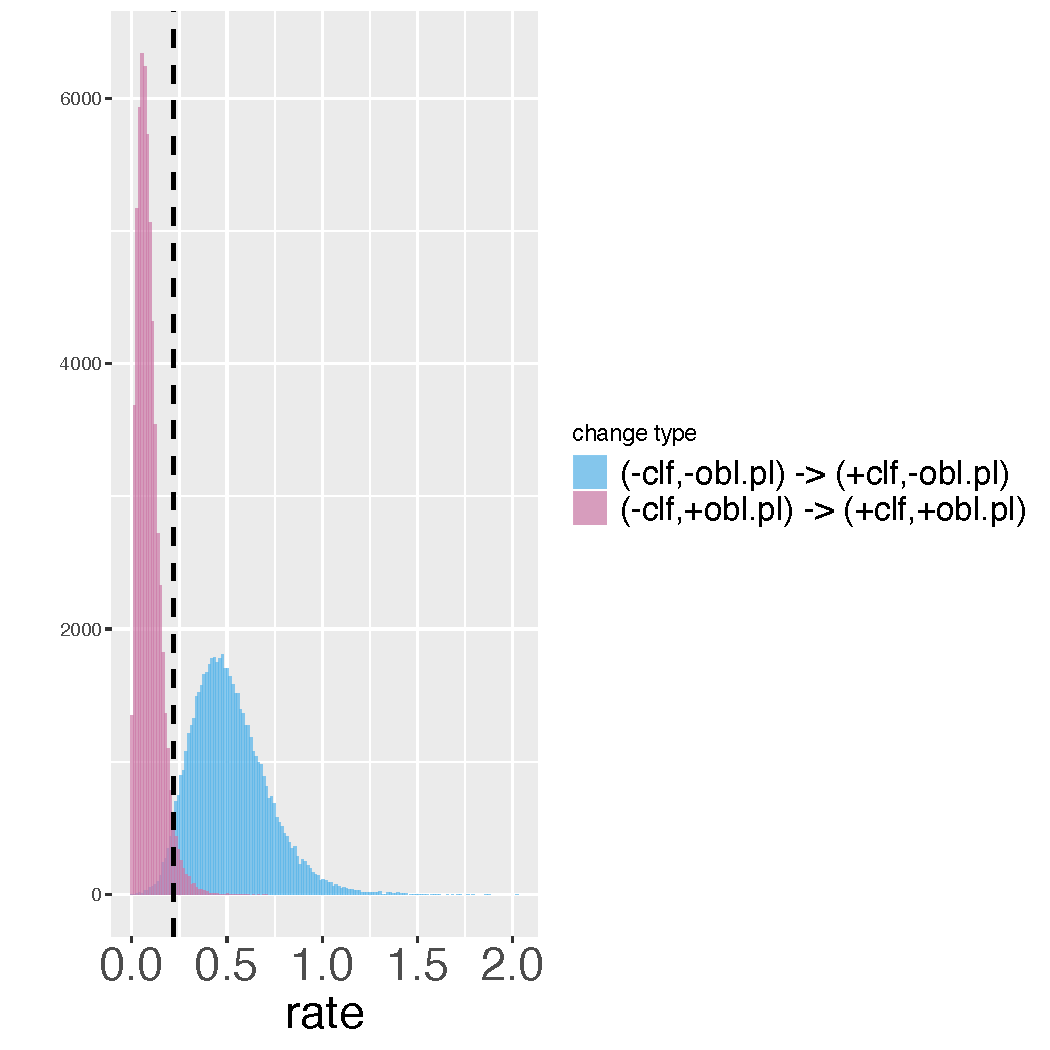
\includegraphics[width=\linewidth]{code/dia_rates.pdf}
\end{minipage}
\hspace{.05\linewidth}
\begin{minipage}[t]{.45\linewidth}
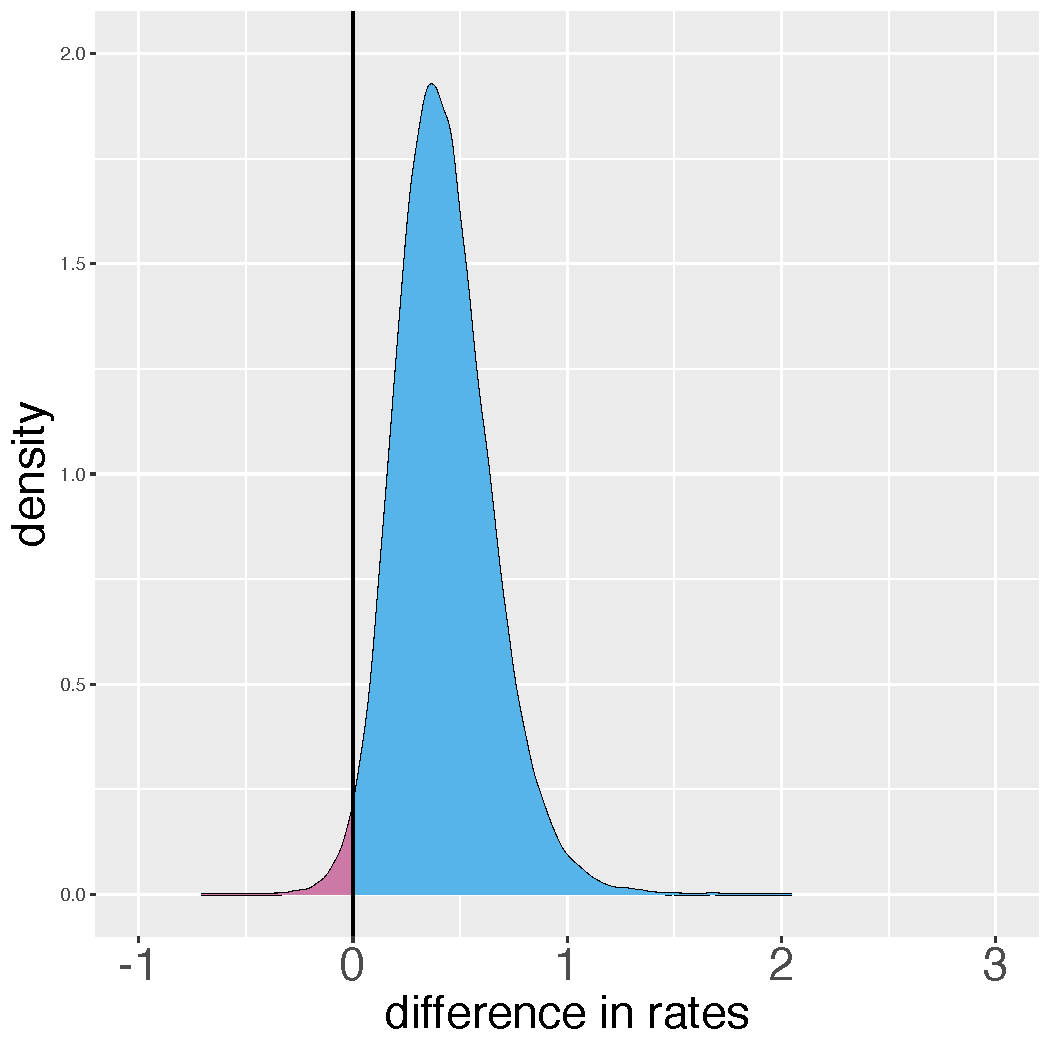
\includegraphics[width=\linewidth]{code/dia_diff.pdf}
\end{minipage}
\caption{Left: posterior distributions of rates for classifier gain given obligatory plural marking versus classifier gain given optional plural marking. Right: Difference between rates of classifier gain in the presence of optional versus obligatory plural marking; values greater than zero indicate that classifiers are gained more frequently in the presence of optional plural marking as opposed to obligatory plural marking.}
\label{dia_rates}
\end{figure}

The diachronic GSS hypothesis predicts that classifiers are gained more frequently in the presence of optional plural marking than in the presence of obligatory plural marking. We quantify this difference by comparing the posterior rates for the transition $q(\text{\sc ($-$clf, $-$obl.pl) $\rightarrow$ ($+$clf, $-$obl.pl)})$ with those for the transition $q(\text{\sc ($-$clf, $+$obl.pl) $\rightarrow$ ($+$clf, $+$obl.pl)})$. Figure \ref{dia_rates} gives these rates, as well as the difference between their posterior distributions (i.e., $q(\text{\sc ($-$clf, $+$obl.pl) $\rightarrow$ ($+$clf, $+$obl.pl)})$ subtracted from $q(\text{\sc ($-$clf, $-$obl.pl) $\rightarrow$ ($+$clf, $-$obl.pl)})$ for each sample in the posterior trace); positive values indicate a higher preference for classifier gain in the presence of optional plural marking. $98.4\%$ of posterior samples show a positive difference between the two rates, indicating substantial support for the GSS hypothesis in its diachronic form; the development of classifiers in Indo-Iranian languages appears to have been strongly influenced by the presence of optional plural marking, though this is not the case in 100\% of cases where classifiers developed. For this reason, we investigate branch-specific developments in detail by carrying out stochastic character mapping in \S\ref{SCM}, which allows us draw inferences regarding the most probable trajectory leading to the development of classifiers on each branch where they emerge in the tree. 

\subsection{Synchronic GSS Hypothesis}

\begin{figure}[h!]
%\begin{adjustbox}{max totalsize=\linewidth}
%\input{hypothesis_rates}
%\end{adjustbox}
\begin{minipage}[t]{.45\linewidth}
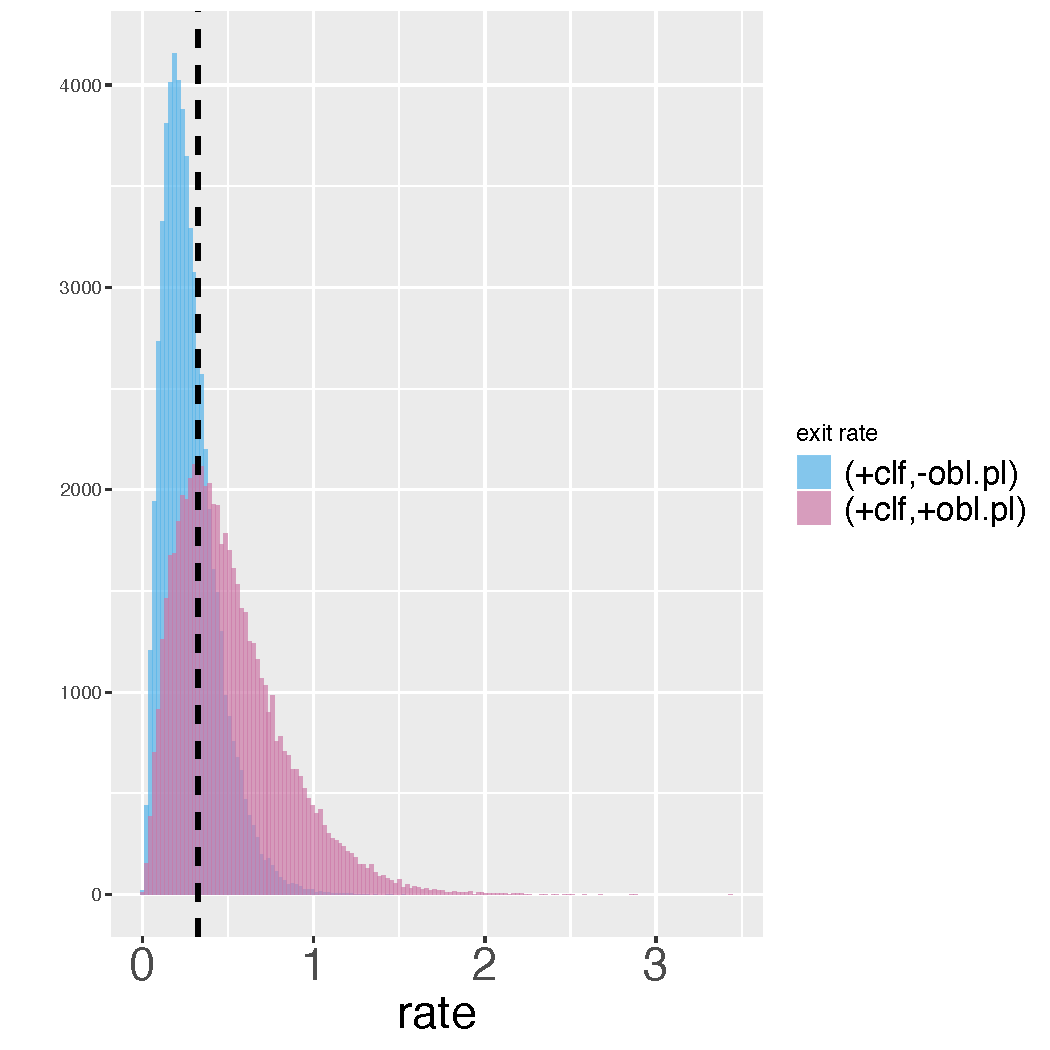
\includegraphics[width=\linewidth]{code/syn_rates.pdf}
\end{minipage}
\hspace{.05\linewidth}
\begin{minipage}[t]{.45\linewidth}
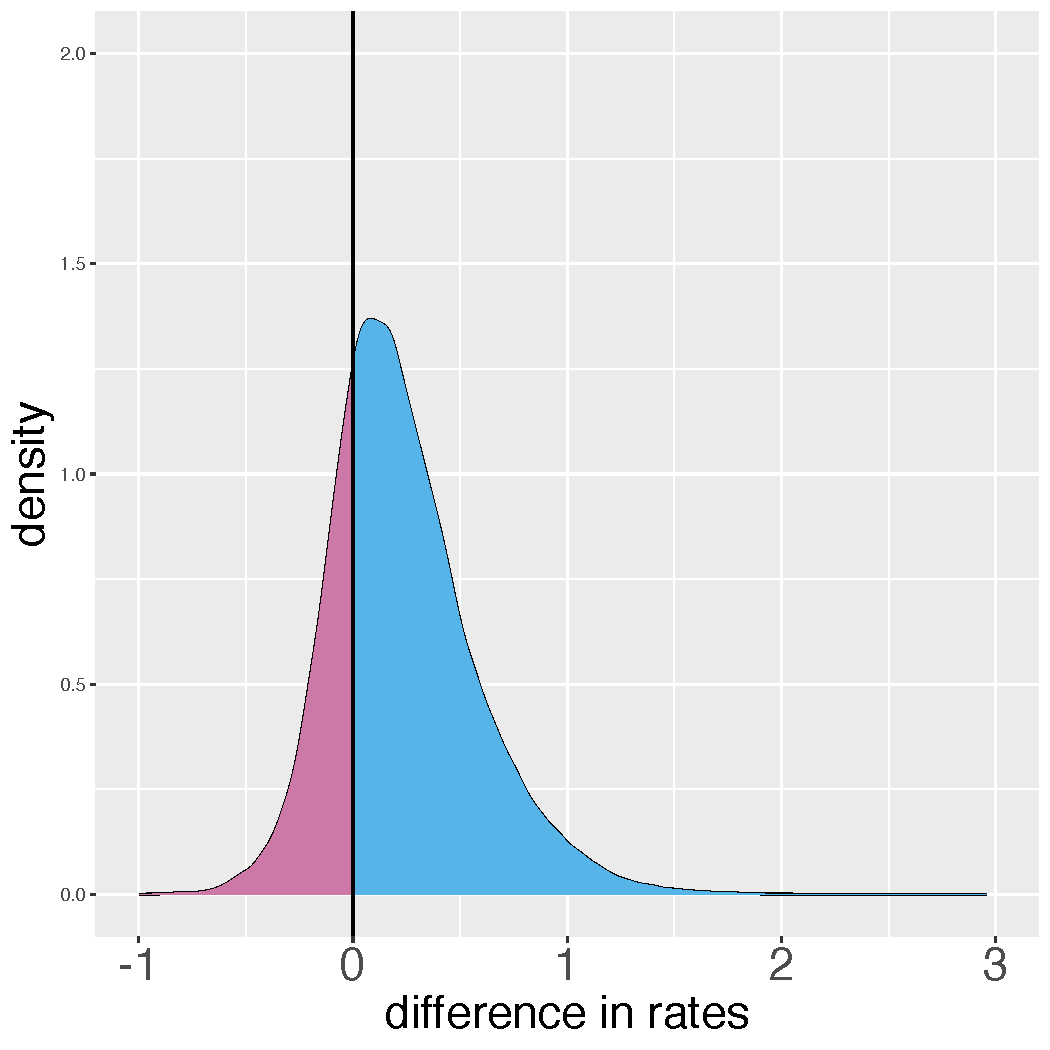
\includegraphics[width=\linewidth]{code/syn_diff.pdf}
\end{minipage}
\caption{Left: posterior distributions of exit rates for the states {\sc ($+$clf, $-$obl.pl)} and {\sc ($+$clf, $+$obl.pl)}. Right: Difference between exit rate for {\sc ($+$clf, $+$obl.pl)} and exit rate for {\sc ($+$clf, $-$obl.pl)}; values greater than zero indicate that {\sc ($+$clf, $+$obl.pl)} is abandoned at a higher rate.} 
\label{syn_rates}
\end{figure}

The synchronic GSS hypothesis predicts that the state {\sc ($+$clf, $+$obl.pl)} is synchronically dispreferred, and we expect this typological state to have a higher exit rate than the state {\sc ($+$clf, $-$obl.pl)}. 
The exit rate of a state can be computed by summing over all transition rates away from the state in question. Hence, the exit rates for the relevant states are the following:

\begin{align*}
q_{\text{exit}}(\text{{\sc ($+$clf, $+$obl.pl)}}) = & q(\text{\sc ($+$clf, $+$obl.pl) $\rightarrow$ ($+$clf, $-$obl.pl)})\\
& q(\text{\sc ($+$clf, $+$obl.pl) $\rightarrow$ ($+$clf, $-$obl.pl)})\\
& q(\text{\sc ($+$clf, $+$obl.pl) $\rightarrow$ ($-$clf, $-$obl.pl)})\\
\end{align*}
\begin{align*}
q_{\text{exit}}(\text{{\sc ($+$clf, $-$obl.pl)}}) = & q(\text{\sc ($+$clf, $-$obl.pl) $\rightarrow$ ($+$clf, $+$obl.pl)})\\
& q(\text{\sc ($+$clf, $-$obl.pl) $\rightarrow$ ($+$clf, $-$obl.pl)})\\
& q(\text{\sc ($+$clf, $-$obl.pl) $\rightarrow$ ($-$clf, $-$obl.pl)})\\
\end{align*}

We find, as shown in Figure \ref{syn_rates} that the exit rate for {\sc ($+$clf, $+$obl.pl)} is higher than the exit rate for {\sc ($+$clf, $-$obl.pl)}, but not substantially so; the difference in rates is greater than zero in only $75.6\%$ of samples. 
The fact that $24.4\%$ of samples are incompatible with the synchronic GSS hypothesis means that we cannot reject the null hypothesis that {\sc ($+$clf, $+$obl.pl)} and {\sc ($+$clf, $-$obl.pl)} are roughly equal in their stability. This shows that there is nothing inherently dispreferred about the cooccurrence of classifiers and obligatory plural marking; this state of affairs may arise less frequently through diachronic change than the state {\sc ($+$clf, $-$obl.pl)}: the more frequent trajectory {\sc ($-$clf, $-$obl.pl) $\rightarrow$ ($+$clf, $-$obl.pl)} may reflect a more general cognitive bias towards unitization, while the trajectory {\sc ($-$clf, $+$obl.pl) $\rightarrow$ ($+$clf, $+$obl.pl)} may occur for sociolinguistic and contact-based reasons.

\subsection{Character histories}
\label{SCM}

\begin{figure}[h!]
\centering
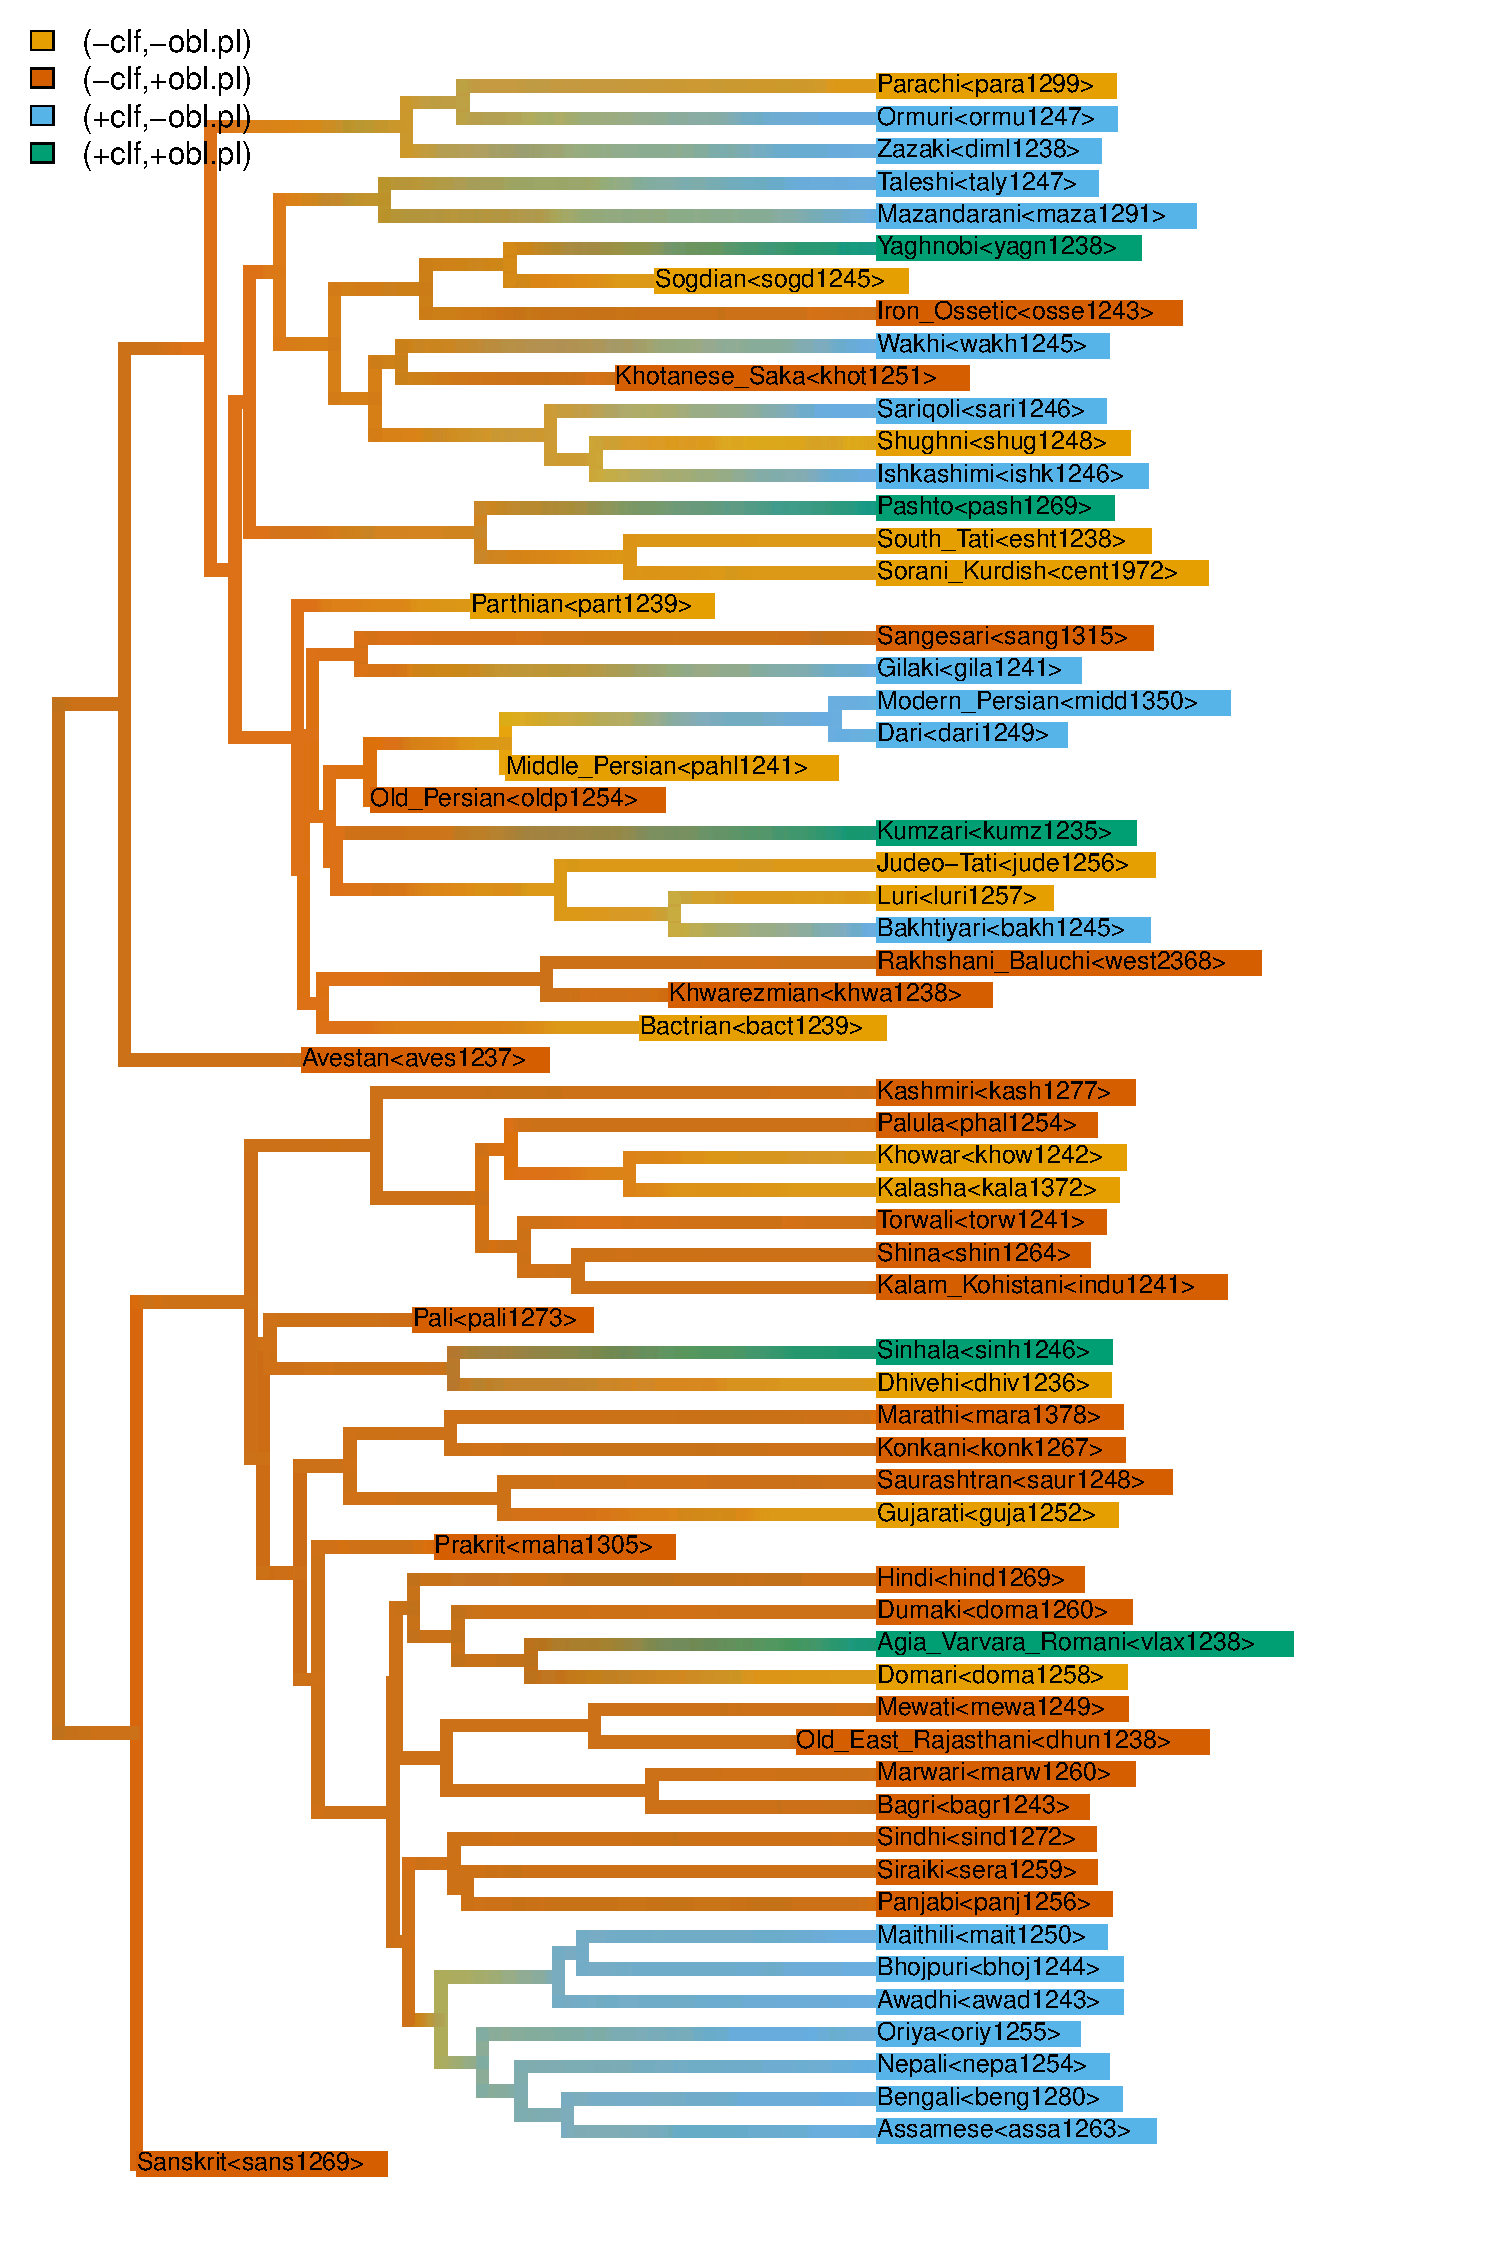
\includegraphics[width=.7\linewidth]{code/density_map.pdf}
\caption{Density map aggregating probable character histories over maximum clade credibility tree constructed from the tree sample.}
\label{densitymap}
\end{figure}


\begin{figure}[h!]
\centering
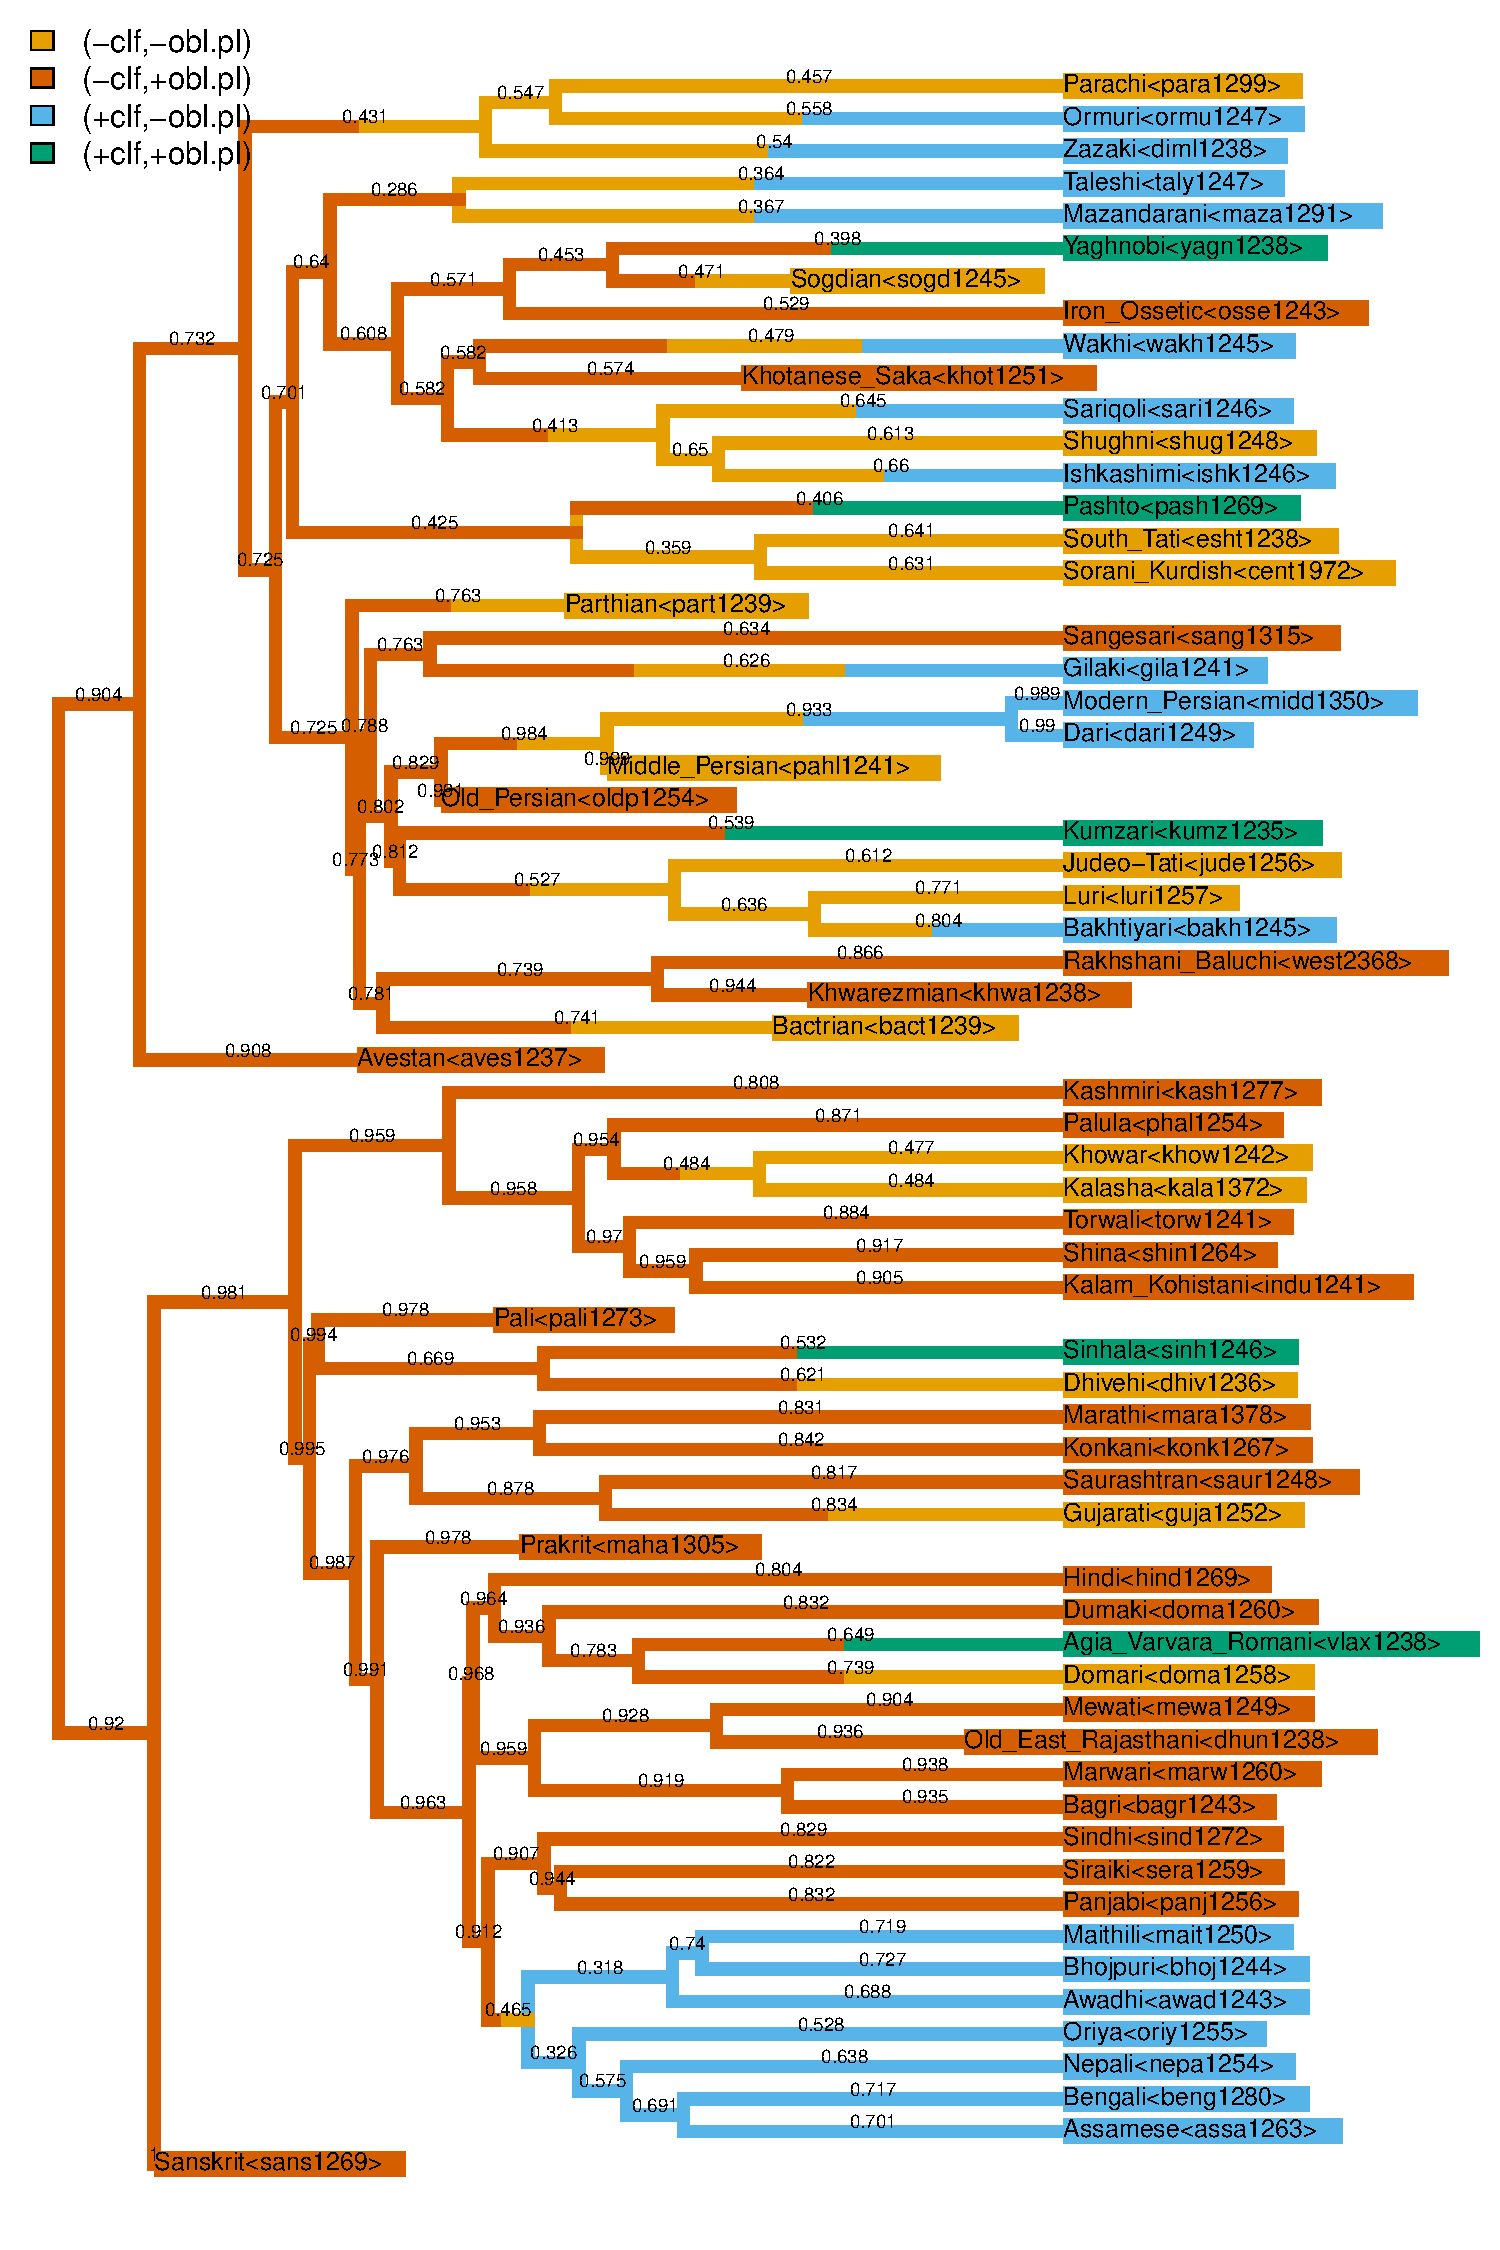
\includegraphics[width=.7\linewidth]{code/consensus_simmap.pdf}
\caption{MAP character history over maximum clade credibility tree constructed from the tree sample.}
\label{MAP}
\end{figure}

We carry out stochastic character mapping using the SIMMAP method \citep{Bollback2006} as implemented in the {\tt R} package {\tt Phytools} \citep{Revell2012}. We simulate character histories on the tree over 1000 iterations, drawing from the posterior sample of transition rates. 
The standard way for visualizing the aggregation of these histories is to use a density map, which represents the probability of a state in continuous space over the tree using a color gradient. Visualization can be a challenge for more than two states, since colors can become muddy in regions where uncertainty over the state value of the character is high. For this reason, we estimate a maximum a posteriori (MAP) character history over the tree by tabulating for each branch the counts for each type of transition history (ignoring the actual waiting times between transitions)
%{\color{red} irrespective of the times} at which each change occurs, 
and taking the most frequent transition history. 

We give both a density map and a MAP character history in Figures \ref{densitymap}--\ref{MAP}. Each branch is annotated according to the posterior support for its MAP transition history. 
%This procedure also allows us to estimate the probability of that a given state is present at each internal node of the tree, i.e., nodes in our tree where data are not observed. 
Striking differences in diachronic behavior between Indo-Aryan and Iranian can be observed. % in Figures \ref{densitymap}--\ref{MAP} 
In Indo-Aryan, classifiers emerge only three times (on branches ancestral to Sinhala, Agia Varvara Romani, and several Eastern Indo-Aryan languages), and their development is not preceded by a period of optional plural marking. 
In contrast, an overwhelming number of cases of classifier development in Iranian are preceded by periods of optional plural marking. 

To ensure that these patterns (and specifically, this difference across the two subgroups) is not simply an artifact of the topology of the maximum clade credibility tree, we carry out SCM on 1000 trees drawn from the tree sample, tabulating the number of times classifiers are gained in the presence of optional plural marking versus obligatory plural marking within Indo-Aryan and Iranian. 
The results of this procedure, shown in Figure \ref{ia_ir_scm}, indicate that for Iranian languages, classifiers develop more frequently in the presence of optional plural marking than in Indo-Aryan languages. 
Additionally, for each language with numeral classifiers, we note the most frequent state that preceded the development of classifiers in the lineage directly ancestral to the language. 
There are some discrepancies between the information presented in Figure \ref{MAP} and Table \ref{prev_state}; in many cases, the most frequent character history is outnumbered by non-identical character histories that all show the same state directly preceding the development of numeral classifiers --- for instance, the most frequent distinct character history on the branch leading to Sinhala is ($-${\sc clf}, $+${\sc obl.pl}) $\rightarrow$ ($+${\sc clf}, $+${\sc obl.pl}), but this trajectory is outnumbered by character histories that differ from each other but all show the state ($-${\sc clf}, $-${\sc obl.pl}) directly anterior to the state ($+${\sc clf}, $+${\sc obl.pl}) displayed by Sinhala. 
Furthermore, these relative frequencies do not always sum to one, since in a very small number of simulations, classifiers have been reconstructed at the root of the tree, and 
on certain lineages, states with classifiers are not preceded by states without classifiers. 
%on certain lineages, classifiers will be lost and regained, but on others, there is no {\tt previous state} lacking classifiers. 

\begin{figure}[t!]
%\begin{adjustbox}{max totalsize=\linewidth}
%\input{hypothesis_rates}
%\end{adjustbox}
\begin{minipage}[t]{.45\linewidth}
\includegraphics[width=\linewidth]{code/ia_transitions.pdf}
\end{minipage}
\hspace{.05\linewidth}
\begin{minipage}[t]{.45\linewidth}
\includegraphics[width=\linewidth]{code/iran_transitions.pdf}
\end{minipage}
\caption{Number of gains of numeral classifiers in the presence of optional versus obligatory plural marking for Indo-Aryan and Iranian over 1000 iterations of SCM.}
\label{ia_ir_scm}
\end{figure}


\begin{table}[h!]
\centering
\begin{tabular}{|l|ll|}
\hline
 & ($-$clf,$-$obl.pl) & ($-$clf,$+$obl.pl)\\
\hline
Assamese$*$ & 0.872 & 0.128\\
Bengali$*$ & 0.869 & 0.131\\
Oriya$*$ & 0.867 & 0.133\\
Awadhi$*$ & 0.869 & 0.131\\
Nepali$*$ & 0.872 & 0.128\\
Bhojpuri$*$ & 0.863 & 0.137\\
Maithili$*$ & 0.861 & 0.139\\
Agia Varvara Romani$\dagger$ & 0.189 & 0.811\\
Sinhala$*$ & 0.297 & 0.703\\
\hline
Ishkashimi$*$$\dagger$ & 0.952 & 0.048\\
Sariqoli$*$$\dagger$ & 0.945 & 0.055\\
Wakhi$\dagger$ & 0.905 & 0.095\\
Yaghnobi$\dagger$ & 0.524 & 0.476\\
Pashto$\dagger$ & 0.448 & 0.552\\
Mazandarani$*$$\dagger$ & 0.93 & 0.07\\
Taleshi$*$$\dagger$ & 0.946 & 0.054\\
Bakhtiyari$*$ & 0.899 & 0.101\\
Dari$*$$\dagger$ & 0.998 & 0.002\\
Modern Persian$*$$\dagger$ & 0.998 & 0.002\\
Kumzari$*$ & 0.355 & 0.645\\
Gilaki$*$$\dagger$ & 0.881 & 0.119\\
Zazaki$*$$\dagger$ & 0.936 & 0.064\\
Ormuri$*$$\dagger$ & 0.955 & 0.045\\
\hline
\end{tabular}
\caption{Relative frequencies of states directly preceding the development of classifiers in lineages of languages with classifiers, averaged over 1000 SCM iterations.}
\label{prev_state}
\end{table}

Ultimately our results show that the GSS has considerable explanatory power regarding the development of classifiers in Indo-Iranian, but it is clear that classifier development is not solely a response to optional plural marking. While most of the developments seen in Iranian are largely compatible with the GSS generalization, this is not the case for Indo-Aryan. 
In the following section, we analyze the developments shown above individually, assessing the role of different factors potentially underlying the development of numeral classifiers in Indo-Iranian speech varieties. 

\section{Discussion}
Overall, our results show that the GGS may account for a considerable number of incidences of classifier development in Indo-Iranian, but suggest that other factors such as contact may play a role as well, and furthermore that there may be some degree of interaction between these factors. 
When discussing areal effects, we draw a simple distinction between cases in which Indo-Iranian languages have participated in prestige-driven borrowing of classifiers, and cases where Indo-Iranian languages have taken on patterns of classifier use and/or number marking under circumstance of stable multilingualism. This framework suits the purposes of our paper's analysis, but draws upon larger theories of source/recipient agentivity \citep{Ross1996,Winford2005,MatrasSakel2007}. 
In this section, we integrate our model results with qualitative insights regarding Indo-Iranian contact history in order to sketch a plausible account of the development of classifiers across the subgroup. 

\paragraph{Indo-Aryan}
A striking aspect of the character history that we have inferred over the tree is that in Indo-Aryan languages, classifiers come about far less frequently than they do in Iranian. It is likely that a single development accounts for the presence of classifiers across Eastern Indo-Aryan. 
In each case of emergence, classifier development does not appear with high certainty to be preceded by a period of optional plural marking, counter to the GSS hypothesis.\footnote{The figures in Table \ref{prev_state} show that the state ($-${\sc clf}, $-${\sc obl.pl}) precedes the development of classifiers in these two languages in roughly 50\% of SCM iterations. This value is lower than what we expect, and may be an artifact of the exclusion of additional Romani varieties (where plural marking is obligatory) and data, however incomplete, from Old Sinhala (see below).} 
This state of affairs seems to favor language contact as a potential explanation; however, matter borrowing has taken place in only one Indo-Aryan language with classifiers: 
Agia Varvara Romani has clearly borrowed {\it tane} from Turkish (see above), likely due to the prestige of the latter language; this element is found in other Romani dialects in contact with Turkish \citep[204]{Matras2002}. 

%Sinhala
Unlike Agia Varvara Romani, the Sinhala classifier is inherited, and does not point explicitly to contact. 
Our model's results do not provide much information as to whether Sinhala developed classifiers in the presence of optional plural marking. 
Given the historical record, this seems unlikely; 
Modern Sinhala obligatory number marking is thought to have developed from an earlier stage where singular marking was non-obligatory \citep{NitzNordhoff2010}.\footnote{While it is not possible from the available historical record to date the development of the {\it denaa} classifier relative to the development of a more restrictive number marking system, it is possible that the former development took place while singular marking still exhibited a degree of optionality. Either way, neither a system with obligatory number marking nor a system with optional singular marking should give rise to numeral classifiers under the Greenberg-Sanches-Slobin hypothesis.} 
Incidentally, the Sinhala classifier construction is very similar to that of surrounding Dravidian languages, especially Tamil.  Sinhala {\it denaa} apparently still has its meaning `people' in other contexts \citep[passim]{Chandralal2010}. 
In Modern Literary Tamil \citep[112--114]{Lehmann1993}, numerals above one have a so-called pronominalized form with a suffix {\it -ar}. In Modern Spoken Tamil \citep[132--135]{Schiffmann1999}, pronominalized numerals higher than one add the noun {\it peeru} `name' instead, which can also mean `person'. In both languages the newly formed numeral can be used attributively or pronominally. If used attributively, it can precede or follow the head noun. In Literary Tamil, they have a marked genitive reading instead if preposed. In Spoken Tamil, they have a specific or definite reading if postposed. The similarities with Sinhala are striking. In all three languages there is [N [Num Clf]] word order as at least one possibility and there is a connection with animacy, non-animate or non-human entities being unmarked. Some Dravidian languages on the mainland have similar classifier-like constructions for humans. In Telugu, for instance, numerals above eight combine with the word {\it mandi} `persons', e.g. {\it padi-mandi} `ten persons' \citep[106--109]{KrishnamurtiGwynn1985}. %Because Sinhala {\it denaa} is cognate with classifiers in other Indo-Iranian languages, there is also the possibility that the construction is a retention in Sinhala that influenced the Dravidian languages of the area. 
%However, the direction of influence is not altogether clear. 
%More historical and diachronic research is necessary to clarify this point.

The diachrony of the development of numeral classifiers in Eastern Indo-Aryan languages like Bengali is poorly understood. There is some evidence that medieval East Indo-Aryan languages had optional plural marking. \citet[23]{Mukherji1963} states that Old Bengali lacks morphological number, but that ``plurality ... can be expressed by combining a singular noun with a number of words which denote plurality.'' It is not clear whether this feature co-existed with classifier use, as there is good reason to believe that this feature was suppressed in literary registers, our only source of data on languages of this sort \citep[cf.][]{BarzDiller1985}. 
If the historical scenario suggested by our results is accurate, a sweeping change of the type {\sc ($-$clf, $+$obl.pl)} $\rightarrow$ {\sc ($+$clf, $-$obl.pl)} took place in the history of Eastern Indo-Aryan. This development suggests a change in the general typological profile of these languages, possibly brought about by widespread language shift. 

Eastern Indo-Aryan languages with numeral classifiers are spoken in the vicinity of Dravidian (e.g., Kurux), Austroasiatic (especially Munda, e.g. Kharia), and Sino-Tibetan (especially Tibeto-Burman, e.g., Jero) languages, many of which also exhibit numeral classifiers. 
%The most likely explanation is an areal connection between these languages. Although it is often difficult to identify the exact pattern of diffusion, there are many clear cases of borrowing. Consider the following data.
%\begin{example} Kharia (Austroasiatic)
%\gll tin jhan lebu=ki
%three {\sc clf} person={\sc pl}
%\glt `three people' \citep[195]{Peterson2011}
%\glend
%\end{example}
%\begin{example} Kurux (Dravidian)
%\gll du{\IPA :}-{\IPA \:t}hu{\IPA :} xadd-ar
%two-{\sc clf} children-{\sc pl.hum}
%\glt `two children' \citep[114]{KobayashiTirkey2017}
%\glend
%\end{example}
%\begin{example} Jero (Sino-Tibetan)
%\gll dui g{\IPA O\:t} mi
%two {\sc clf} fire
%\glt `two fires' \citep[118, shortened]{Opgenort2005}
%\glend
%\end{example}
%Similar to the situation in Iranian, it is paradoxically often the Indo-Aryan numeral classifier system that is adopted by surrounding languages instead of the other way around. Kharia {\it jhan} derives from Sadri \citep[195]{Peterson2011}, Kurux {\it {\IPA \:t}hu{\IPA :}} from Bihari \citep[305]{KobayashiTirkey2017}, and Jero {\it g{\IPA O\:t}} from Nepali \citep[117]{Opgenort2005}. In both cases, Iranian and Indo-Aryan, one possible explanation for the unexpected pattern could be a substrate influence that might have led to the emergence of numeral classifiers based on autochthonous Indo-Iranian material (pattern borrowing). 
%Subsequently, because of the larger number of speakers and the higher prestige of Indo-Iranian languages, some of these numeral classifiers have been adopted by surrounding languages, often in combination with the Indo-Iranian numeral system (matter borrowing). Because of this, in several languages the autochthonous numerals and classifiers are restricted in use or have been entirely lost. For example, the Sino-Tibetan language Yakkha has borrowed the Nepali numeral system and only retains the autochthonous numerals from one to three, although the Nepali numeral for one is also employed. Today, the human numeral classifier {\it -pa{\ng}} can only be combined with the Yakkha numerals two and three \citep[105--106]{Schackow2015}. 
%Exactly the same pattern is observed in Belhare (as cited above). 
%
%Due to the large number of numeral classifiers and its eastern location, {Assamese} represents a special case among the Eastern Indo-Aryan languages. \citet[48--51]{Moral1997} has given conclusive evidence for the scenario that the Assamese numeral classifier system has been heavily influenced especially by Tibeto-Burman languages. Contact languages of Assamese include Sino-Tibetan (e.g., Bodo, Garo, Meche), Kradai (e.g., Khamti), and Dravidian languages (e.g., Malto). The Meche language, for example, exhibits a large amount of numeral classifiers, only some of which have been adopted from Nepali \citep[17--19]{Kiryu2008}. Among Dravidian languages, the largest inventory of numeral classifiers can be found in Malto that is also spoken in the vicinity of Assamese \citep[128--132]{Mahapatra1979}. 
%A large number of numeral classifiers are also present in the Kradai language Khamti.
Striking parallels with the behavior of East Indo-Aryan classifiers can be found in the Kradai language Khamti. 
In Khamti, [N Clf Num] word order has an indefinite reading with the numeral `one', while [N Num Clf] word order is definite. 
Interestingly, Assamese, Bengali, and Oriya have a connection of word order with definiteness, where [N Num Clf] word order is definite while [Num Clf N] order is indefinite. 
% BB: I think to make this relevant, we need to cite an IA example with the same word order effect.
%CC: added
\begin{example} Khamti (Kradai)
\gll kuun\textsuperscript{4}maau koo\textsuperscript{1} leeung\textsuperscript{3}
bachelor {\sc clf} one
\glt `a bachelor' \citep[8, shortened]{Inglis2007}
\glend
\end{example}
\begin{example}
\gll kuun\textsuperscript{4} saam koo\textsuperscript{1}
person three {\sc clf}
\glt `three people' \citep[11, shortened]{Inglis2007}
\glend
\end{example}
\begin{example} Bengali
\gll ch{\IPA O} -\d{t}a boi
six {\sc -clf} book
\glt `six books' \citep[136]{David2015}
\glend
\end{example}
\begin{example}
\gll boi ch{\IPA O} -\d{t}a
book six {\sc -clf}
\glt `the six books' \citep[137]{David2015}
\glend
\end{example}
While further parallels and matches in morphosyntactic pattern are needed in order to make a conclusive case for a shift from a language specifically like Khamti to Eastern Indo-Aryan, the striking differences from other Indo-Aryan languages, as well as the dynamics of change shown in the evolutionary scenario that we infer, lend support to the idea that the typological profile of Eastern Indo-Aryan languages is due to contact rather than diachronic trends realized elsewhere in Indo-Iranian.


\paragraph{Iranian}
In contrast to the situation in Indo-Aryan, 
Iranian languages on the other hand appear to have developed classifiers more frequently; classifiers emerge on nine independent branches within Iranian. 
The majority of these developments are preceded by stages with optional plural marking; ultimately, the state of affairs characterized by the GSS generalization appears to have been more active in Iranian than in Indo-Aryan, although if cognitive pressure is largely responsible for the development of classifiers in Iranian, it most likely interacted with areal pressure (both in the form of prestige borrowing and multilingualism), leading to the spread of this feature across languages. 

%\subparagraph{Persian}
The historical record makes it relatively clear that the development of full-fledged numeral classifiers in Persian was preceded by a prolonged period of optional plural marking, a state of affairs recapitulated by our SCM procedure. Our evolutionary model suggests that this was the case on branches leading to Wakhi; the Pamir languages Sariqoli, Shughni and Ishkashimi; Taleshi; and Kumzari as well. Hence, these developments are compatible with the claims made by the GSS hypothesis. However, contact may have also played a role; the proximity of Iranian languages to Turkic languages possessing classifiers cannot be ignored. 
As mentioned previously, Turkic and Iranian languages came increasingly into contact in post-Sasanian times. 
However, numeral classifiers are a likely to be a relatively late development, post-dating the onset of the Turkic expansion from about the 5th century CE \citep{Yunusbayev2015}. The Old Turkic (ca. 7th to 11th century) corpus contains no sortal numeral classifiers \citep[226]{Erdal2004}; however, the later literary language Chagatay (ca. 14th to 19th century) in Central Asia already exhibited certain classifiers, such as {\it ba\v{s}} `head' \citep[155]{Bodrogligeti2001}, and classifier use in modern Turkic languages is widespread, found among different branches of Turkic, including Kipchak (e.g., Tatar, \citealt[70]{ChenZongzhenYiLiqian1986}), Oghuz (e.g., Turkmen, \citealt[169]{Clark1998}), and Karluk (e.g., Uzbek, \citealt{Beckwith1998}). 
It is not clear whether this distribution reflects a widespread, relatively late diffusion of the feature under question throughout Turkic or the realization of some sort of drift or slant-like tendency on one hand, or the inheritance of a chronologically deep feature within the Turkic family. 
Complicating matters, Turkic classifiers are often Iranian loans; only in restricted occurrences do Iranian languages borrow Turkic classifiers (e.g., Sariqoli $\leftarrow$ Uyghur). 
Further research and more methodological development is needed to address the question of whether Turkic classifiers are due to Iranian influence, Iranian classifiers are due to Turkic influence, or both groups developed classifiers as a response to loosening restrictions on plural marking under the influence of widespread multilingualism. 

%\subparagraph{East Iranian}
In some cases, the presence of numeral classifiers in Iranian languages is clearly due to influence from other Iranian languages. 
The numeral classifiers found in Wakhi, Yaghnobi and certain Pamir languages are clearly identifiable as Tajik, given Tajik's importance as a lingua franca in the region where these languages are spoken. 
Pashto has likely borrowed the classifier {\it tana} (m.)/{\it teni} (f.) from a Turkic language, though it has been in the language long enough to be integrated into the gender system and participate in a phonological process. 

%\subparagraph{Kumzari}
In other cases, the role of contact is unclear. Kumzari, located in Oman and is separated from other Iranian languages by the Persian Gulf, exhibits the classifiers {\it -ta} and {\it -kas} (for human beings), formally identical to the Persian classifier {\it t\=a} and the Persian word {\it kas} `person'. Kumzari is genetically very close to Old, Middle, and modern Persian \citep{Skjaervo1989b}, though it is not clear that it is a descendant of Old or Middle Persian. Given the relative isolation of Kumzari, it is possible that it developed these classifiers in parallel with Persian due to drift, %(i.e., because an incipient tendency toward close nominal apposition )
but contact with another Iranian language is also a possibility, since there has been longstanding migration to Oman from the other side of the Persian Gulf \citep{Barth1983}.\footnote{Though the historical phonology of Kumzari is poorly understood, there is some evidence that it preserves the consonant of Old Iranian final {\it *-aka-}, given the ``etymologically latent {\it k}'' in the definite form {\it martk-\=o} \citep[38]{WalAnonby2015} $<$ {\it *marta-ka-}. Modern Persian does not preserve this consonant (cf. {\it t\=a} $<$ Middle Persian {\it t\=ag} `piece', most likely going back to an element {\it *t\=aka-}). However, Kumzari seems to show preservation only in contexts where the form is suffixed, making it impossible to determine whether the loss of {\it -k} in {\it -ta} is regular or reflects a Persian borrowing.} 
Under our phylogenetic model, there is approximately 60\% posterior probability that Kumzari developed the state ($+${\sc clf}, $+${\sc obl.pl}) after a stage of optional plural marking (see Table \ref{prev_state}); the development of obligatory plural marking may be due to contact with neighboring Arabic, which has obligatory plural marking. 

The remainder of Iranian languages with classifiers (e.g., Mazandarani, Taleshi, and Gilaki) share a core group of classifiers that are formally near-identical to Persian ones (e.g., {\it t\=a}), but as in the case of Kumzari, %it is challenging to invoke Persian contact 
%{\tt }
%there is no explicit evidence for Persian contact in the form of 
%sound change, 
it is difficult to determine whether these forms are inherited or borrowed on the basis of sound change; 
at the same time, the dominance of Persian  over these languages is well established \citep{Borjian2009}, lending circumstantial evidence to the notion that they are Persian loans. 
Some Northwest Iranian languages have classifiers not found in Persian, e.g., Taleshi {\it g{\textschwa}la} \citep{Paul2011,Stilo2018}, perhaps cognate to Judeo-Tati {\it gile} `time, instance' \citep[310]{Authier2012}. 
Many of these languages appear to have undergone a long-term trend toward optional plural marking. It is likely that classifiers spread through contact, but did so because of their utility and the cognitive enhancement they brought about. 

%{\tt possible that they caught on because they were beneficial and due to prestige language}.

%Unless this represents a later diffusion of the feature under question throughout Turkic or the realization of some sort of drift or slant-like tendency, these facts suggest a relatively early emergence of classifiers in Turkic even before the literary Chagatay language. Some Turkic languages, such as Uzbek \citep{Beckwith1998} or Uyghur \citep{TuohutiLitifu2012}, exhibit several numeral classifiers. Paradoxically, many of the numeral classifiers in Turkic languages represent borrowings from Iranian languages. For example, the classifiers {\it d\^ana} in Uzbek \citep[131]{Beckwith1998} and {\it dan\"a} in Uyghur derive from Iranian and usually combine with inanimate objects (e.g., book, car, house, pen, TV, watermelon, \citealt[158f.]{TuohutiLitifu2012}). In the Turfan dialect of Uyghur, {\it dan\"a} also combines with animate and human nouns (e.g., cow, grandchild, soldier, \citealt[107, 173]{Yakup2005}).

From the evidence surveyed, a picture emerges where in the majority of cases, Indo-Iranian classifiers developed as both a response 
to the individual effects of contact and optional plural marking, and likely via an interaction between the two. Iranian languages often use borrowed matter as numeral classifiers, regardless of whether plural marking is optional or obligatory, as shown in Table \ref{counts}. In some cases actual classifiers are borrowed (e.g., Zazaki {\it teney} from Turkish); in others, borrowed matter seems to have been repurposed as classifiers (e.g., Persian uses Arabic loanwords as classifiers in addition to inherited material, though they probably did not enter the language as such). 
However, Iranian languages with obligatory plural marking seem not to have developed classifiers from inherited matter. 
Yaghnobi has borrowed classifiers from Tajik. 
The case of Kumzari is ambiguous, as it is not clear whether its classifiers are Persian cognates or loans, or whether plural marking was obligatory in Kumzari when classifiers developed. 
With the exception of Romani dialects, Indo-Aryan languages appear to have taken on patterns of number marking and classifier use from neighboring languages of other stocks (e.g., Kradai and Dravidian). 
 
 
\begin{table}
{\small 
 \begin{tabular}{|p{.15\linewidth}||p{.25\linewidth}|p{.25\linewidth}|p{.25\linewidth}|}
 \hline
% \hline
  & Borrowed matter & Inherited & Both \\
 \hline
% \hline
 +clf,-obl.pl & Wakhi & Bhojpuri, Awadhi, Maithili, Nepali, Oriya, Bengali, Assamese, Bakhtiyari & Sariqoli, Ishkashimi, Zazaki, Modern Persian, Dari, Gilaki, Taleshi, Mazandarani, Ormuri \\
\hline
+clf,+obl.pl & Agia Varvara Romani, Pashto, Yaghnobi & Sinhala, Kumzari & \\
\hline
 \end{tabular}
 }
 \caption{Table showing whether numeral classifiers are based on borrowed or inherited matter in languages with numeral classifier systems.}
 \label{counts}
 \end{table}

%I think we can make the following argument: in the majority of cases, classifiers developed as both a response to optional plural marking *and* contact, and this was realized both by means of pattern and matter borrowing. In the Indo-Aryan pattern borrowing case, prestige was likely not a factor. For Iranian languages with (+clf,-obl), prestige may have been a factor in some isolated cases. Prestige borrowing is almost certainly responsible for the presence of classifiers in Ajia Varvara Romani, Yaghnobi, and perhaps Pashto, which have (+clf,+obl), but not for Sinhala, and it is not clear what is going on in Kumzari. Hence, classifier borrowing overwhelmingly serves to bring about cognitive benefits, but in the majority of the few cases where it does not bring about cognitive benefits, it tends to be due to emblematic pressure from a prestige language.

{\color{green} Ultimately, languages with non-obligatory plural marking have classifiers based on either inherited or borrowed matter, but languages with obligatory plural marking tend to have classifiers based {solely} on borrowed matter (except for Sinhala and maybe Kumzari). If languages of the latter type borrowed classifiers during a stage when plural marking was not optional, it was possibly because the prestige of the source language trumped the fact that numeral classifiers would bring no understandable cognitive benefit to a language with obligatory plural marking. 
Languages where the development of classifiers brought about a cognitive benefit as well may have borrowed their classifiers from source languages with and without relative prestige, and this is reflected by the combination of matter (pointing to prestige) and pattern (pointing to stable multilingualism) borrowing that they display. 
Further research at a wider phylogenetic scale is needed to conclusively address some of these questions.
Use of phylogenetic models designed to account for heterotachy (evolutionary rates that vary between different regions of the tree) may help to better capture clade-specific diachronic preferences, though our results show a clear difference in the evolutionary behavior of Indo-Aryan and Iranian without such a model.}


\section{Conclusions}
\label{conc}
Our findings suggest that the emergence of classifiers is often tied to optional plural marking, partially explainable by a statistical universal principle in line with the Greenberg-Sanches-Slobin generalization. 
At the same time, we find that classifiers emerged specifically under contact, reflecting local history and the contingencies of migration and trade. These results seem contradictory when one approaches the distribution of linguistic structures from the popular view that conceptualizes universal pressure and areal histories as conflicting, confounding, and competing factors. The contradiction is resolved, however, if we adopt the view from Distributional Typology \citep{Bickel2015Distributional} where emphasis is placed on the \emph{interaction} between universal and areal factors \citep{Bickel2014Areas}. 

From this perspective, the borrowing of classifiers (as matter or pattern) is not the mere product of historical contingency. Instead, this borrowing is driven by the decay in number marking, i.e. it follows the Greenberg-Sanches-Slobin generalization. Such a scenario explains our finding that classifiers were considerably more likely to be borrowed in the absence than in the presence of number marking. Areal effects alone cannot explain this difference, while universal effects alone cannot explain why classifiers entered through borrowing rather through spontaneous developments (e.g.\ by reanalyzing nominal juxtapositions, as in Hackstein's \citeyear{Hackstein2010} theory).

While our study supports a scenario of an interaction between universal and areal effects, we caution that our simplified coding scheme may not have picked up all relevant factors and that further research is needed to consolidate our conclusions. What is arguably the most urgent extension is a more fine-grained coding that captures the distribution of number marking over specific noun types, controlling for potential effects of a referential scale.



}



\bibliographystyle{chicagoa}
\bibliography{pre_pilot_bibliography}

\paragraph{Agia Varvara Romani [vlax1238] (+clf,obl.pl)}
Singular forms are always morphologically distinct from their plural counterparts, usually via the addition of a plural suffix or alternation of the final vowel \citep[23ff.]{Igla1996}. When a numeral greater than one modifies a noun, the noun is morphologically plural (p.\ 45). When the counted item consists of indefinite objects, then {\it -tane} ($<$ Turkish {\it tane} `piece, part') appears next to the numeral; anaphoric use of this classifier is obligatory (p.\ 45). 
\paragraph{Assamese [assa1263] (+clf,opt.pl)}
Assamese has a large inventory of sortal classifiers. Plural marking is optional \citep{Borah2012,Chowdhary2012}.
\paragraph{Avestan [aves1237] (-clf,obl.pl)}
Plural number is consistently marked, given rich agreement morphology \citep{HoffmannForssman2002}.
\paragraph{Awadhi [awad1243] (+clf,opt.pl)}
Classifiers are present; information regarding plural marking is difficult to extract from \citealt[115ff.]{Saksena1971}, but it appears to be optional.
\paragraph{Bactrian [bact1239] (-clf,opt.pl)}
In late Bactrian, case and number distinctions have been neutralized due to the loss of distinctions between final vowels, resulting in ``an unmarked form without ending ... which may be used with either sg. or pl. reference, and a marked pl. form'' \citep[40]{SimsWilliams2007}.
\paragraph{Bagri [bagr1243] (-clf,morph.pl)}
There are at least three declensional classes, in one of which the plural and singular direct forms are identical. The distinction between animacy and inanimacy, rather than ending in {\it -i} versus other segments, is made by the author, who explicitly states that the suffix {\it -\~{a}} is optional on animate nouns. This is almost akin to a mixture of a system like that of Hindi, where plural cannot be marked on some noun case forms, and a system where plural marking is truly optional.
\paragraph{Bakhtiyari [bakh1245] (+clf,opt.pl)}
Classifiers are present, and plural marking is variable \citep{AnonbyAsadi2014}.
\paragraph{Bengali [beng1280] (+clf,opt.pl)}
Bengali has a large repertoire of numeral classifiers \citep[135]{David2015}. Classifiers are obligatory with non-numeric quantifiers and lower numbers; optional with numbers ending in `hundred', `thousand', `lakh', etc. (p. 142). Numeral classifiers cannot cooccur with nouns denoting a countable unit, e.g., units of weight, currency, time, except in certain emphatic contexts (p. 142). Plural marking is non-obligatory (p. 76).
\paragraph{Bhojpuri [bhoj1244] (+clf,opt.pl)}
Numeral classifiers are present, and plural marking is non-obligatory \citep[120, 228, 230]{Tiwari1960}
\paragraph{Dari [dari1249] (+clf,opt.pl)}
Classifier use is common, but not obligatory; plural marking is optional; it is not clear if plural marking can co-occur with classifier use as in Standard Modern Persian (\citealt[74-5]{Kiseleva1985}; \citealt[58-9]{Ioannesjan1999}).
\paragraph{Dhivehi [dhiv1236] (-clf,opt.pl)}
For nonhuman nouns, plural marking is optional when plurality is clear from context \citep[59]{Gnanadesikan2017}.
\paragraph{Domari [doma1258] (-clf,opt.pl)}
Plural marking on enumerated nouns interacts significantly with whether the numbers are inherited Indo-Aryan forms or borrowed from Arabic (see \citealt[97, 188ff.]{Matras2012}). Plural number is optionally marked on nouns modified by 2--3 (inherited numbers), obligatory on nouns modified by 4--10 (Arabic numbers), and optionally marked on nouns from 11 upward (Arabic numbers).
\paragraph{Dumaki [doma1260] (-clf,obl.pl)}
For virtually all nouns, the singular form is distinguishable from the plural form \citep[24ff.]{Lorimer1939}; this is achieved via suffixation or a stem alternation.
\paragraph{Gilaki [gila1241] (+clf,opt.pl)}
\citet{Rastorguevaetal2012} list several classifiers. Classifier use is optional when enumerating nouns, but appears to be quite common and obligatory in anaphoric use. In all examples given of counted nouns, there is no overt plural marking on the head noun (regardless of whether a classifier is present). Plural can otherwise be marked by means of certain suffixes.
\paragraph{Gujarati [guja1252] (-clf,opt.pl)}
\citet[66--7]{Cardona1965} refers to the plural marker {\it -o} as ``optional,'' and it seems to largely be omitted when nouns are modified by a number greater than 1; so-called ``variable'' nouns display a special ``dependent stem form'' when they are semantically plural, regardless of the presence of the suffix {\it -o}.
\paragraph{Hindi [hind1269] (-clf,morph.pl)}
Hindi shows four declensional classes; the details of number marking are different for each one. Certain noun types are paradigmatically non-exhaustive; plural marking not morphologically possible on C-final masculine nouns in direct case \citep{Oberlies2005}.
\paragraph{Iron Ossetic [osse1243] (-clf,obl.pl)}
Plural number is marked on nouns by means of the suffix {\it -t-} \citep[117]{Thordarson2009}. In most contexts (except for contexts of enumeration, see below), use of {\it -t-} appears to be obligatory. When a noun is enumerated by a numeral greater than one, the noun is marked by the suffix -i (Digor), identical to the genitive suffix. According to \citet[132]{Thordarson2009}, this suffix continues the Old Iranian plural suffix {\it *-ah}. Nouns enumerated by numbers greater than one are always marked in a way that renders them distinct from singular nouns.
\paragraph{Ishkashimi [ishk1246] (+clf,opt.pl)}
Ishkashimi contains at least three classifiers; nouns modified by a numeral greater than 1 can appear in singular or plural form \citep[50]{Paxalina1959}.
\paragraph{Judeo-Tati [jude1256] (-clf,opt.pl)}
Plural is marked on nouns with the suffix {\it -ho} \citep[79]{Authier2012}. Overt plural marking on enumerated nouns seems virtually non-existent.
\paragraph{Kalam Kohistani [indu1241] (-clf,obl.pl)}
Kalam Kohistani achieves plural marking on a number of nouns via a vowel fronting process, which also is found in oblique forms of nouns, and appears to mark plural consistently on nouns \citep[21]{BaartSagar2004}. The word {\it khur} `foot' may show variability in plural marking, but it is not clear from the data given.
\paragraph{Kalasha [kala1372] (-clf,opt.pl)}
Plural marking is optional \citep[35--6]{Petersen2015}.
\paragraph{Kashmiri [kash1277] (-clf,morph.pl)}
According to \citet[190ff.]{WaliKoul1996}: ``plurals are formed from singular stems by vowel change, palatalization and suffixation. A few nouns stay invariant. Masculine plurals are formed differently than the feminine plurals.'' Mass nouns, most body parts, and borrowed English nouns use the same forms in both the singular and the plural. Masculine nouns do not change for plurality if they have certain phonotactic properties or are borrowed from Hindi/Urdu and English with a final consonant.
\paragraph{Khotanese Saka [khot1251] (-clf,obl.pl)}
Plural number is consistently marked, given rich agreement morphology \citep{Emmerick1989}.
\paragraph{Khowar [khow1242] (-clf,opt.pl)}
Plural marking appears to be optional on the basis of examples provided in \citealt{EndresenKristiansen1981}.
\paragraph{Khwarezmian [khwa1238] (-clf,obl.pl)}
Plural is consistently marked \citep{DurkinMeisterernst2009}.
\paragraph{Konkani [konk1267] (-clf,morph.pl)}
Certain noun categories have identical singular and plural endings in the direct case; otherwise, plural is consistently marked \citep[126ff.]{Almeida1989}
\paragraph{Kumzari [kumz1235] (+clf,obl.pl)}
From \citeapos{Thomas1930} description, plural marking appears to be obligatory. Kumzari numerals are nearly identical to their Modern Persian cognates; however, from seven upwards, the Kumzari numerals all end in {\it -t\=a}, which is analyzed as a suffix. For human beings, a suffix {\it -kay} attaches to the number one {\it yek(kay)}; for two onward, the suffix {\it -kas} is used. According to a newer description, the numeral classifier {\it -t\=a} or {\it -ta} in Kumzari can also occur on numerals below seven \citep[47]{WalAnonby2015}
\paragraph{Luri [luri1257] (-clf,opt.pl)}
According to \citet{MacKinnon2003}, plural marking is the same as in Modern Persian. No information regarding numeral classifiers is provided.
\paragraph{Maithili [mait1250] (+clf,opt.pl)}
Maithili has at least two classifiers \citep[v.\ 1, 117]{Burghart1992}. The suffix {\it -sab(h)} is an optional plural marker; when added to nouns that are inherently plural (e.g., vegetables), takes on the meaning ``X and such things.'' Some other suffixes exist for reference to persons, used in formal speech \citep[v.\ 1, 50-1]{Burghart1992}.
\paragraph{Marathi [mara1378] (-clf,morph.pl)}
Plural number must be marked on semantically plural nouns, except where morphologically impossible, e.g., masculine kinship terms, certain loanwords \citep[366--7]{Pandharipande1997}. \citet[11]{Emeneau1956} claims that Marathi has a classifier {\it ja\d{n}/ja\d{n}\d{\={\i}}} (f.) that appears``when nouns denoting persons are numerated by numerals higher than four (and optionally for two to four).'' \citet[243]{Lambert1943} says the following: ``When the numerals refer to persons, special forms are used instead of don, tin, car; to other numerals the word {\IPA z@\:n} (m. {\IPA z@\:n}, cf.fem. {\IPA z@\:na(n)}; f. {\IPA z@\:ni}, cr.fem. {\IPA z@\:ni(n)}) is usually added. This word is often added also to the special forms of {\it don}, {\it tin}, {\it car}.'' No examples are given. \citet[50]{Katenina1963} gives examples of the special forms {\it doghe}, {\it tighe}, {\it \'caughe}, as well as the forms {\it {\'\j}a\d{n}} (m.) and {\it {\'\j}a\d{n}\={\i}} (f.) `people' which show the latter form as a head noun, but never in close apposition with another (head) noun. The interaction between the numerals and {\it {\'\j}a\d{n}(\={\i})} is striking; however, other grammars gloss these special forms simply as `both', `the three', and `the four' respectively \citep[59]{DhongdeWali2009}. These forms appear in Old Marathi as substantivized numerals, e.g., {\it he tighe bh\=au} `these three were brothers' (\citealt{Tulpule1963}, apud \citealt[425]{Southworth1970}).
\paragraph{Marwari [marw1260] (-clf,morph.pl)}
There are at least three declensional classes, in one of which the plural and singular direct forms are identical. Plural number is marked on plural nouns, where morphologically possible \citep[20, 29]{Gusain2004}.
\paragraph{Mazandarani [maza1291] (+clf,opt.pl)}
Classifiers are present, and plural marking is optional \citep[9--10]{Nawata1984}.
\paragraph{Mewati [mewa1249] (-clf,morph.pl)}
There are at least three declensional classes, in one of which the plural and singular direct forms are identical. Plural number is marked on plural nouns, where morphologically possible \citep[20, 29]{Gusain2003}.
\paragraph{Middle Persian [pahl1241] (-clf,opt.pl)}
Middle Persian can mark plural with the suffixes {\it -h\=a} and {\it -\=an}, but plural is frequently unmarked on plural nouns \citep[223]{Skjaervo2009}.
\paragraph{Modern Persian [midd1350] (+clf,opt.pl)}
Modern Persian has several numeral classifiers, the most basic and widespread of which is {\it t\=a}, optionally used with numbers larger than one \citep[478]{WindfuhrPerry2009}. Plural marking is optional, but the noun being modified can be marked for plural number if it has specific reference \citep[195]{Mahootian1997}. Classifiers are obligatory in anaphoric use.
\paragraph{Nepali [nepa1254] (+clf,opt.pl)}
Nepali contains several numeral classifiers \citep[100]{Acharya1991}; plural number is marked with {\it -haru}; according to Acharya this marking is optional (pp.\ 98-9). From Acharya's examples, {\it -haru} can can co-occur with numeral classifiers (p.\ 100). According to Bhim Lal Gautam (p.c.), -haru is obligatory with human nouns; however, non-human nouns cannot co-occur with overt plural marking and a classifier.
\paragraph{Old East Rajasthani [dhun1238] (-clf,morph.pl)}
There are at least three declensional classes, in one of which the plural and singular direct forms are identical. Plural number is marked on plural nouns, where morphologically possible \citep{Metzger2003}.
\paragraph{Old Persian [oldp1254] (-clf,obl.pl)}
Plural number is consistently marked, given rich agreement morphology \citep{Kent1953}.
\paragraph{Oriya [oriy1255] (+clf,opt.pl)}
Oriya has several classifiers; plural marking is optional \citep{NeukomPatnaik2003}.
\paragraph{Ormuri [ormu1247] (+clf,opt.pl)}
According to \citet[133]{Kieffer2003}, classifiers are used as they are in Dari.
\paragraph{Pali [pali1273] (-clf,obl.pl)}
Pali generally maintains a clear morphological distinction between singular and plural; although the nominative singular and plural of ā-stems fell together due to regular sound change, a secondary plural suffix came into use in order to distinguish between the two numbers \citep[150--1]{Oberlies2001}
\paragraph{Palula [phal1254] (-clf,obl.pl)}
Plural is consistently marked on count nouns with one of five suffixes, which are accompanied in some cases by stem alternations \citep[103--4]{Liljegren2016}.
\paragraph{Panjabi [panj1256] (-clf,morph.pl)}
There are at least three declensional classes, in one of which the plural and singular direct forms are identical. Plural number is marked on plural nouns, where morphologically possible \citep[214--5]{Bhatia1993}.
\paragraph{Parachi [para1299] (-clf,opt.pl)}
Little information about interactions between numeral modification and number marking can be found in \citet{Kieffer2009}. According to \citet[50]{Morgenstierne1929}, plural marking is optional, and rare when a numeral modifies the noun. No information regarding classifiers is given.
\paragraph{Parthian [part1239] (-clf,opt.pl)}
\citet[272]{DurkinMeisterernst2014} describes a scenario for all of Middle West Iranian whereby plural marking is optional on all enumerated nouns, but animate nouns are more often marked for plural number than inanimates.
\paragraph{Pashto [pash1269] (+clf,obl.pl)}
Plural number appears to be consistently marked on Pashto nouns \citep[45ff.]{Penzl1955}; most paradigms are relatively complex and contain stem alternations. Numeral classifiers are possible, and co-occur with nouns marked for plural number, possibly with gender agreement (p.\ 82).
\paragraph{Prakrit [maha1305] (-clf,obl.pl)}
Plural number is consistently marked, given rich agreement morphology \citep{Woolner1928}.
\paragraph{Rakhshani Baluchi [west2368] (-clf,morph.pl)}
Nouns can be marked for indefiniteness and singularity via the suffix {\it -e}; otherwise, there is no morphological distinction between singular and plural \citep[3ff.]{Barker1969}.
\paragraph{Sangesari [sang1315] (-clf,morph.pl)}
Classifiers do not exist in Sangesari. According to \citet[70ff.]{AzamiWindfuhr1972}, plural is consistently marked on oblique nouns with the suffix {\it -uon}, but rarely on direct nouns, except for a restricted set of items.
\paragraph{Sanskrit [sans1269] (-clf,obl.pl)}
Plural number is consistently marked, given rich agreement morphology \citep{Macdonell1910}.
\paragraph{Sariqoli [sari1246] (+clf,opt.pl)}
Classifiers are present, and plural marking is optional \citep{Paxalina1971}.
\paragraph{Saurashtran [saur1248] (-clf,morph.pl)}
Plural number is marked on Saurashtran nouns by means of two suffixes, {\it -nu} and {\it -lu} (< Telugu) \citep[45--6]{Ucida1979}. When a numeral greater than one modifies a noun, the noun is plural, but certain non-human nouns (e.g., days, years) do not take plural form. 
\paragraph{Shina [shin1264] (-clf,morph.pl)}
Plural appears to be consistently marked on count nouns \citep{Schmidtetal2008}.
\paragraph{Shughni [shug1248] (-clf,opt.pl)}
Plural marking is optional, but classifiers do not appear to be present \citep{Zarubin1960}.
\paragraph{Sindhi [sind1272] (-clf,morph.pl)}
There are at multiple declensional classes, in one of which the plural and singular direct forms are identical. Irregular plurals can be found for kinship terms. Arabic words often have distinctive plurals borrowed from the source language. Plural number is marked on plural nouns, where morphologically possible \citep[27--8]{Egorova1966}.
\paragraph{Sinhala [sinh1246] (+clf,obl.pl)}
When animate nouns are modified by a numeral, the form of the numeral used is different from that which is used when an inanimate noun is modified by a numeral \citep[60]{Chandralal2010}. Plural marking is obligatory, when applicable.
\paragraph{Siraiki [sera1259] (-clf,morph.pl)}
Certain noun categories have identical singular and plural endings in the direct case; otherwise, plural is consistently marked \citep{Shackle1976}
\paragraph{Sogdian [sogd1245] (-clf,opt.pl)}
Some Sogdian heavy stem nouns show a form that is identical to the singular in plural contexts \citep[313]{Yoshida2009}.
\paragraph{Sorani Kurdish [cent1972] (-clf,opt.pl)}
According to \citet[45-6]{Blau1980}, the simple form of a noun can have either a singular or plural reading. In general, plural number is marked with the suffix {\it -an}.
\paragraph{South Tati [esht1238] (-clf,opt.pl)}
According to \citet[78]{Yarshater1969}, ``nouns modified by a numeral higher than one, or by an expression denoting plurality, are generally expressed in the plural in Chali [a particular dialect].'' Occasionally, however, the singular is used. In the other dialects, normally the singular is used for enumerated nouns. Plural marking otherwise seems to be the norm.
\paragraph{Taleshi [taly1247] (+clf,opt.pl)}
Taleshi has a number of numeral classifiers, use of which is non-obligatory \citep[181-2]{Paul2011}; additionally, ``any noun following a numeral phrase is generally in the singular.'' Elsewhere, plural number is marked with a suffix that varies from dialect to dialect.
\paragraph{Torwali [torw1241] (-clf,morph.pl)}
According to \citet[34]{Grierson1929}, if a noun ends in a vowel, it can take a plural-marking suffix -e; otherwise, the singular and plural forms are identical.
\paragraph{Wakhi [wakh1245] (+clf,opt.pl)}
Native Wakhi numeral forms are in competition with Tajik numeral forms \citep[89-90]{GruenbergSteblinKamenskij1988}. The word for twenty (bist) is borrowed from Tajik, but numerals 20-30 can combine bist with either Wakhi or Tajik forms in the digits place. A number of classifiers are borrowed from Tajik. Unlike the situation in Yaghnobi, these classifiers can be used with both Wakhi and borrowed Tajik numerals. Plural is marked with the suffix {\it -i\v{s}(t)} (p. 19), but this marking appears to be optional.
\paragraph{Yaghnobi [yagn1238] (+clf,obl.pl)}
According to \citet[21--2]{Xromov1972}, when numbers two and upward combine with nouns, the noun is found in the oblique singular form; if measure terms are used, the measure term is marked for oblique singular. The numerative {\it ta}, borrowed from Tajik, can be used, but only with Tajik numerals. Outside of the context of enumeration, {\it -t/d} is consistently used to mark plural number on nouns.
\paragraph{Zazaki [diml1238] (+clf,opt.pl)}
According to \citet[19ff.]{Paul1998}, a morphologically singular noun can be used in a generic sense, but nouns denoting a plurality, definite or indefinite, take the plural ending. Plural marking is non-obligatory. An apparent sortal classifier {\it teney} co-occurs with nouns marked both for singular and plural.

\end{document}
\documentclass[11pt]{article}
\usepackage{tipa}
\usepackage{fancyhdr}
\usepackage{hyperref}
\usepackage{amsmath}
\providecommand{\tightlist}{%
  \setlength{\itemsep}{0pt}\setlength{\parskip}{0pt}}
\usepackage{authblk}
\usepackage{booktabs}
\usepackage{fullpage}
%\usepackage{kpfonts}
\usepackage{covington}
%\usepackage{XCharter}
\usepackage[T1]{fontenc}
\newcommand{\tsup}[1]{\textsuperscript{#1}}
\usepackage{adjustbox}
\usepackage{microtype}
\usepackage{caption}
\usepackage{tikz}
%\usepackage{gb4e}
\usepackage{setspace}
\usepackage{authblk}
\def\citeapos#1{\citeauthor{#1}'s (\citeyear{#1})}
\usepackage{natbib}
\Roman{section}
\bibpunct[:]{(}{)}{,}{a}{}{,}
\usepackage[utf8]{inputenc}
\usepackage{color}
%\usepackage{fontspec} % This line only for XeLaTeX and LuaLaTeX
\usepackage{pgfplots}
%\title{Classifiers and number marking in Indo-Iranian: an evolutionary study}
\title{Cognitive pressure, areal contact, or both? An evolutionary study of classifiers and number marking in Indo-Iranian}
%\author{Chundra Cathcart \hfill Andreas H\"olzl\\
%Paul Widmer \hfill Balthasar Bickel\\
%University of Zurich}
\author[1,2]{Chundra Cathcart}
\author[1,2]{Andreas H\"olzl}
\author[2]{Gerhard J\"ager}
\author[1,2]{Paul Widmer}
\author[1,2]{Balthasar Bickel}
\affil[1]{Department of Comparative Language Sciences, University of Zurich}
\affil[2]{Center for the Interdisciplinary Study of Language Evolution, University of Zurich}
\affil[3]{Department of Linguistics, University of T\"ubingen}

\date{}


\begin{document}
\maketitle
\sloppy

\begin{abstract}
\noindent This paper investigates the origins of sortal numeral classifiers in the Indo-Iranian languages. 
Due to the fact that classifiers are absent from most Indo-European languages, it is often assumed that Indo-Iranian classifiers are due to contact with non-Indo-European languages. 
An alternative possibility is that classifiers developed in Indo-Iranian languages as a response to the rise of optional plural marking, in line with the so-called Greenberg-Sanches-Slobin (henceforth GSS) generalization, which holds that the presence of sortal numeral classifiers across languages is negatively correlated with obligatory plural marking on nouns. 
We seek to assess the extent to which Indo-Iranian classifier development is influenced by loosening of restrictions on plural marking using a Bayesian phylogenetic model, inferring posterior distributions over evolutionary transition rates between typological states, and subsequently using these rates to reconstruct the history of classifiers and number marking throughout the family, constrained by historically attested states. 
We find substantial but not totally unambiguous support for the GSS hypothesis; some instances of classifier development follow a prolonged period of optional plural marking, while others do not. 
Further inspection of the most likely diachronic trajectories in individual lineages in the tree, as well as a survey of the matter and pattern borrowing that has taken place in attested languages, suggests that classifiers have come about due to the individual effects of optional plural marking and language contact, and possibly due to interactions between these factors as well. 
Interestingly, the effects of the GSS appear more strongly among Iranian languages, while Indo-Aryan languages seem to have developed classifiers solely due to contact. 
Taken as a whole, these findings tentatively suggest that the association of classifiers and optional number marking in Indo-Iranian is neither solely the effect of universal mechanisms nor of the contingency of local contact histories. 
\end{abstract}

\section{Introduction}
Indo-Iranian languages display considerable diversity in constructions where items are enumerated. 
Attested ancient (and to some extent medieval) languages such as Sanskrit and Avestan, which possess richer nominal morphology,  show a straightforward pattern where numerals or quantifiers and enumerated nouns agree fully in gender and number; however, contemporary languages do not consistently mark plural number on semantically plural nouns. 
Additionally, a number of Indo-Iranian languages make use of sortal numeral classifiers, as in the Bengali example {\it ch{\IPA O}-\d{t}a boi} `six books', where {\it \d{t}a} is a classifying element that co-occurs with an enumerated entity. 

This behavior is typologically uncharacteristic of the larger Indo-European family and it has therefore been attributed by some researchers to contact with languages from other stocks \citep{Emeneau1956,Emeneau1965,Matisoff1978,ThomasonKaufman1988}.
Others see Indo-Iranian numeral classifiers as the grammaticalized outcome of a general tendency seen in ancient and medieval Indo-European languages where generic and non-generic nouns are placed together in close apposition, which can potentially lead to systems of nominal classification \citep{Hackstein2010}. An important confound in resolving this debate is the extent to which languages are subject to what is known as the Greenberg-Sanches-Slobin generalization \citep{Greenberg1972,SanchesSlobin1973}. This generalization posits an association between the presence of numeral classifiers in a language with optionality (or even absence) of plural marking. If numeral classifiers develop to a stronger extent in languages with optional than in languages with obligatory number marking, their emergence in Indo-Iranian might reflect a general tendency of the sort argued for in the Greenberg-Sanches-Slobin hypothesis. If not, Indo-Iranian classifiers may have arisen due to contingencies of the family's history, especially its contact history.

This paper explores the diachronic pathways by which the diverse patterns seen in Indo-Iranian have developed. 
We employ an explicit phylogenetic approach to this question, inferring evolutionary transition rates between typological states concerning the presence of numeral classifiers and optionality of plural marking. 
First, we use these rates to operationalize the Greenberg-Sanches-Slobin hypothesis by observing whether the rate of classifier development is higher in the presence of optional plural marking than in the presence of obligatory plural marking. 
Subsequently, we use these rates to infer the most likely diachronic trajectories in individual lineages in the tree, allowing us to identify different pressures in the development of classifier marking over the tree. 
We find that neither the Greenberg-Sanches-Slobin generalization nor language contact alone can account for all instances of classifier development in Indo-Iranian. 
Indo-Aryan languages appear to have developed classifiers due to stable multilingualism with languages from non-Indo-European stocks. 
Iranian languages, on the other hand, appear largely to have developed classifiers largely after prolonged periods of optional plural marking, in line with the GSS. Given what is known about the sociopolitical history of the Iranian-speaking area as well as the pattern and matter borrowing  \citep{MatrasSakel2007} that we observe in our data set, we tentatively conclude that Iranian classifiers are a response to optional plural marking that was helped along by widespread multilingualism. 

In what follows, we describe the Greenberg-Sanches-Slobin generalization in more detail (Section \ref{background}). We then provide a detailed description of the synchronic and diachronic patterns seen in Indo-Iranian constructions where items are enumerated (Section \ref{sec-ii}). After introducing our data coding and the inference model (Section \ref{methods}), we present and discuss our main findings (Sections \ref{res}--\ref{conc}).


\section{Background}
\label{background}

\subsection{Numeral Classifiers}
Numeral classifiers (alternatively called numeratives; cf.\ \citealt[98]{Aikhenvald2000}) are usually contiguous to numerals in expressions of quantity or, more generally, found to occur in the context of quantification \citep[63]{Grinevald2000}.
In this study, we define a numeral classifier as any morpheme that, independent of its morphosyntactic status, is linearly adjacent to a numeral (or an equivalent quantifier) when it occurs, %(e.g., numeral interrogative or demonstrative), 
% BB: what is a numeral interrogative? I have never seen this term. If you intend expressions like 'how many', 'that many', that would be quanitifiers and the bracketed explanation can go.
%CC: commented out offending text
functioning with the numeral as an attribute of a head noun. A numeral classifier tends to have mutual dependencies (e.g., collocational, morphosyntactic, phonological, or semantic) with the numeral and the head noun. In the following example of Mandarin Chinese, for instance, the noun {\it sh\=u} `book' can only be combined with the numeral classifier {\it b\v{e}n}. Furthermore, the numeral {\it li\v{a}ng} replaces the general numeral {\it \`er} `two' in numeral classifier constructions. If {\it b\v{e}n} is not preceded by a numeral it has a set of different meanings.
\begin{example} Mandarin (Sino-Tibetan)
\gll li\v{a}ng b\v{e}n sh\=u
two.{\sc clf} {\sc clf} book
\glt `two books'
\glend
\end{example}
Numeral classifiers usually form a constituent with the numeral rather than with the head noun \citep[e.g.,][105]{Aikhenvald2000}; the noun can never occur in between the numeral and the classifier \citep{Her2017}.

Numeral classifiers are generally divided into mensural and sortal subtypes. Mensural classifiers aid in partitioning an uncountable noun (e.g., Modern German {\it ein Glas Bier} `a glass of beer'), and are usually considered to be distinct from pseudo-partitives (e.g., Middle High German {\it ein glas bier-s} `a glass of beer', \citealt[33]{Bauer2017}) in that the noun is not marked in a way that differs across enumerated and non-enumerated contexts.
Sortal classifiers, by contrast, are not limited to uncountable nouns, and have been defined variously as:
\begin{itemize}
\item A member of a paradigm that forms a binary phrase with a numeral, which in turn forms a binary phrase with a counted noun \citep{Lehmann2000}
\item A grammatical element that occurs with nouns (regardless of their degree of countability) in construction with numerals \citep{Gil2005}
\item An expression that indicates a unit of counting or measure \citep{Doetjes2012}
\end{itemize}
Unlike mensural classifiers, sortal classifiers cannot be modified by an adjective: expressions like {\it ein kaltes Glas Bier} `a cold glass of beer' have no equivalent with sortal classifiers; sortal classifiers generally cannot co-occur with mensural classifiers, e.g., Maithili {\it das(*-\d{t}\=a) kap c\=ay} `ten (*{\sc clf}) cup tea' \citep[I:117]{Burghart1992}. 
A third type of numeral classifier designates groups, similar to English {\it a flock of birds} \citep[e.g.,][131--133]{Beckwith1998}. Such classifiers indicate a set larger than one, including a pair. Sortal and mensural numeral classifiers do not indicate any number on their own, but are differentiated by the type of noun they occur with. Most languages exhibit numeral classifiers that refer to measures and groups. This study exclusively focuses on sortal numeral classifiers, which are much less common cross-linguistically and exhibit a very specific geographic distribution.

While a numeral classifier can provide an index to inherent semantic properties of the head noun (its use is often dependent on these properties) and can also carry pragmatic meaning, it does not achieve semantic modification in the way that adnominal elements such as adjectives do.\footnote{In some languages, elements identical to numeral classifiers also occur in bare use with nouns, marking them variously for definiteness or indefiniteness \citep{Simpsonetal2011}. Though these are often referred to as ``bare numeral classifiers,'' they fall outside the scope of our definition.}
Furthermore, anaphoric use is common, in which case the head noun is excluded.
We are additionally agnostic to the status of classifiers as a full phonological word, since they at times fuse phonologically with the numeral.


\subsubsection{Indo-Iranian Classifiers}
The diachrony of Indo-Iranian numeral classifier systems is not well understood given lacunae in the historical record, making it difficult to determine whether they developed as a response to the loosening of restrictions on plural marking, because of contact, or due to other factors. 
Attestations of classifiers are largely absent from pre-modern Indo-Aryan languages, e.g., Old Bengali, perhaps due to stigmatization and suppression in the literary register (for discussion, see \citealt[168]{BarzDiller1985}). 
It is however possible to trace the development of certain numeral classifiers in the history of Persian, though the material is incomplete and the exact pathway of development is somewhat ambiguous. 
In the absence of evidence from this historical record, it is in theory possible to infer whether classifiers developed due to language contact on the basis of (1) the presence of matter borrowing and (2) languages' proximity to groups with numeral classifiers, but again, the picture is not entirely clear. 

On the whole, Indo-Iranian classifiers are a mix of inherited and borrowed material. 
Agia Varvara Romani has borrowed the classifier {\it -tane} from Turkish\footnote{The Turkish form is generally thought to be an Iranian loan cognate to Persian {\it d\=anah} `grain', with devoicing of initial {\it d-} \citep[138]{Stilo2018}.} (and has obligatory plural marking):
\begin{example}
\gll Dikhl\'em p\'and\v{z}tane rakl\'a
see.1{\sc sg.pst} 5.{\sc clf} girl.{\sc pl.acc}
\glt `I saw five girls' \citep[45]{Igla1996}
\glend
\end{example}
The classifiers found in Indo-Aryan languages of South Asia tend to belong to a core group of elements with transparent Old Indo-Aryan (OIA) etymologies, which are supplemented with additional classifiers (Assamese has roughly a dozen numeral classifiers, all of which appear to be from inherited Indo-Aryan material). 
%The remaining Indo-Aryan languages with classifiers generally possess a core group of elements with transparent Old Indo-Aryan (OIA) etymologies. 
The most geographically widespread Indo-Aryan classifier is a reflex of Old Indo-Aryan {\it jana-} `person', occurring in Sinhala as the element {\it denaa} \citep[4]{Geiger1942} as well as in Eastern Indo-Aryan languages. 
Another common classifier (Nepali {\it va\d{t}\=a}; Bengali, Oriya, {\it \d{t}\=a}; Assamese {\it t\=a}) is derived by \citet[684ff.]{Chatterji1926} from OIA {\it v\textsubring{r}t-ti-ka-}, a deverbal noun built to the root {\it vart-} `turn'.
The classifier {\it go\d{t}}, found in Maithili and other Eastern Indo-Aryan languages, continues Old Indo-Aryan {\it g\={o}\d{t}\d{t}a-} *`something round' \citep[229]{Turner1962}. 
With the exception of Sinhala, the aforementioned languages have optional plural marking on most noun types, and tend to prohibit plural marking on enumerated nouns that co-occur with numeral classifiers:
\begin{example} Maithili
\gll s\=at -\d{t}\=a murg\={\i} (*-sabh)
seven {\sc clf} hen {\sc pl}
\glt `seven hens' \citep[117]{Burghart1992}
\glend
\end{example}
However, in Nepali, referential scales may require plural marking in some circumstances, leading to the co-occurrence of numeral classifiers and plural marking:
\begin{example} Nepali
\gll c\=ar jan\=a mitra *(-haru)
4 {\sc clf} friend {\sc pl}
\glt `four friends' (Bhim Lal Gautam, p.c.)
\glend
\end{example}

Iranian languages employ a more varied mix of inherited forms and borrowed elements from Arabic as well as Turkic languages. 
Modern Persian employs a number of Arabic terms in addition to the inherited classifier {\it t\=a}. It seems unlikely that Persian borrowed these items as classifiers {\it per se}, since the syntactic patterns characterizing Persian classifier use differ from those of Arabic dialects with numeral classifiers.\footnote{For instance, Persian employs a numeral classifier {\it ra's} `head' ($<$ Arabic) for animals. \citet[18--20]{Greenberg1972} cites constructions from a 19th century Arabic dialect of Oman and Zanzibar %(an unlikely donor with respect to Persian to begin with) 
which employs the same word when counting animals, but in contrast to Persian usage, it inflects for number.} 
These classifiers of Arabic origin can be found in related Iranian languages. 
Classifiers of Turkic origin are found as well. Zazaki {\it teney} is a Turkish loan (the same element is found in Agia Varvara Romani), and Pashto {\it tana/teni} may be from a Turkic source as well, though these forms are ultimately Iranian back loans. The Sariqoli classifier {\it tol} may be of Turkic origin (cf.\ Uygur {\it tal}).

The full range of circumstances under which Iranian classifiers developed is unknown, but Middle and Early Modern Persian provide a window onto the usage of the precursor of the Modern Persian general classifier {\it t\=a}, which continues Middle Persian (Pahlavi) {\it t\=ag}, a multifunctional element glossed as `item, unit, alone, single' by \citet{Mackenzie1971}, who keeps this headword separate from {\it t\=ag} `branch'.
The following examples from the Pahlavi Wid\=ewd\=ad show a diverse range of uses:
\begin{examples}
\item \gll nay \=ew t\=ag
reed one piece
\glt `a single piece of reed' \citep[272]{Moazami2014}
\glend
\end{examples}

\begin{examples}
\item \gll \=ew t\=ag fr\=az \=o \=atax\v{s} dah\=ed
one piece forward to fire give.{\sc imper}
\glt `give once to the fire' \citep[254]{Moazami2014}
\glend
\end{examples}

\begin{examples}
\item \gll b\=ob -\=e b\=ali\v{s}n se t\=ag
fine\underline{\phantom{ }}carpet {\sc indef} pillow three piece
\glt `a fine carpet (and) three-fold cushions' \citep[352]{Moazami2014}
\glend
\end{examples}

\begin{examples}
\item \gll spi\v{s} -\=e ay\={a}b ri\v{s}k -\=e t\=ag
louse {\sc ez} or nit {\sc ez} piece
\glt `a single louse or nit' \citep[390]{Moazami2014}
\glend
\end{examples}


\begin{examples}
\item \gll u -\v{s} n\=o -\={\i}h t\=ag w\=ed bar\={\i}d
he {\sc 3sg} nine {\sc abstract.suffix} branch willow bring.{\sc pst.3sg}
\glt `he brought nine branches\footnote{\citet{Mackenzie1971} keeps the headwords for `branch' and `item' separate. Regardless of whether these entries should be separate, the use of `branch' as a mensural classifier here is noteworthy. We see also the reduplicative plural {\it t\=ag t\=ag} \citep[122]{Moazami2014}.} (of {\it barsom})' \citep[468]{Moazami2014}
\glend
\end{examples}
\citet[171]{Mache2012} cites the following example, in which {\it t\=a(g)} appears to be used as a sortal classifier:
\begin{examples}
\item \gll \v{c}and t\=a d\=an\=ag\=an \={\i} hind\=ug\=an
some t\=a wise.{\sc pl} {\sc ez} Indian.{\sc pl}
\glt `some wise Indian men'
\glend
\end{examples}
She argues on the basis of this example that Middle Persian is a classifier language, though the evidence is quite restricted. %It is worth noting that the head noun here most likely has non-specific reference, while
We refrain from treating Middle Persian as a numeral classifier language, given the scant, rather ambiguous evidence and the fact that the loose morphosyntactic integration of information in noun phrases containing {\it t\=ag} makes it difficult to determine whether they meet the criteria we have chosen for numeral classifiers. 

Numeral classifier constructions like those seen in Modern Persian are not attested in Early Modern Persian. However, some constructions involving {\it t\=a} `piece, unit' are found in Early Modern Persian. 
In these constructions, {\it t\=a} marked for indefiniteness is followed by a number or quantifier.\footnote{Lazard states that this construction --- e.g., indefinite nouns followed by a number or quantifier --- indicates an order of magnitude for large numbers (``nombres ronds''), and is used for approximation with small numbers.} 
Most instances are limited to one text, 
the Iskandar-N\=amah, %CHECK~!!!!!!CC: fixed
which can be dated to the %11th or 
12th century CE \citep[127]{Lazard1963}, but this usage is conceivably reflective of non-literary usage \citep[217--218]{Lazard1963}:
\begin{examples}
\item \gll Zangiy\=an i n\={\i}mku\v{s}ta t\=a'\=e \v{c}and
Zangi.{\sc pl} {\sc ez} half.dead piece.{\sc indef} few
\glt `some half-dead Zangis (pej.\ ethnic term)'
\glend
\item \gll pariy\=an r\=a t\=a'\=e sa$\delta$ b\=a ras\=ul bifirist
Peri.{\sc pl} {\sc obj} piece.{\sc indef} hundred with messenger send.{\sc imper}
\glt `Send about a hundred Peris, with the messenger'
\glend
\item \gll t\=a'\=e duv\=est r\=a az Zangiy\=an biku\v{s}tand
piece.{\sc indef} two.hundred {\sc obj} of Zangi.{\sc pl} kill.{\sc pst}.{\sc 3pl}
\glt `they killed two hundred Zangis'
\glend
\label{200Z}
\end{examples}
In the above examples, the appositional, loose morphosyntactic integration of elements into the noun phrase is striking, as well as the discontinuity of the noun phrase.
%non-configurationality;
%{\it t\=a'\=e} and the numeral or quantifier form a constituent which can be interpreted as an adjunct . In
In one example, the numeral element is followed by the object marker {\it r\=a}, in another, the noun that the numeral element modifies.
Adverbial use of {\it t\=a'\=e} constructions is found as well:
\begin{examples}
\item \gll t\=a'\=e \v{c}and bar \=an zan za$\delta$
piece.{\sc indef} few {\sc dat} this woman hit.{\sc pst}.{\sc 3sg}
\glt `he dealt some blows to this woman'
\glend
\end{examples}
Additionally, it is worth noting that in the above examples (though they are few in number), {\it t\=a'e} constructions cooccur with nouns with overt plural marking, while prenominal numerals cooccur with unmarked nouns.
The exact circumstances under which Early Modern Persian constructions came to evolve into ModP numeral classifier constructions remain unclear, if the Early Modern Persian pattern is in fact the diachronic precursor of the ModP one.
However, among its multifunctional uses, it is apparent that {\it t\=a} serves as an optional means of integrating numeral elements into the noun phrase at both diachronic stages, albeit with differences in the order of the numeral and {\it t\=a}, as well as differences in rigidity of the placement of the numeral element with respect to the noun being modified.

It is clear that classifier-like uses of {\it t\=ag} were on the rise during Middle Persian times. This is roughly the earliest date at which Turkic and Iranian languages were in contact \citep{Golden2006}. It is possible that Turkic influence led to the conventionalization in Early Modern Persian of this incipient tendency toward classifier-like constructions, though we have no overt evidence of Turkish influence in the form of matter borrowing (conversely, several Turkic classifiers are made up of borrowed Iranian matter). 

%Historical attestation: Persian only record
Although the Persian historical record provides a slender window onto their development, the conditions that gave rise to numeral classifiers across Indo-Iranian are not entirely clear from the empirical coverage available. We hope to shed further light on the origins of Indo-Iranian numeral classifiers using a probabilistic methodology capable of quantifying the most likely trajectories of classifier development in this subgroup.



\subsection{Optionality of plural marking}
In a given language, individual nouns with plural reference may differ in terms of whether plural number must, cannot, or may be morphologically marked on them.
Several Indo-Iranian languages, particularly older ones, have rigorous rules requiring that all semantically plural nouns take plural marking. 
In some Indo-Iranian languages, phonological and morphological change has resulted in paradigms where morphological plural cannot be marked on some noun types in some cases, i.e., where singular and plural forms are formally identical. 
In the remaining Indo-Iranian languages, plural marking on some noun types is optional, though  it is rarely the case that optional plural marking is allowed on all noun types and pronouns; it is usually required on first person pronouns, at the very least, and tends to be sensitive to referential scales such as the animacy hierarchy \citep{Silverstein1976}. 
Noun types which take optional plural marking in plural referential contexts are said to exhibit transnumerality or general number \citep[cf.][9--19]{Corbett2000}, and it is generally the case that certain kind-denoting nouns can be partitioned into entities via strategies other than plural marking, rendering plural marking on such nouns as optional at best, if even allowed. 

In the {\it World Atlas of Language Structures}, \citet{Haspelmath2013} establishes three degrees of plural optionality (impossible, optional and obligatory), cross-classified against animacy types.
In this coding scheme, a language is coded as having obligatory number marking when the distinction between singular and plural is neutralized in the context of numerals and other quantity words. 
Since here we are interested in the interaction between numerals, classifiers and number marking we opt for a coding scheme that keeps these three dimensions distinct. 
Specifically, we code any variation in nominal number marking as optional marking, regardless of whether there is a concomitant numeral (or numeral and classifier) in the same noun phrase. 
For present purposes we also gloss over distinctions in animacy contexts, or any other semantic or pragmatic dimension that might regulate the appearance of specific number markers. 


\subsubsection{Number marking in Indo-Iranian}
%\section{Enumeration in Indo-Iranian languages}\label{sec-ii}

Full information regarding the Indo-Iranian languages surveyed in this paper can be found in the Appendix. Here, we give a synopsis of the behavior seen across Indo-Iranian in the domain of enumeration, taking into account all attested chronological stages, highlighting examples which we believe to be important. %, and where available, diachronic trends

The presence of classifier systems in Indo-Iranian languages has attracted a fair amount of interest, particularly in contact linguistics \citep[85ff.]{ThomasonKaufman1988}.
Numeral classifiers are concentrated in the east of the Indo-Aryan-speaking region (with some possible exceptions described below); Assamese, the easternmost I-A language, has the largest number, with at least a dozen.
The proximity of Ind-Aryan languages with numeral classifier systems to mainland Southeast Asia is conspicuous. \citet{Emeneau1956,Emeneau1965} identifies numeral classifiers as a marker of the Indian linguistic area, but notes also that Indian numeral classifier systems ``look like a western outlier of an area whose centre is in East and Southeast Asia'' \citep[33]{Emeneau1965}.
\citet[78]{Matisoff1978} states that ``it seems obvious that the Nepali and Bengali classifier systems are due to T[ibeto]-B[urman] influence, while other Indic languages far removed from the TB area show no signs of developing classifiers.''

\citet[147--148]{Heston1980} shows that many features which serve as the basis for establishing India as a linguistic area, among them numeral classifiers, are found in Iranian languages as well. She additionally makes the following claim: ``Lacking any contrary evidence, there seems no reason to assume the feature [i.e., numeral classifiers] is absent, rather than under-reported, in other Iranian languages [besides Persian and Pashto].''
A survey of the evidence shows that the Central Iranian plateau is indeed a hotbed for formally diverse numeral classifier systems, whereas a handful of East Iranian languages appear to have borrowed classifiers from Dari, Tajik or other dialects of Modern Persian.

These views stand in contrast to \citeapos{Hackstein2010} study on nominal classification among the Indo-European languages; for Hackstein, numeral classifiers found in Indo-Iranian languages are the grammaticalized endpoint of a family-wide tendency toward apposition between generic and non-generic nouns, though it remains unexplained why the distribution of numeral classifiers within Indo-European is so restricted.

%\paragraph{Old Indo-Iranian}
The Old Indo-Iranian languages Sanskrit, Avestan, and Old Persian have a rich morphological case and number system, and mark singular, dual, and plural number on nouns with the corresponding semantic number.\footnote{Isolated Vedic forms show singular number on nouns with plural reference \citep{Oldenberg1909}.} 
Several Middle Indo-Iranian languages show this behavior as well. Pali, the Indo-Aryan language of the Theravada Buddhist Canon, generally maintains a clear morphological distinction between singular and plural; although the nominative singular and plural of {\it \=a}-stems fell together due to regular sound change, a secondary plural suffix was recruited as number marking between the two numbers \citep[150--1]{Oberlies2001}.
The Middle Iranian languages Khotanese Saka and Khwarezmian consistently mark plural number on nouns with plural reference.
For Khotanese Saka, this is largely due to the preservation of a case and number system similar to that of Old Iranian;
for Khwarezmian, this may be due to the fact that in a large subset of nouns, morphologized phonological processes such as palatalization render the singular stem distinct from the plural stem, e.g., {\it 'kwnd} `finger' vs.\ {\it 'kwnc-n} `fingers' \citep{DurkinMeisterernst2009}.

%\paragraph{Middle Indo-Iranian}
By contrast, a number of Middle Iranian languages do not consistently mark plural on nouns with plural reference, particularly for enumerated nouns.
As seen in the following example, plural marking on Middle Persian nouns is entirely optional, particularly when the noun is modified by a numeral:
\begin{example}
\gll ud \v{c}ahar-dah dar ud m\=an panz ud g\=ah s\=e
and 14 door and house 5 and throne 3
\glt `and fourteen doors and houses five and thrones three' \citep[223]{Skjaervo2009}
\glend
\end{example}
The same pattern holds for Parthian \citep[271]{DurkinMeisterernst2014}.
In late Bactrian, case and number distinctions have been neutralized due to the loss of distinctions between final vowels, resulting in an unmarked form without an ending which may be used with either singular or plural reference, and a marked plural form \citep[40]{SimsWilliams2007}.
Some Sogdian heavy stem nouns show a form that is identical to the singular in plural contexts, e.g., {\it a\textbeta t paxar\=e-t} `seven planets (pl.)' vs.\ {\it a\textbeta t paxar\=e} `seven planet (sg.)' \citep[313]{Yoshida2009}.
It is worth noting that Persian, Parthian, and Bactrian nouns tend, in contrast to those of Khwarezmian, to have plural forms that are a straightforwardly affixal extension of a singular ``base'' form, with no stem alternation (this is true as well for Sogdian heavy stems, in nominative case); this property has been associated with the presence of optional plural marking \citep[352--4]{Acquaviva2004}, as there is no overt element that marks singular nouns as unambiguously singular. 
Old Indo-Iranian languages, in contrast, tended to have plural marking involving more than simply adding an affix to the singular form, e.g., Sanskrit {\it dev-a-\d{h}} `god (nom.sg.)' vs.\ {\it dev-\=a-\d{h}} `god (nom.pl.)'. 
In these languages, historical phonological and morphological changes affecting final syllables often resulted in formally identical singular and plural forms, with optional plural marking carried out by suffixes that were previously collective (e.g., Middle Persian {\it -\=an}, {\it -h\=a}; Sogdian {\it -t}), or somehow yielded a similar extensional pattern. 

%\paragraph{Modern Indo-Iranian}
Modern Indo-Iranian languages show several different patterns.
For some languages, plural marking is obligatory.
Certain languages of northern Pakistan such as Palula, Kalam Kohistani, and Dumaki consistently mark plural number on nouns with plural reference.
Number marking is obligatory in Sinhala, which contains a complex and opaque system comprising at least three noun types: those where the singular and plural are derived from a common base, those where the plural is derived from an unmarked singular, and those where the singular is derived from an unmarked plural. This system appears to have come about via a complex series of developments: 
%from an earlier stage where 
initially, plural suffixes were lost in some nouns, leading to a state of affairs where singular marking was optional \citep{NitzNordhoff2010}. 
In non-enumerative contexts, Ossetic consistently marks plural nouns with the suffix {\it -t-}, cognate to the Sogdian plural suffix; when a noun is enumerated by a numeral greater than one, the noun is marked by the suffix {\it -i} (Digor)/{\it \IPA \textbari} (Iron), synchronically identical to the genitive suffix. According to \citet[132]{Thordarson2009}, this suffix continues the Old Iranian plural suffix {\it *-ah}. The author links this diachronic behavior to that of Yaghnobi, where nouns are marked for oblique case suffix {\it -i} (perhaps $<$ {\it *-ah}) when enumerated.

Optional plural marking is found in a large number of contemporary languages, including Modern Persian, Kurdish, Zazaki, Bengali, Maithili, Dhivehi, and others.
In line with global expectations, the optionality of plural marking in many of these languages is dependent on referential scales, with plural marking often required on nouns of higher animacy.
No Indo-Iranian language in our sample allows optional plural marking on pronouns, although some third person pronouns have no morphological distinction between singular and plural. %Even Maithili, a language where optional plural marking extends across a large number of noun types, requires the morphological expression of plural on pronouns \citep[105ff.]{Yadav1996}. However, somewhat strikingly,

Another pattern, widespread in Modern Indo-Aryan, involves noun paradigms with morphological restrictions on the expressibility of plural number. For Hindi consonant-final masculine nouns, the direct singular is formally identical to the direct plural, and distinctions in number can be overtly realized only in oblique case forms. Near-identical restrictions of this sort are found in Panjabi, Sindhi, and adjacent Indo-Aryan languages.
Similar morphological restrictions can be found in isolated Iranian languages.
In Rakhshani Balochi, nouns can be marked for indefiniteness and singularity via the suffix {\it -e}, but otherwise, there is no morphological distinction between singular and plural \citep[3ff.]{Barker1969}.
In Sangesari, plural is consistently marked on oblique nouns, but cannot be marked on direct nouns, except for a restricted set of items \citep[70ff.]{AzamiWindfuhr1972}.
%\paragraph{The development of optional plural marking}
Space does not permit a full investigation into the 
%historical phonological and morphological 
forces responsible for the development of optional plural marking in Indo-Iranian, though this will undoubtedly prove to be a valuable research direction. 
%%
%%There are plausible diachronic mechanisms underlying the patterns seen above. 
%As mentioned previously, the loss of final syllable nuclei was widespread in Indo-Iranian; in many languages, it made the singular and plural formally indistinguishable from one another, though in some languages, sound changes such as palatalization resulted in stem alternations for singular and plural forms. 
%However, there does not seem to be an unambiguous causal relationship between the loss of final syllable nuclei and the development of optional plural marking. Some dialects of Maithili, which has classifiers and where plural marking is entirely optional, seem to have preserved the quality of the OIA final vowel on the vowel of the preceding syllable, though the conditions under which this possibly register-dependent process occurs are unclear \citep[65--67]{ThielHorstmann1978}. If this preservation provided cues to both gender and number on nouns undergoing elision of final syllables, it is not clear how plural marking ceased to be obligatory according to the hypothesis that extensional plural morphology facilitates optional plural marking.}


\subsection{The relationship between numeral classifiers and number marking}

The best-known formulation of the observation that languages with numeral classifiers tend to have optional plural marking on at least some noun types (in constructions with numerals as well as those without them) comes from \citet{Greenberg1972} and \citet{SanchesSlobin1973}.\footnote{%The hypothesis investigated in this paper is usually attributed to Greenberg, Sanches, and Slobin. However, there are some earlier approaches to the problem. For instance,
\citet[190]{Cassirer1923} mentioned that languages with numeral classifiers often do not have a distinction between singular and plural.}
This generalization, known as the Greenberg-Sanches-Slobin (henceforth GSS) hypothesis (permutations of the names may vary from work to work), is borne out by a large number of languages. At the same time, there are several exceptions to the generalization \citep[e.g.,][100--101]{Aikhenvald2000}, making it clear that the generalization is not an absolute universal. 
\citeauthor{TangHerinpress} (in press) find statistical evidence for this hypothesis using a large, diverse cross-linguistic sample. 
%{\color{cyan} Cite Her \& Tang}

The GSS hypothesis has clear counterexamples. %, though some alleged contradictions do not stand up to scrutiny {\color{purple} \citep[as in the case of Nivkh, e.g.,][]{Gruzdeva2004}}. 
For example, the Dravidian language Kurux has both plural marking and numeral classifiers. In this language, human nouns are obligatorily marked for plurality \citep[76]{KobayashiTirkey2017}. Therefore, a numeral classifier construction with a human noun also necessarily takes a plural marker. 
\begin{example} Kurux (Dravidian)
\gll sa{\IPA :}t -j\textsuperscript{h}an kuke -xadd -ar
seven -{\sc clf} girl -child -{\sc pl}
\glt `seven daughters? \citep[389, shortened]{KobayashiTirkey2017}
\glend
\end{example}
Another counter-example has been noted for the Kiranti language Belhare, where both classifier use and number marking on human nouns is obligatory:
\begin{example} Belhare (Kiranti)
\gll sip -pa{\ng} ma{\IPA P}i -chi
two {\sc clf} person {\sc non.sing[abs]}
\glt `two people \citep[563]{Bickel2003}
\glend
\end{example}
Still, the GSS hypothesis appears to represent a dominant statistical tendency, and a number of proposals have been put forth to explain why plural marking is optional in many languages with numeral classifiers. 

A prominent theory proposes that numeral classifiers help or are needed to enumerate, individuate or partition kind-denoting nouns, i.e., nouns like {\sc water} or {\sc rice} that involve non-individuated and uncountable reference.
The theory furthermore proposes that languages differ in their proportion of kind-denoting nouns \citep{Quine1960,Silverstein1976,Lucy1992, Croft1994,Krifka1995}. 
The statistical version of the GSS generalization follows from these two proposals: languages with more kind-denoting nouns are expected to be more likely to use numeral classifiers in the service of enumeration; furthermore, since kind-denoting nouns are inherently uncountable, number marking is expected to be absent or at best optional on them. 
Most versions of this theory assume that the proportion of kind-denoting nouns is constrained by a referential scale, e.g., with human-denoting nouns being less likely to be kind-denoting than, say, food-denoting types \citep{Lucy1992}. Theories differer, however, whether the variation involves material implications or merely lexical specificity. The material view argues that noun types differ cross-linguistically in their ontological properties: unlike count nouns, kind-denoting nouns designate masses and material without attention to shape and form, and this has ramifications for cognitive domains beyond language \citep{Cassirer1923,Lucy1992,ImaiGentner1997}. Under a lexical view, noun types vary cross-linguistically according to whether the distinction between kind and entity is specified in the lexicon or whether it is lexically ambiguous \citep{Bisang2002,Bisang2017}.

An alternative theory derives an absolute version of the Greenberg-Sanches-Slobin generalization from universal structural configurations. Thus, generative accounts hold that classifiers and plural markers occupy the same structural position \citep{Borer2005}. This predicts the incompatibility of numeral classifiers and plural marking. When they do co-occur nevertheless, as in Kurux or Belhare, the relevant markers are predicted to differ from those in other languages, either because of different formal properties (e.g., the Belhare classifiers might not be real classifiers) or independent surface phenomena (e.g., the number marker appears where it does for phonological, not syntactic reasons).

However, other theories reject the Greenberg-Sanches-Slobin generalizations and derive the presence of numeral classifiers from properties that are not related to number marking:
\citet{AikhenvaldDixon1998} derive them from a general typological variable of reference classification. 
\citet{Gil2005} sees them as an arbitrary conventionalization, possibly related to less configurational noun phrases \citep{Gil1987}. 
\citet{Lehmann2010} argues that in some languages they are simply necessary to give a numeral the status of a full word. Under these theories, the distributions of numeral classifiers and optional number marking reflect independent historical contingencies, especially effects of language contact.

In what follows we assess the Greenberg-Sanches-Slobin generalization empirically, probing the evidence for or against a diachronic correlation between 
numeral classifiers and optional number marking. While overall the Indo-Iranian data seem to be in line with the correlation, a number of observations cast doubt on it:
\begin{itemize}
\item Optional plural marking exists in a number of Indo-Iranian languages, likely a diachronic consequence of the loss of final syllable nuclei, and many of these show no sign of developing numeral classifiers. More generally, general number is not a strong predictor for the development of numeral classifiers in Indo-European. Some IE languages (e.g., Hittite) have optional plural on nouns with numerals only, and nowhere else; in some IE languages (e.g., Breton), singular number is even compulsory with numerals. None of these languages, however, developed classifiers.

\item Modern Persian requires plural marking in certain referential contexts, in which case it can co-occur with numeral classifiers, flying in the face of the apparent incompatibility of overt plural marking and classifier use.

\item %The Sinhala element {\it denaa}, sometimes analyzed as a numeral classifier for animate nouns, 
A not insignificant number of Indo-Iranian languages, such as Kumzari, Yaghnobi, Pashto, and Sinhala, have sortal numeral classifiers and obligatory plural marking
%obligatorily co-occurs with overt plural marking.


\end{itemize}
These observations raise serious questions as to 
whether 
%make it likely that 
the Indo-Iranian patterns 
owe to 
%are due to more than the 
development of general number and a subsequent need to partition kind-denoting nouns. 
In view of this, we turn to statistical modeling to assess the hypothesis. 
From the predictions enumerated above, we define two versions of the GSS generalization that can be tested using a phylogenetic model. The {\sc diachronic} GSS hypothesis predicts that languages develop numeral classifiers with higher frequency in the presence of optional plural marking than in the presence of obligatory plural marking, since classifiers aid in partitioning kind-denoting nouns. The {\sc synchronic} GSS hypothesis holds that languages with classifiers provide a cognitive advantage in languages with optional plural marking as opposed to languages with optional plural marking; from this view, it follows that the coexistence of classifiers and obligatory plural marking is overall less diachronically stable than that of classifiers and optional plural marking, and that languages will undergo changes away from this state with higher frequency. We describe our operationalization of these hypotheses in further detail below.


\section{Data and Methods} \label{methods}

We employ an explicitly phylogenetic method to address the diachronic and synchronic versions of the GSS hypothesis, as described above. Given a phylogenetic representation of the languages in our sample, and assuming that change in the linguistic features studied in this paper can be modeled according to a continuous-time Markov (CTM) process, we can quantify and approximate the temporal rates at which transitions between different feature variants occur. These rates can be used to operationalize a wide range of questions regarding the diachronic dynamics of the features under study, and can be used to reconstruct probable trajectories of their development. 
We use the rates themselves to quantify the overall strength of the GSS generalization over the tree, while SCM allows us to disaggregate this information and explore individual languages' histories, pinpointing developments that may be due to contact and other factors not explicitly addressed by our methodology.

\subsection{Data}

The phylogenetic comparative methodology that we employ involves two key ingredients: a tree sample of 1000 phylogenies of the languages under investigation, and a featural representation of each language of interest.


\paragraph{Tree Sample}
{\color{purple}

Describe tree sample here

}

\paragraph{Data coding}
The data consist of feature codings for each language according to two variables of interest, concerning (1) the presence of numeral classifiers
and
(2) optionality of and restrictions on plural marking.
These variables show the following attested values:
\begin{enumerate}
\item Numeral classifiers
\begin{enumerate}
\item Classifiers present: +\textsc{clf}
\item Classifiers absent: $-$\textsc{clf}
\end{enumerate}
\item Plural marking
\begin{enumerate}
\item Optional plural marking in at least some contexts: \textsc{opt.pl}
\item Morphological restrictions on plural number: \textsc{morph.pl}
\item Obligatory plural marking in all contexts: \textsc{obl.pl}
\end{enumerate}
\end{enumerate}
% BB: I added the abbreviations used in Fig 1. 
Combinations of values for these variables in our sample can be seen in Figure \ref{map}.
To ensure that our inference procedure is tractable and meaningful, we keep the number of levels for each variable low. 
We treat languages with morphological restrictions on plural marking as having obligatory plural marking, since languages with restricted plural marking tend to mark plural number on nouns to the extent possible, whereas languages with optional plural marking choose not to mark plural number in contexts where it is possible. This leaves us with a single binary feature {\sc $\pm$obl.pl}. 
Furthermore, we treat all four attested combinations of values of {\sc $\pm$clf} and {\sc $\pm$obl.pl} as a single feature with multiple values; e.g., Bengali has the value {\sc ($+$clf, $-$obl.pl)}.


\begin{figure}
\centering
%\includegraphics[width=\linewidth]{tree_sample.pdf}
\caption{Sample of 1000 Indo-Iranian phylogenetic trees; tip colors represent languages' states; for languages with numeral classifiers, $*$ indicates the presence of classifiers based on inherited matter, while $\dagger$ indicates the presence of classifiers based on borrowed matter (but not necessarily borrowed as classifiers {\it per se}).}
\end{figure}


\begin{figure}
\centering
%\input{lang_map}
%\includegraphics[width=.95\linewidth]{lang_map.pdf}
\caption{Approximate locations of languages in sample, based on closest glottocode matches; {\sc $\pm$clf} stands for presence/absence of sortal numeral classifiers, {\sc $\pm$obl.pl} for presence/absence of obligatory plural on all nouns, and {\sc morph.pl} for morphologically restricted obligatory plural}
\label{map}
\end{figure}


\subsection{Model and Inference}
\paragraph{CTM models of character evolution}
We model changes between different feature states via a common phylogenetic comparative method, the 
CTM 
%continuous-time Markov (CTM) 
process of character (i.e., feature) evolution.
% BB: linguists not to use to this kind of work will be confused by the terminology: either use "character" for "feature" throughout, or write "character (i.e.feature) evolution" here. 
%CC fixed
Under such a model, transitions between different states (i.e., feature variants) take place at non-negative evolutionary {\sc rates}, the inverse of which represents the average time the system spends in a given state.
Rates between different states can be found in the off-diagonal cells of the instantaneous rate matrix $Q$; diagonal cells of the matrix take values such that rows sum to zero.
For a given timespan $t$, the row-stochastic matrix $P_t$ of transition {\sc probabilities} between all states (along with self-transitions) can be computed via matrix exponentiation:
$$
P_t = \exp\left\{{Qt}\right\}
$$
We place prior distributions over the rates in $Q$ such that transitions occur over realistic time intervals, and infer posterior distributions of each rate, as defined below:
%$$
%P(Q|\boldsymbol T,D) \approx \frac{1}{|\boldsymbol T|} \sum_{T \in \boldsymbol T} \frac{P(D|T,Q) P(Q)}{\int P(D|T,Q) P(Q) dQ}
%$$
\begin{equation}
\begin{aligned}
P(Q|D,\boldsymbol T) \propto P(D,\boldsymbol T,Q) = \sum_{T \in \boldsymbol T} P(D,Q|T) P(T|\boldsymbol T) \approx \frac{1}{|\boldsymbol T|} \sum_{T \in \boldsymbol T} P(D|T,Q) P(Q)
%P(Q|D,\boldsymbol T) \propto P(D,\boldsymbol T|Q) P(Q) = P(D|\boldsymbol T,Q) P(\boldsymbol T,Q) = \\ P(D|\boldsymbol T,Q) P(\boldsymbol T)P(Q) \approx \frac{1}{|\boldsymbol T|} \sum_{T \in \boldsymbol T} P(D|T,Q) P(Q)
\end{aligned}
\label{posterior}
\end{equation}
$D$ represents the observed linguistic data; $\boldsymbol T$ represents the sample of trees. The probability of the data given a tree and set of rates, $P(D|T,Q)$, 
% BB: shouln't this be "the likelihood of the data given a tree and a set of rates"
% CC: likelihood of the model = p(data given model), if I'm not mistaken
can be efficiently computed via the Pruning Algorithm \citep[251--5]{Felsenstein2004}. 
Once the posterior distributions of the rates are inferred, they can be used to reconstruct the probability of a given character state at internal nodes of the tree (i.e., nodes where no data are observed). %on the tree using the stochastic character mapping method described in %\citealt{Nielsen2002,Huelsenbecketal2003,Bollback2006}.
%{\color{purple} }
Posterior rates can also be used to carry out stochastic character mapping \citep[SCM;][]{Nielsen2002,Huelsenbecketal2003,Bollback2006}, an iterative process which samples locations on branches of the phylogeny where changes between states have the highest posterior probability of occurring. 
%SCM is a helpful visualization tool in that it gives an overview of the most probable 


\paragraph{Phylogenetic hypothesis testing}

The literature on the relationship between classifier presence and optionality of plural marking surveyed above makes the prediction that certain pathways of diachronic development will be highly disfavored, if not impossible. 
The diachronic interpretation of the GSS generalization is predicts that classifiers will be gained more frequently if the previous state is {\sc ($-$clf, $-$obl.pl)} than if the previous state is {\sc ($-$clf, $+$obl.pl)}. 
%Changes of the type {\sc ($-$clf, $-$obl.pl)} $\rightarrow$ {\sc ($+$clf, $-$obl.pl)} will be favored, while {\sc ($-$clf, $+$obl.pl)} $\rightarrow$ {\sc ($+$clf, $+$obl.pl)} will be infrequent to nonexistent. 
If the state {\sc ($+$clf, $+$obl.pl)} is synchronically dispreferred, then the rate at which languages abandon this state will be higher than the rate at which they abandon the state {\sc ($+$clf, $-$obl.pl)}.

In linguistics, phylogenetic comparative methods provide a means of testing for associations between pairs of linguistic features while controlling for phylogenetic relatedness among languages in the sample. 
A standard way of testing for correlated evolution between two discrete binary features, such as {\sc $\pm$clf} and {\sc $\pm$obl.pl} is \citeapos{Pagel1994} DISCRETE model, which assesses the relative model fit of a dependent model, which constrains evolutionary rates in a manner thought to be compatible with correlated patterns of evolution, against a null, independent model, which models two independent character histories for each of the features in question \citep{PagelMeade2006,Dunnetal2011}. 
In the Bayesian context, a common practice is to carry out this assessment using Bayes Factors (i.e., the ratio of marginal likelihoods for each model). We avoid this approach for several reasons: 
%We depart from the DISCRETE model and hypothesis testing with Bayes Factors due to several reasons.
First, DISCRETE model has been shown to exhibit problematic behavior under certain circumstances \citep{MaddisonFitzjohn2014}; in particular, scenarios in which features undergo relatively infrequent changes over the tree can be prone to false detection of the presence of correlated evolution, though this is not a problem for all datasets.

Additionally, Bayes Factors have traditionally been viewed as a lean way of comparing nested models, but statistical science is gradually moving away from their use in favor of alternative approaches. 
The reasons for this change are both technical and philosophical \citep{GelmanShalizi2013}. 
Our key objections to using DISCRETE (along with Bayes Factors) are as follows:
\begin{itemize}
\item The DISCRETE model tells us whether there is support for interdependent evolution, but suppresses most of the dynamics of change over the tree, including directionality of change. Since directionality is built into our hypothesis, we prefer to observe rates from a single model in order to determine whether the classifiers develop more frequently in the presence of optional plural marking --- not simply whether a change in one feature is followed by a change in the other feature.
\item Bayes factors require the operationalization of the null and alternative hypothesis in terms of statistical models, and this may involve some degree of misspecification; this makes model comparison problematic, as misspecification may manifest itself in unpredictable ways which lead to erroneous results. 
\end{itemize}
{\color{cyan} rates at zero as opposed to lower}
Given these concerns, we choose the computationally simpler approach of carrying out hypothesis testing within a single model \citep[cf.][]{Kruschke2011} and allowing the more plausible evolutionary story to fall out of these results. 
Our model involves transition rates between all possible combinations of {\sc ($\pm$clf, $\pm$obl.pl)}, including transitions involving two state changes, e.g., {\sc ($-$clf, $-$obl.pl)} $\rightarrow$ {\sc ($+$clf, $+$obl.pl)}. 
Changes of this sort are not explicitly represented in most existing phylogenetic approaches to multi-character evolution, perhaps because such non-cascading changes are thought to occur with infinitesimal probability in comparative biology. 
However, we cannot be sure that developments 
in which multiple linguistic features undergo simultaneous intergenerational change are altogether nonexistent, or more specifically, that a change {\sc ($-$clf, $-$obl.pl)} $\rightarrow$ {\sc ($+$clf, $+$obl.pl)} is impossible. 
In the case of intense language contact, speakers undergoing language shift often impose characteristics of their native language onto the language that they are in the process of adopting. 
The transfer of one language's profile to another is thought to be a gradual, incremental process \citep{Ross1996,Ross2007}; at the same time, it is not inconceivable that speakers could simultaneously introduce multiple features from their native language into their second language. 
%In the case of language contact, languages can often undergo change along a number of featural dimensions within a given domain such as morphosyntax, if speakers of a language impose their language's profile onto another language. 
The validity of this assumption aside, if scenarios involving simultaneous change of two morphosyntactic features are impossible, it is preferable to allow this behavior to fall out of a statistical model's inference procedure, rather than constrain the behavior of the model.

For this reason, we employ Reversible-Jump Markov Chain Monte Carlo (RJMCMC), an inference procedure capable of sampling from models with different numbers of parameters, proportional to their posterior probability \citep{PagelMeade2006}. 
We allow our RJMCMC procedure to stochastically turn transition rates involving two simultaneous feature changes ``on'' or ``off,'' and place a $\text{Gamma}(1,1)$ prior over rates, representing an average change rate of once per millennium. 

\section{Results}



{\color{pink} In this section, we assess the overall extent to which Indo-Iranian classifiers have developed in line with the GSS generalization, according to the separate versions of the GSS generalization defined above. 
In the subsequent section, we analyze individual disaggregated diachronic trajectories. 
}

\subsection{Diachronic GSS Hypothesis}



\subsection{Synchronic GSS Hypothesis}





\section{Discussion}





{\color{purple} {\tt OLD DRAFT}

\section{Results}
\label{res}

\subsection{Relationship between optional plural marking and classifier development}

% BB: in all figures we have the convention of separating the features by commas, but in the text we use ampersands. This should be consistent. I edited it so far in the text but I'd rather leave this to @Chundra. 
% Another inconsistency that needs to be resolved is that in fig 3 and 8 we have obl.pl vs opt.pl while in the text and the other figures we have ±obl.pl. I suggest we go for ±obl.pl throughout because "obl" and "opt" are harder to read.
% Further, in the equations below and in Fig. 3, we should better replace the "greater-than" symbol by an arrow or at least by $\succ$. (Especially in the equations, I find this quite confusing, well, ill-formed in fact.)
% Also, what do the different gray scales of the medians indicate?
% Finally, in all figures, please remove the dots and underscores (e.g. "difference.in.rates" should be "Difference in rates")
The posterior rates can be seen in Figure \ref{all_rates}. The top three most frequent changes involve transitions away from the state {\sc ($+$clf, $+$obl.pl)}, showing that the combination of classifiers with obligatory plural is diachronically unstable.
This is followed by transitions away from the state {\sc ($-$clf, $-$obl.pl)}, suggesting that lacking both classifiers and obligatory plural is a bit more stable, but still somewhat less stable than the other combinations.

With an eye to addressing the question of whether classifier development is mediated by optional plural marking, we further inspect larger-scale evolutionary dynamics in our data set %by summing over rates concerning feature combinations of interest, following a property of Continuous-Time Markov chains \citep[20]{PadmaVijayalakshmi2011}. % {\tt NB: rework this notation}: https://www.prismmodelchecker.org/lectures/biss07/05-ctmcs.pdf, find better source to cite!!
by following a property of Continuous-Time Markov chains whereby a transition rate $q(A \rightarrow B \cup C) = q(A \rightarrow B) + q(A \rightarrow C)$  \citep[20]{PadmaVijayalakshmi2011}. 
Concretely, we estimate the rate of the development of numeral classifiers in the presence of optional plural marking by summing over the rates for all transitions where the initial state has the value {\sc ($-$clf, $-$obl.pl)} and the final state has the value {\sc ($+$clf, $\pm$obl.pl)}, contrasted with the rate of classifier development in the presence of optional plural marking:

%\small{
\begin{align*}
q(\text{\sc $-$clf $\rightarrow$ $+$clf $|$ $-$obl.pl}) & = q(\text{\sc ($-$clf, $-$obl.pl) $\rightarrow$ ($+$clf, $-$obl.pl)})\\
& + q(\text{\sc ($-$clf, $-$obl.pl) $\rightarrow$ ($+$clf, $+$obl.pl)})
\end{align*}
%}
%\small{
\begin{align*}
q(\text{\sc $-$clf $\rightarrow$ $+$clf $|$ $+$obl.pl}) & = q(\text{\sc ($-$clf, $+$obl.pl) $\rightarrow$ ($+$clf, $-$obl.pl)})\\
& + q(\text{\sc ($-$clf, $+$obl.pl) $\rightarrow$ ($+$clf, $+$obl.pl)})
\end{align*}
%}

\noindent Figure \ref{hypothesis_rates} shows that the median rate of classifier gain given optional plural marking is higher than that given obligatory plural marking. %, but that the rate distributions overlap considerably. We interpret this result as weak, but still inconclusive support for the Greenberg-Sanches-Slobin hypothesis; it is represented by a weak but not dominant evolutionary trend.
Figure \label{diff_rates} shows a density plot of the differences between the rate of classifier gain given optional plural marking and that given obligatory plural marking for all posterior samples. Values greater than zero indicate that classifiers are gained more frequently in the presence of optional plural marking than in the presence of obligatory plural marking, and is represented by the blue region under the curve. %Roughly 90\% of samples show a difference greater than zero. 
%Bayesian inference allows us to quantify the strength of our hypothesis, rather than making a binary decision to reject the null hypothesis. 
The fact that the posterior distribution over the differences overlaps with zero means that we cannot reject the null hypothesis (i.e., that classifier development is not more frequent in the presence of optional plural marking) outright.\footnote{It is a standard practice in Bayesian statistics to make use of credible intervals with often arbitrarily chosen bounds in order to exclude posterior values of lower density. Certain cutoffs would exclude zero from our posterior, but we feel it unprincipled to rule out the null hypothesis on this basis.} However, the evidence in favor of the GSS hypothesis is considerably stronger than the evidence in favor of the null hypothesis. For 95.9\% of posterior samples, the difference in rates is greater than zero, whereas the difference is less than or equal to zero in only 4.1\% of samples. We interpret this as partial evidence for the GSS hypothesis, but it is clear that other factors must be at play as well. 
For this reason, we investigate branch-specific developments in detail by carrying out stochastic character mapping, which allows us draw inferences regarding the most probable trajectory leading to the development of classifiers on each branch where they emerge in the tree. 

\begin{figure}
%\begin{adjustbox}{max totalsize=\linewidth}
%\input{all_rates}
%\end{adjustbox}
\includegraphics[width=.9\linewidth]{all_rates.pdf}
\caption{Posterior distributions of rates for each change type, with medians indicated. Abbreviations as in Figure \ref{map}.}
\label{all_rates}
\end{figure}


%\begin{minipage}[t]{.4\linewidth}
%%\begin{figure}
%%\begin{adjustbox}{max totalsize=\linewidth}
%%\input{hypothesis_rates}
%%\end{adjustbox}
%\includegraphics[width=.9\linewidth]{hypothesis_rates.pdf}
%\captionof{figure}{Posterior distributions of rates for classifier gain given obligatory plural marking versus classifier gain given optional plural marking}
%\label{hypothesis_rates}
%%\end{figure}
%\end{minipage}
%\hspace{.1\linewidth}
%\begin{minipage}[t]{.4\linewidth}
%%\begin{figure}
%%\begin{adjustbox}{max totalsize=\linewidth}
%%\input{hypothesis_rates}
%%\end{adjustbox}
%\includegraphics[width=.9\linewidth]{diff_hypothesis_rates.pdf}
%\captionof{figure}{Difference between rates of classifier gain in the presence of optional versus obligatory plural marking. Values greater than zero indicate that classifiers are gained more frequently in the presence of optional plural marking as opposed to obligatory plural marking.%Dotted and dashed lines represent 95\% and 85\% credible interval bounds, respectively.
%}
%\label{diff_rates}
%%\end{figure}
%\end{minipage}


\begin{figure}[h!]
%\begin{adjustbox}{max totalsize=\linewidth}
%\input{hypothesis_rates}
%\end{adjustbox}
\begin{minipage}[t]{.45\linewidth}
\includegraphics[width=\linewidth]{hypothesis_rates.pdf}
\end{minipage}
\hspace{.05\linewidth}
\begin{minipage}[t]{.45\linewidth}
\includegraphics[width=\linewidth]{diff_hypothesis_rates.pdf}
\end{minipage}
\caption{Left: posterior distributions of rates for classifier gain given obligatory plural marking versus classifier gain given optional plural marking. Right: Difference between rates of classifier gain in the presence of optional versus obligatory plural marking; values greater than zero indicate that classifiers are gained more frequently in the presence of optional plural marking as opposed to obligatory plural marking.}
\label{hypothesis_rates}
\end{figure}



\begin{figure}[h!]
\centering
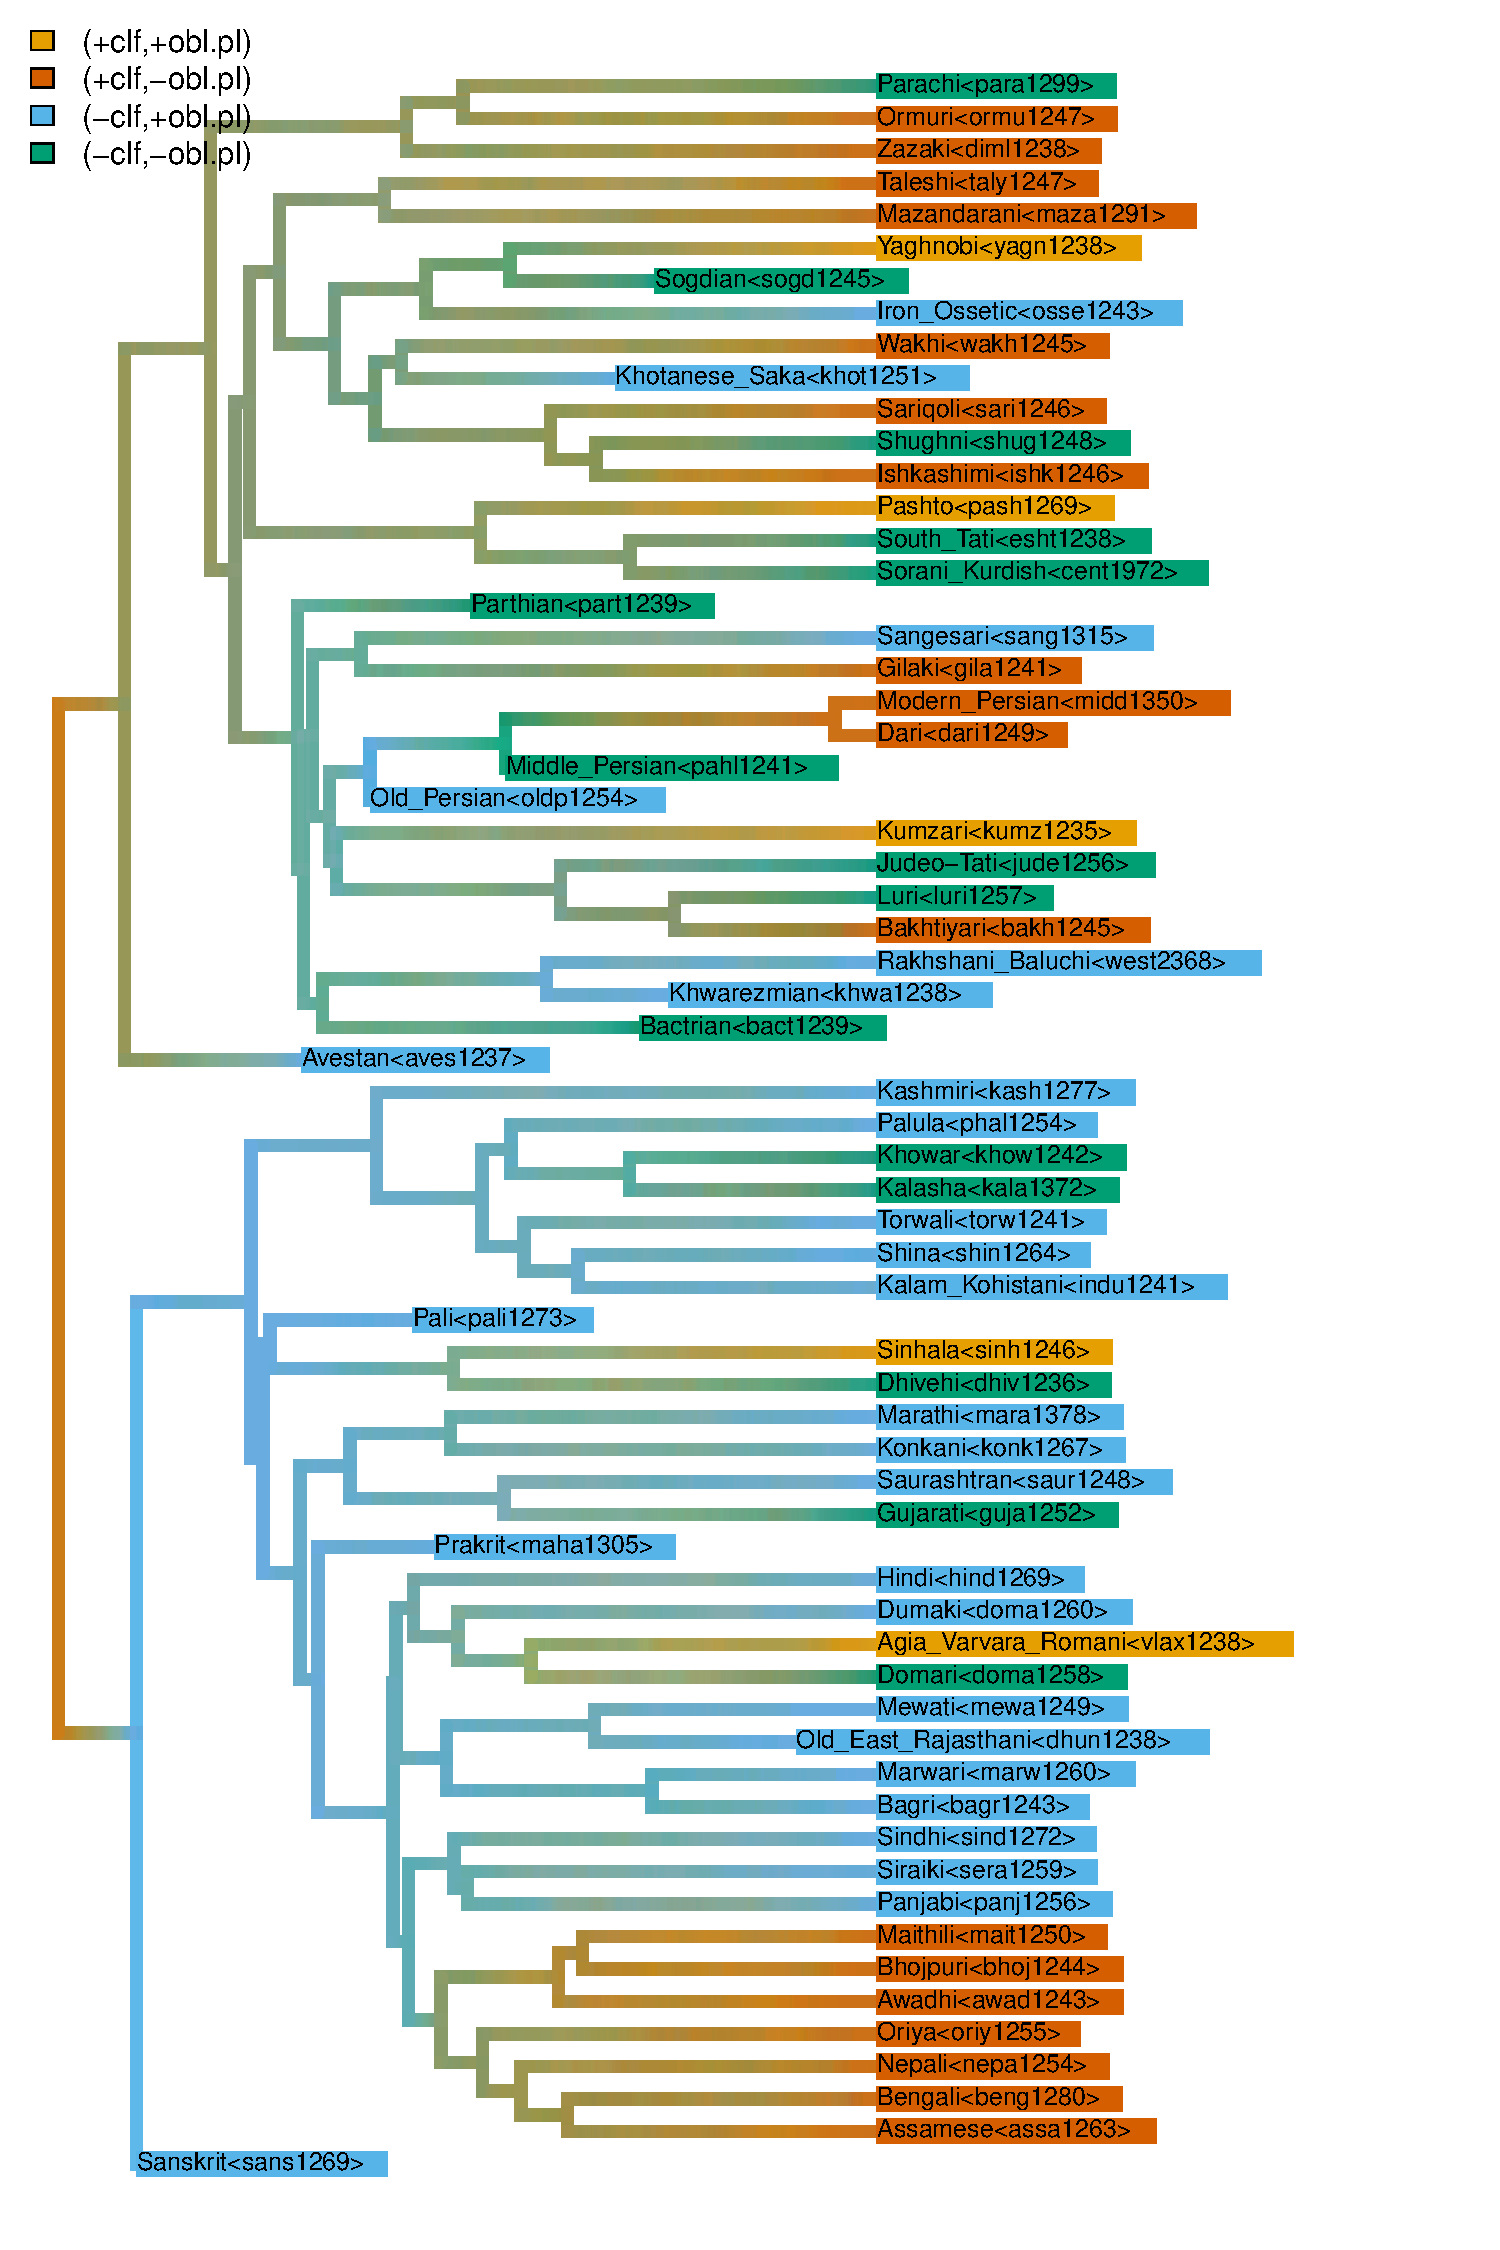
\includegraphics[width=.7\linewidth]{density_map.pdf}
\caption{Density map aggregating probable character histories over maximum clade credibility tree constructed from the tree sample.}
\label{densitymap}
\end{figure}


\begin{figure}[h!]
\centering
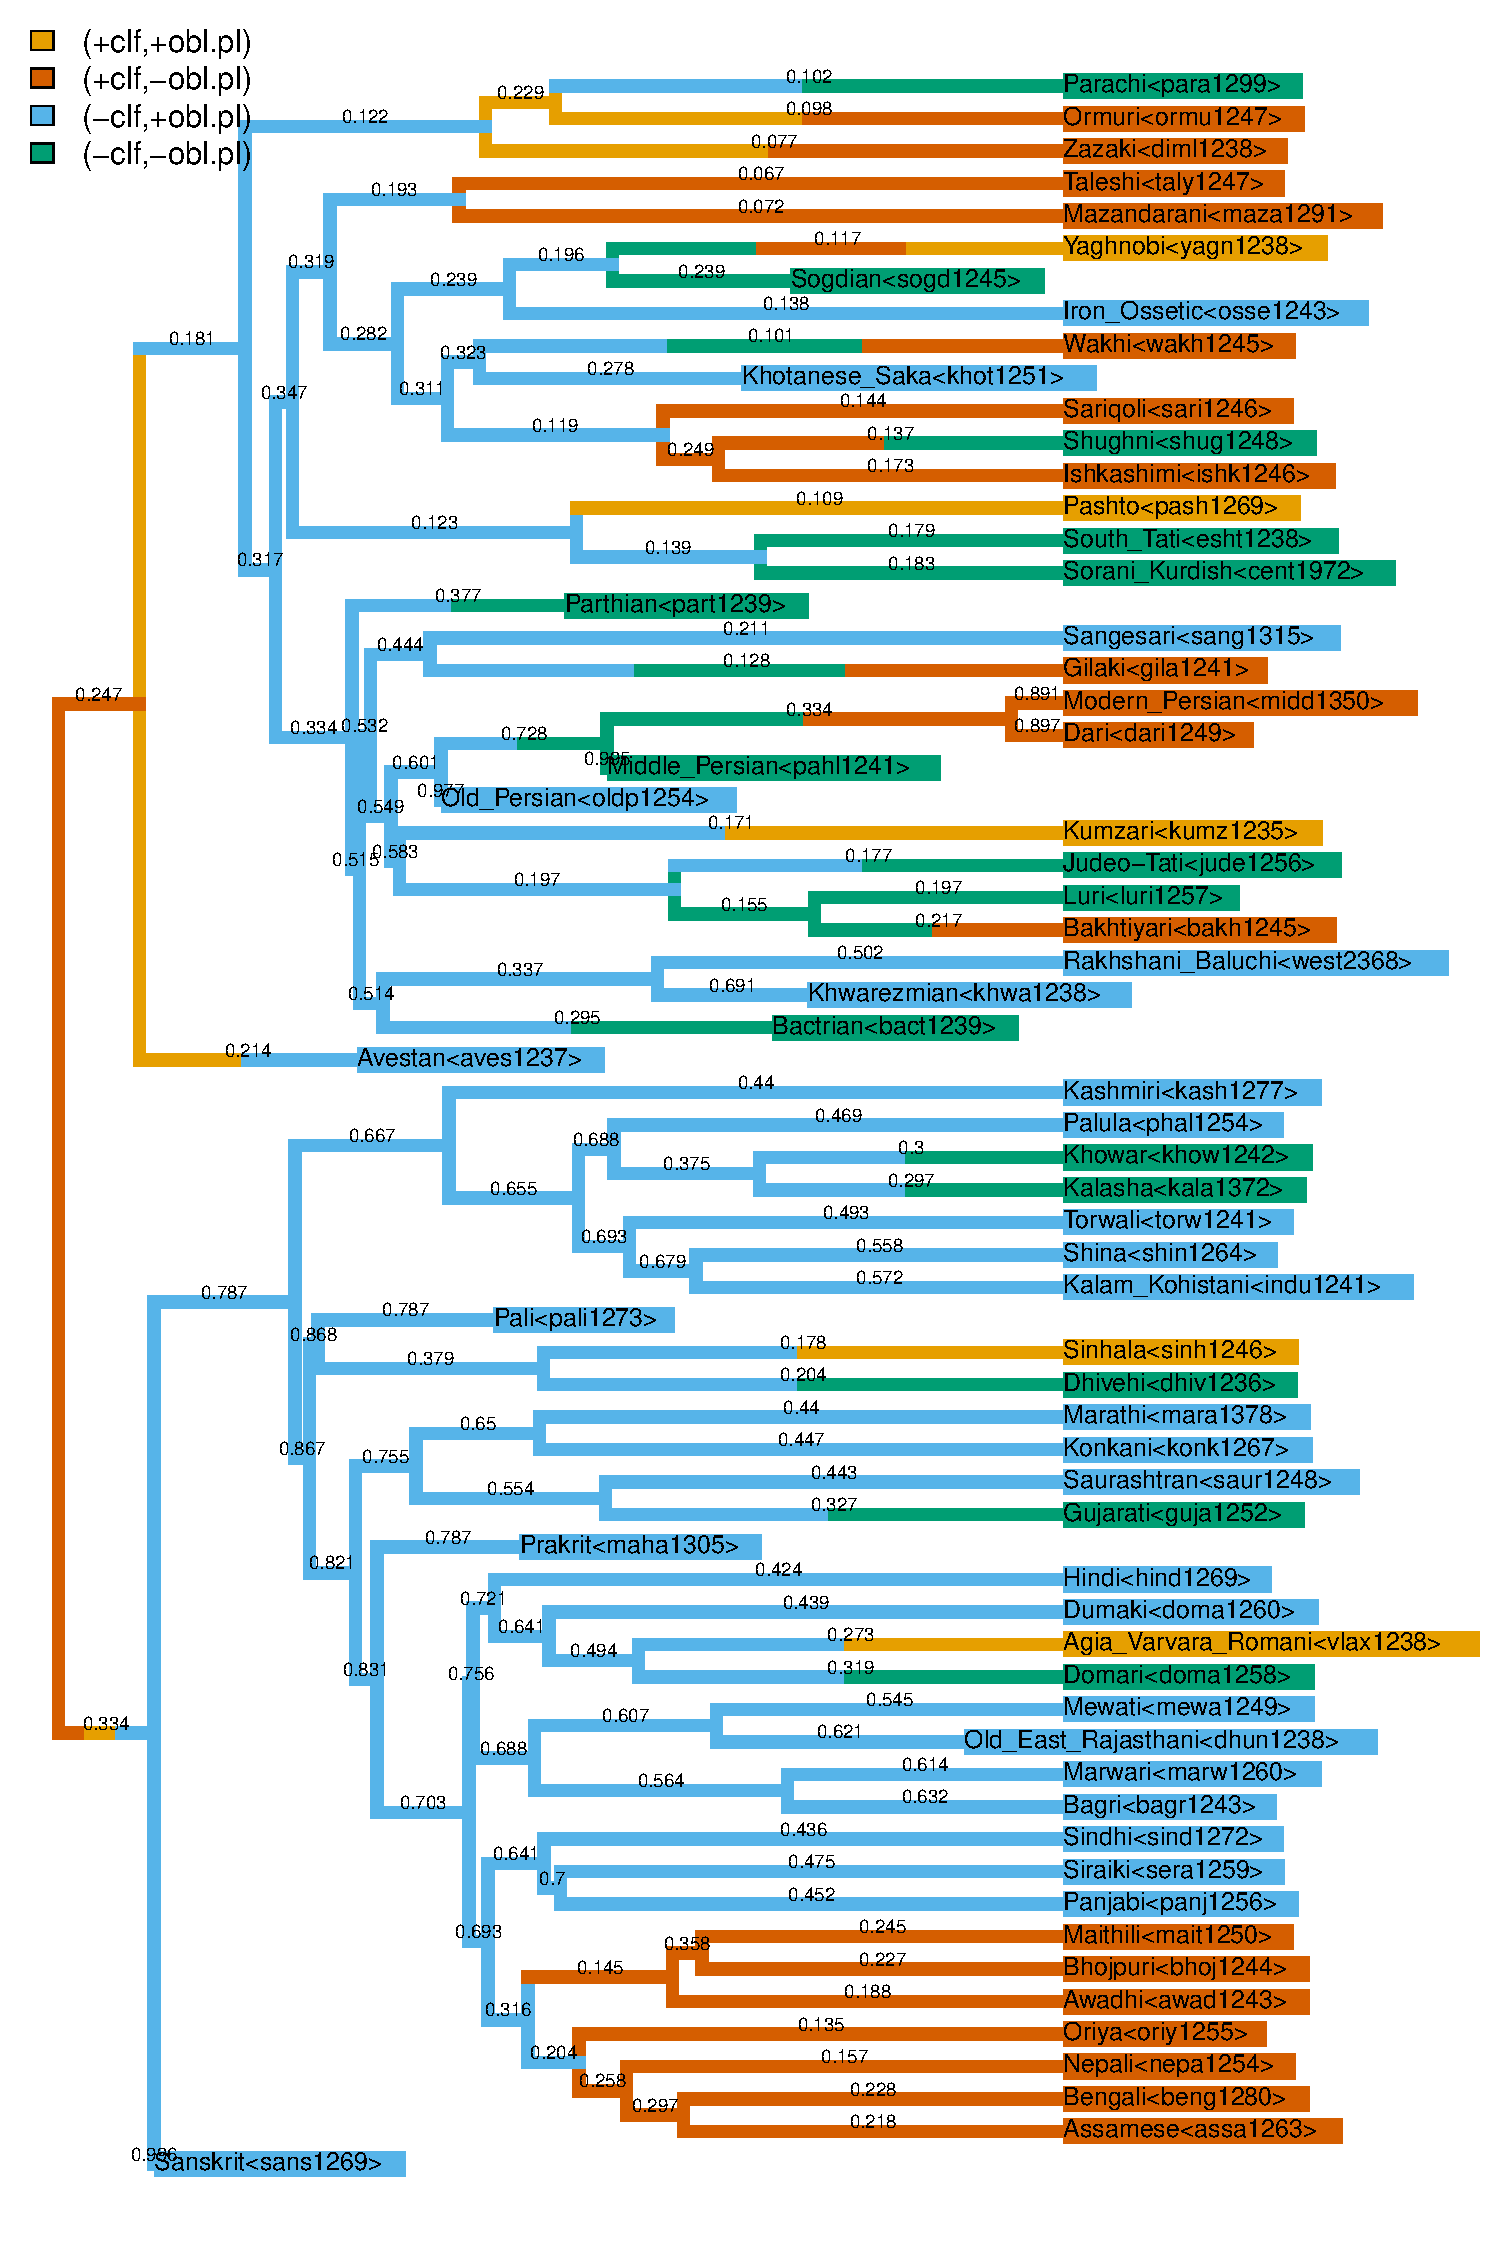
\includegraphics[width=.7\linewidth]{consensus_simmap.pdf}
\caption{MAP character history over maximum clade credibility tree constructed from the tree sample.}
\label{MAP}
\end{figure}

We carry out stochastic character mapping using the SIMMAP method \citep{Bollback2006} as implemented in the {\tt R} package {\tt Phytools} \citep{Revell2012}. We simulate character histories on the tree over 1000 iterations, drawing from the posterior sample of transition rates. 
The standard way for visualizing the aggregation of these histories is to use a density map, which represents the probability of a state in continuous space over the tree using a color gradient. Visualization can be a challenge for more than two states, since colors can become muddy in regions where uncertainty over the state value of the character is high. For this reason, we estimate a maximum a posteriori (MAP) character history over the tree by tabulating for each branch the counts for each type of transition history (ignoring the actual waiting times between transitions)
%{\color{red} irrespective of the times} at which each change occurs, 
and taking the most frequent transition history. 

We give both a density map and a MAP character history in Figures \ref{densitymap}--\ref{MAP}. Each branch is annotated according to the posterior support for its MAP transition history. 
%This procedure also allows us to estimate the probability of that a given state is present at each internal node of the tree, i.e., nodes in our tree where data are not observed. 
Striking differences in diachronic behavior between Indo-Aryan and Iranian can be observed. % in Figures \ref{densitymap}--\ref{MAP} 
In Indo-Aryan, classifiers emerge only three times (on branches ancestral to Sinhala, Agia Varvara Romani, and several Eastern Indo-Aryan languages), and their development is not preceded by a period of optional plural marking. 
In contrast, an overwhelming number of cases of classifier development in Iranian are preceded by periods of optional plural marking. 

To ensure that these patterns (and specifically, this difference across the two subgroups) is not simply an artifact of the topology of the maximum clade credibility tree, we carry out SCM on 1000 trees drawn from the tree sample, tabulating the number of times classifiers are gained in the presence of optional plural marking versus obligatory plural marking within Indo-Aryan and Iranian. 
The results of this procedure, shown in Figure \ref{ia_ir_scm}, indicate that for Iranian languages, classifiers develop more frequently in the presence of optional plural marking than in Indo-Aryan languages. 
Additionally, for each language with numeral classifiers, we note the most frequent state that preceded the development of classifiers in the lineage directly ancestral to the language. 
There are some discrepancies between the information presented in Figure \ref{MAP} and Table \ref{prev_state}; in many cases, the most frequent character history is outnumbered by non-identical character histories that all show the same state directly preceding the development of numeral classifiers --- for instance, the most frequent distinct character history on the branch leading to Sinhala is ($-${\sc clf}, $+${\sc obl.pl}) $\rightarrow$ ($+${\sc clf}, $+${\sc obl.pl}), but this trajectory is outnumbered by character histories that differ from each other but all show the state ($-${\sc clf}, $-${\sc obl.pl}) directly anterior to the state ($+${\sc clf}, $+${\sc obl.pl}) displayed by Sinhala. 
Furthermore, these relative frequencies do not always sum to one, since in a very small number of simulations, classifiers have been reconstructed at the root of the tree, and 
on certain lineages, states with classifiers are not preceded by states without classifiers. 
%on certain lineages, classifiers will be lost and regained, but on others, there is no {\tt previous state} lacking classifiers. 

\begin{figure}[t!]
%\begin{adjustbox}{max totalsize=\linewidth}
%\input{hypothesis_rates}
%\end{adjustbox}
\begin{minipage}[t]{.45\linewidth}
\includegraphics[width=\linewidth]{ia_transitions.pdf}
\end{minipage}
\hspace{.05\linewidth}
\begin{minipage}[t]{.45\linewidth}
\includegraphics[width=\linewidth]{iran_transitions.pdf}
\end{minipage}
\caption{Number of gains of numeral classifiers in the presence of optional versus obligatory plural marking for Indo-Aryan and Iranian over 1000 iterations of SCM.}
\label{ia_ir_scm}
\end{figure}


\begin{table}[h!]
\centering
\begin{tabular}{|l|ll|}
\hline
 & ($-$clf,$-$obl.pl) & ($-$clf,$+$obl.pl)\\
\hline
Assamese$*$ & 0.379 & 0.621\\
Bengali$*$ & 0.379 & 0.621\\
Oriya$*$ & 0.387 & 0.613\\
Awadhi$*$ & 0.387 & 0.613\\
Nepali$*$ & 0.383 & 0.617\\
Bhojpuri$*$ & 0.385 & 0.615\\
Maithili$*$ & 0.391 & 0.609\\
Agia Varvara Romani$\dagger$ & 0.496 & 0.504\\
Sinhala$*$ & 0.535 & 0.465\\
\hline
Ishkashimi$*$$\dagger$ & 0.799 & 0.2\\
Sariqoli$*$$\dagger$ & 0.751 & 0.248\\
Wakhi$\dagger$ & 0.643 & 0.356\\
Yaghnobi$\dagger$ & 0.78 & 0.22\\
Pashto$\dagger$ & 0.621 & 0.379\\
Mazandarani$*$$\dagger$ & 0.725 & 0.274\\
Taleshi$*$$\dagger$ & 0.729 & 0.271\\
Bakhtiyari$*$ & 0.685 & 0.315\\
Dari$*$$\dagger$ & 0.944 & 0.056\\
Modern Persian$*$$\dagger$ & 0.951 & 0.049\\
Kumzari$*$ & 0.593 & 0.407\\
Gilaki$*$$\dagger$ & 0.602 & 0.398\\
Zazaki$*$$\dagger$ & 0.714 & 0.286\\
Ormuri$*$$\dagger$ & 0.719 & 0.281\\\hline
\end{tabular}
\caption{Relative frequencies of states directly preceding the development of classifiers in lineages of languages with classifiers, averaged over 1000 SCM iterations.}
\label{prev_state}
\end{table}

Ultimately our results show that the GSS has considerable explanatory power regarding the development of classifiers in Indo-Iranian, but it is clear that classifier development is not solely a response to optional plural marking. While most of the developments seen in Iranian are largely compatible with the GSS generalization, this is not the case for Indo-Aryan. 
In the following section, we analyze the developments shown above individually, assessing the role of different factors potentially underlying the development of numeral classifiers in Indo-Iranian speech varieties. 


\section{Discussion}
Overall, our results show that the GGS may account for a considerable number of incidences of classifier development in Indo-Iranian, but suggest that other factors such as contact may play a role as well, and furthermore that there may be some degree of interaction between these factors. 
When discussing areal effects, we draw a simple distinction between cases in which Indo-Iranian languages have participated in prestige-driven borrowing of classifiers, and cases where Indo-Iranian languages have taken on patterns of classifier use and/or number marking under circumstance of stable multilingualism. This framework suits the purposes of our paper's analysis, but draws upon larger theories of source/recipient agentivity \citep{Ross1996,Winford2005,MatrasSakel2007}. 
In this section, we integrate our model results with qualitative insights regarding Indo-Iranian contact history in order to sketch a plausible account of the development of classifiers across the subgroup. 

\paragraph{Indo-Aryan}
A striking aspect of the character history that we have inferred over the tree is that in Indo-Aryan languages, classifiers come about far less frequently than they do in Iranian. It is likely that a single development accounts for the presence of classifiers across Eastern Indo-Aryan. 
In each case of emergence, classifier development does not appear with high certainty to be preceded by a period of optional plural marking, counter to the GSS hypothesis.\footnote{The figures in Table \ref{prev_state} show that the state ($-${\sc clf}, $-${\sc obl.pl}) precedes the development of classifiers in these two languages in roughly 50\% of SCM iterations. This value is lower than what we expect, and may be an artifact of the exclusion of additional Romani varieties (where plural marking is obligatory) and data, however incomplete, from Old Sinhala (see below).} 
This state of affairs seems to favor language contact as a potential explanation; however, matter borrowing has taken place in only one Indo-Aryan language with classifiers: 
Agia Varvara Romani has clearly borrowed {\it tane} from Turkish (see above), likely due to the prestige of the latter language; this element is found in other Romani dialects in contact with Turkish \citep[204]{Matras2002}. 

%Sinhala
Unlike Agia Varvara Romani, the Sinhala classifier is inherited, and does not point explicitly to contact. 
Our model's results do not provide much information as to whether Sinhala developed classifiers in the presence of optional plural marking. 
Given the historical record, this seems unlikely; 
Modern Sinhala obligatory number marking is thought to have developed from an earlier stage where singular marking was non-obligatory \citep{NitzNordhoff2010}.\footnote{While it is not possible from the available historical record to date the development of the {\it denaa} classifier relative to the development of a more restrictive number marking system, it is possible that the former development took place while singular marking still exhibited a degree of optionality. Either way, neither a system with obligatory number marking nor a system with optional singular marking should give rise to numeral classifiers under the Greenberg-Sanches-Slobin hypothesis.} 
Incidentally, the Sinhala classifier construction is very similar to that of surrounding Dravidian languages, especially Tamil.  Sinhala {\it denaa} apparently still has its meaning `people' in other contexts \citep[passim]{Chandralal2010}. 
In Modern Literary Tamil \citep[112--114]{Lehmann1993}, numerals above one have a so-called pronominalized form with a suffix {\it -ar}. In Modern Spoken Tamil \citep[132--135]{Schiffmann1999}, pronominalized numerals higher than one add the noun {\it peeru} `name' instead, which can also mean `person'. In both languages the newly formed numeral can be used attributively or pronominally. If used attributively, it can precede or follow the head noun. In Literary Tamil, they have a marked genitive reading instead if preposed. In Spoken Tamil, they have a specific or definite reading if postposed. The similarities with Sinhala are striking. In all three languages there is [N [Num Clf]] word order as at least one possibility and there is a connection with animacy, non-animate or non-human entities being unmarked. Some Dravidian languages on the mainland have similar classifier-like constructions for humans. In Telugu, for instance, numerals above eight combine with the word {\it mandi} `persons', e.g. {\it padi-mandi} `ten persons' \citep[106--109]{KrishnamurtiGwynn1985}. %Because Sinhala {\it denaa} is cognate with classifiers in other Indo-Iranian languages, there is also the possibility that the construction is a retention in Sinhala that influenced the Dravidian languages of the area. 
%However, the direction of influence is not altogether clear. 
%More historical and diachronic research is necessary to clarify this point.

The diachrony of the development of numeral classifiers in Eastern Indo-Aryan languages like Bengali is poorly understood. There is some evidence that medieval East Indo-Aryan languages had optional plural marking. \citet[23]{Mukherji1963} states that Old Bengali lacks morphological number, but that ``plurality ... can be expressed by combining a singular noun with a number of words which denote plurality.'' It is not clear whether this feature co-existed with classifier use, as there is good reason to believe that this feature was suppressed in literary registers, our only source of data on languages of this sort \citep[cf.][]{BarzDiller1985}. 
If the historical scenario suggested by our results is accurate, a sweeping change of the type {\sc ($-$clf, $+$obl.pl)} $\rightarrow$ {\sc ($+$clf, $-$obl.pl)} took place in the history of Eastern Indo-Aryan. This development suggests a change in the general typological profile of these languages, possibly brought about by widespread language shift. 

Eastern Indo-Aryan languages with numeral classifiers are spoken in the vicinity of Dravidian (e.g., Kurux), Austroasiatic (especially Munda, e.g. Kharia), and Sino-Tibetan (especially Tibeto-Burman, e.g., Jero) languages, many of which also exhibit numeral classifiers. 
%The most likely explanation is an areal connection between these languages. Although it is often difficult to identify the exact pattern of diffusion, there are many clear cases of borrowing. Consider the following data.
%\begin{example} Kharia (Austroasiatic)
%\gll tin jhan lebu=ki
%three {\sc clf} person={\sc pl}
%\glt `three people' \citep[195]{Peterson2011}
%\glend
%\end{example}
%\begin{example} Kurux (Dravidian)
%\gll du{\IPA :}-{\IPA \:t}hu{\IPA :} xadd-ar
%two-{\sc clf} children-{\sc pl.hum}
%\glt `two children' \citep[114]{KobayashiTirkey2017}
%\glend
%\end{example}
%\begin{example} Jero (Sino-Tibetan)
%\gll dui g{\IPA O\:t} mi
%two {\sc clf} fire
%\glt `two fires' \citep[118, shortened]{Opgenort2005}
%\glend
%\end{example}
%Similar to the situation in Iranian, it is paradoxically often the Indo-Aryan numeral classifier system that is adopted by surrounding languages instead of the other way around. Kharia {\it jhan} derives from Sadri \citep[195]{Peterson2011}, Kurux {\it {\IPA \:t}hu{\IPA :}} from Bihari \citep[305]{KobayashiTirkey2017}, and Jero {\it g{\IPA O\:t}} from Nepali \citep[117]{Opgenort2005}. In both cases, Iranian and Indo-Aryan, one possible explanation for the unexpected pattern could be a substrate influence that might have led to the emergence of numeral classifiers based on autochthonous Indo-Iranian material (pattern borrowing). 
%Subsequently, because of the larger number of speakers and the higher prestige of Indo-Iranian languages, some of these numeral classifiers have been adopted by surrounding languages, often in combination with the Indo-Iranian numeral system (matter borrowing). Because of this, in several languages the autochthonous numerals and classifiers are restricted in use or have been entirely lost. For example, the Sino-Tibetan language Yakkha has borrowed the Nepali numeral system and only retains the autochthonous numerals from one to three, although the Nepali numeral for one is also employed. Today, the human numeral classifier {\it -pa{\ng}} can only be combined with the Yakkha numerals two and three \citep[105--106]{Schackow2015}. 
%Exactly the same pattern is observed in Belhare (as cited above). 
%
%Due to the large number of numeral classifiers and its eastern location, {Assamese} represents a special case among the Eastern Indo-Aryan languages. \citet[48--51]{Moral1997} has given conclusive evidence for the scenario that the Assamese numeral classifier system has been heavily influenced especially by Tibeto-Burman languages. Contact languages of Assamese include Sino-Tibetan (e.g., Bodo, Garo, Meche), Kradai (e.g., Khamti), and Dravidian languages (e.g., Malto). The Meche language, for example, exhibits a large amount of numeral classifiers, only some of which have been adopted from Nepali \citep[17--19]{Kiryu2008}. Among Dravidian languages, the largest inventory of numeral classifiers can be found in Malto that is also spoken in the vicinity of Assamese \citep[128--132]{Mahapatra1979}. 
%A large number of numeral classifiers are also present in the Kradai language Khamti.
Striking parallels with the behavior of East Indo-Aryan classifiers can be found in the Kradai language Khamti. 
In Khamti, [N Clf Num] word order has an indefinite reading with the numeral `one', while [N Num Clf] word order is definite. 
Interestingly, Assamese, Bengali, and Oriya have a connection of word order with definiteness, where [N Num Clf] word order is definite while [Num Clf N] order is indefinite. 
% BB: I think to make this relevant, we need to cite an IA example with the same word order effect.
%CC: added
\begin{example} Khamti (Kradai)
\gll kuun\textsuperscript{4}maau koo\textsuperscript{1} leeung\textsuperscript{3}
bachelor {\sc clf} one
\glt `a bachelor' \citep[8, shortened]{Inglis2007}
\glend
\end{example}
\begin{example}
\gll kuun\textsuperscript{4} saam koo\textsuperscript{1}
person three {\sc clf}
\glt `three people' \citep[11, shortened]{Inglis2007}
\glend
\end{example}
\begin{example} Bengali
\gll ch{\IPA O} -\d{t}a boi
six {\sc -clf} book
\glt `six books' \citep[136]{David2015}
\glend
\end{example}
\begin{example}
\gll boi ch{\IPA O} -\d{t}a
book six {\sc -clf}
\glt `the six books' \citep[137]{David2015}
\glend
\end{example}
While further parallels and matches in morphosyntactic pattern are needed in order to make a conclusive case for a shift from a language specifically like Khamti to Eastern Indo-Aryan, the striking differences from other Indo-Aryan languages, as well as the dynamics of change shown in the evolutionary scenario that we infer, lend support to the idea that the typological profile of Eastern Indo-Aryan languages is due to contact rather than diachronic trends realized elsewhere in Indo-Iranian.


\paragraph{Iranian}
In contrast to the situation in Indo-Aryan, 
Iranian languages on the other hand appear to have developed classifiers more frequently; classifiers emerge on nine independent branches within Iranian. 
The majority of these developments are preceded by stages with optional plural marking; ultimately, the state of affairs characterized by the GSS generalization appears to have been more active in Iranian than in Indo-Aryan, although if cognitive pressure is largely responsible for the development of classifiers in Iranian, it most likely interacted with areal pressure (both in the form of prestige borrowing and multilingualism), leading to the spread of this feature across languages. 

%\subparagraph{Persian}
The historical record makes it relatively clear that the development of full-fledged numeral classifiers in Persian was preceded by a prolonged period of optional plural marking, a state of affairs recapitulated by our SCM procedure. Our evolutionary model suggests that this was the case on branches leading to Wakhi; the Pamir languages Sariqoli, Shughni and Ishkashimi; Taleshi; and Kumzari as well. Hence, these developments are compatible with the claims made by the GSS hypothesis. However, contact may have also played a role; the proximity of Iranian languages to Turkic languages possessing classifiers cannot be ignored. 
As mentioned previously, Turkic and Iranian languages came increasingly into contact in post-Sasanian times. 
However, numeral classifiers are a likely to be a relatively late development, post-dating the onset of the Turkic expansion from about the 5th century CE \citep{Yunusbayev2015}. The Old Turkic (ca. 7th to 11th century) corpus contains no sortal numeral classifiers \citep[226]{Erdal2004}; however, the later literary language Chagatay (ca. 14th to 19th century) in Central Asia already exhibited certain classifiers, such as {\it ba\v{s}} `head' \citep[155]{Bodrogligeti2001}, and classifier use in modern Turkic languages is widespread, found among different branches of Turkic, including Kipchak (e.g., Tatar, \citealt[70]{ChenZongzhenYiLiqian1986}), Oghuz (e.g., Turkmen, \citealt[169]{Clark1998}), and Karluk (e.g., Uzbek, \citealt{Beckwith1998}). 
It is not clear whether this distribution reflects a widespread, relatively late diffusion of the feature under question throughout Turkic or the realization of some sort of drift or slant-like tendency on one hand, or the inheritance of a chronologically deep feature within the Turkic family. 
Complicating matters, Turkic classifiers are often Iranian loans; only in restricted occurrences do Iranian languages borrow Turkic classifiers (e.g., Sariqoli $\leftarrow$ Uyghur). 
Further research and more methodological development is needed to address the question of whether Turkic classifiers are due to Iranian influence, Iranian classifiers are due to Turkic influence, or both groups developed classifiers as a response to loosening restrictions on plural marking under the influence of widespread multilingualism. 

%\subparagraph{East Iranian}
In some cases, the presence of numeral classifiers in Iranian languages is clearly due to influence from other Iranian languages. 
The numeral classifiers found in Wakhi, Yaghnobi and certain Pamir languages are clearly identifiable as Tajik, given Tajik's importance as a lingua franca in the region where these languages are spoken. 
Pashto has likely borrowed the classifier {\it tana} (m.)/{\it teni} (f.) from a Turkic language, though it has been in the language long enough to be integrated into the gender system and participate in a phonological process. 

%\subparagraph{Kumzari}
In other cases, the role of contact is unclear. Kumzari, located in Oman and is separated from other Iranian languages by the Persian Gulf, exhibits the classifiers {\it -ta} and {\it -kas} (for human beings), formally identical to the Persian classifier {\it t\=a} and the Persian word {\it kas} `person'. Kumzari is genetically very close to Old, Middle, and modern Persian \citep{Skjaervo1989b}, though it is not clear that it is a descendant of Old or Middle Persian. Given the relative isolation of Kumzari, it is possible that it developed these classifiers in parallel with Persian due to drift, %(i.e., because an incipient tendency toward close nominal apposition )
but contact with another Iranian language is also a possibility, since there has been longstanding migration to Oman from the other side of the Persian Gulf \citep{Barth1983}.\footnote{Though the historical phonology of Kumzari is poorly understood, there is some evidence that it preserves the consonant of Old Iranian final {\it *-aka-}, given the ``etymologically latent {\it k}'' in the definite form {\it martk-\=o} \citep[38]{WalAnonby2015} $<$ {\it *marta-ka-}. Modern Persian does not preserve this consonant (cf. {\it t\=a} $<$ Middle Persian {\it t\=ag} `piece', most likely going back to an element {\it *t\=aka-}). However, Kumzari seems to show preservation only in contexts where the form is suffixed, making it impossible to determine whether the loss of {\it -k} in {\it -ta} is regular or reflects a Persian borrowing.} 
Under our phylogenetic model, there is approximately 60\% posterior probability that Kumzari developed the state ($+${\sc clf}, $+${\sc obl.pl}) after a stage of optional plural marking (see Table \ref{prev_state}); the development of obligatory plural marking may be due to contact with neighboring Arabic, which has obligatory plural marking. 

The remainder of Iranian languages with classifiers (e.g., Mazandarani, Taleshi, and Gilaki) share a core group of classifiers that are formally near-identical to Persian ones (e.g., {\it t\=a}), but as in the case of Kumzari, %it is challenging to invoke Persian contact 
%{\tt }
%there is no explicit evidence for Persian contact in the form of 
%sound change, 
it is difficult to determine whether these forms are inherited or borrowed on the basis of sound change; 
at the same time, the dominance of Persian  over these languages is well established \citep{Borjian2009}, lending circumstantial evidence to the notion that they are Persian loans. 
Some Northwest Iranian languages have classifiers not found in Persian, e.g., Taleshi {\it g{\textschwa}la} \citep{Paul2011,Stilo2018}, perhaps cognate to Judeo-Tati {\it gile} `time, instance' \citep[310]{Authier2012}. 
Many of these languages appear to have undergone a long-term trend toward optional plural marking. It is likely that classifiers spread through contact, but did so because of their utility and the cognitive enhancement they brought about. 

%{\tt possible that they caught on because they were beneficial and due to prestige language}.

%Unless this represents a later diffusion of the feature under question throughout Turkic or the realization of some sort of drift or slant-like tendency, these facts suggest a relatively early emergence of classifiers in Turkic even before the literary Chagatay language. Some Turkic languages, such as Uzbek \citep{Beckwith1998} or Uyghur \citep{TuohutiLitifu2012}, exhibit several numeral classifiers. Paradoxically, many of the numeral classifiers in Turkic languages represent borrowings from Iranian languages. For example, the classifiers {\it d\^ana} in Uzbek \citep[131]{Beckwith1998} and {\it dan\"a} in Uyghur derive from Iranian and usually combine with inanimate objects (e.g., book, car, house, pen, TV, watermelon, \citealt[158f.]{TuohutiLitifu2012}). In the Turfan dialect of Uyghur, {\it dan\"a} also combines with animate and human nouns (e.g., cow, grandchild, soldier, \citealt[107, 173]{Yakup2005}).

From the evidence surveyed, a picture emerges where in the majority of cases, Indo-Iranian classifiers developed as both a response 
to the individual effects of contact and optional plural marking, and likely via an interaction between the two. Iranian languages often use borrowed matter as numeral classifiers, regardless of whether plural marking is optional or obligatory, as shown in Table \ref{counts}. In some cases actual classifiers are borrowed (e.g., Zazaki {\it teney} from Turkish); in others, borrowed matter seems to have been repurposed as classifiers (e.g., Persian uses Arabic loanwords as classifiers in addition to inherited material, though they probably did not enter the language as such). 
However, Iranian languages with obligatory plural marking seem not to have developed classifiers from inherited matter. 
Yaghnobi has borrowed classifiers from Tajik. 
The case of Kumzari is ambiguous, as it is not clear whether its classifiers are Persian cognates or loans, or whether plural marking was obligatory in Kumzari when classifiers developed. 
With the exception of Romani dialects, Indo-Aryan languages appear to have taken on patterns of number marking and classifier use from neighboring languages of other stocks (e.g., Kradai and Dravidian). 
 
 
\begin{table}
{\small 
 \begin{tabular}{|p{.15\linewidth}||p{.25\linewidth}|p{.25\linewidth}|p{.25\linewidth}|}
 \hline
% \hline
  & Borrowed matter & Inherited & Both \\
 \hline
% \hline
 +clf,-obl.pl & Wakhi & Bhojpuri, Awadhi, Maithili, Nepali, Oriya, Bengali, Assamese, Bakhtiyari & Sariqoli, Ishkashimi, Zazaki, Modern Persian, Dari, Gilaki, Taleshi, Mazandarani, Ormuri \\
\hline
+clf,+obl.pl & Agia Varvara Romani, Pashto, Yaghnobi & Sinhala, Kumzari & \\
\hline
 \end{tabular}
 }
 \caption{Table showing whether numeral classifiers are based on borrowed or inherited matter in languages with numeral classifier systems.}
 \label{counts}
 \end{table}

%I think we can make the following argument: in the majority of cases, classifiers developed as both a response to optional plural marking *and* contact, and this was realized both by means of pattern and matter borrowing. In the Indo-Aryan pattern borrowing case, prestige was likely not a factor. For Iranian languages with (+clf,-obl), prestige may have been a factor in some isolated cases. Prestige borrowing is almost certainly responsible for the presence of classifiers in Ajia Varvara Romani, Yaghnobi, and perhaps Pashto, which have (+clf,+obl), but not for Sinhala, and it is not clear what is going on in Kumzari. Hence, classifier borrowing overwhelmingly serves to bring about cognitive benefits, but in the majority of the few cases where it does not bring about cognitive benefits, it tends to be due to emblematic pressure from a prestige language.

{\color{green} Ultimately, languages with non-obligatory plural marking have classifiers based on either inherited or borrowed matter, but languages with obligatory plural marking tend to have classifiers based {solely} on borrowed matter (except for Sinhala and maybe Kumzari). If languages of the latter type borrowed classifiers during a stage when plural marking was not optional, it was possibly because the prestige of the source language trumped the fact that numeral classifiers would bring no understandable cognitive benefit to a language with obligatory plural marking. 
Languages where the development of classifiers brought about a cognitive benefit as well may have borrowed their classifiers from source languages with and without relative prestige, and this is reflected by the combination of matter (pointing to prestige) and pattern (pointing to stable multilingualism) borrowing that they display. 
Further research at a wider phylogenetic scale is needed to conclusively address some of these questions.
Use of phylogenetic models designed to account for heterotachy (evolutionary rates that vary between different regions of the tree) may help to better capture clade-specific diachronic preferences, though our results show a clear difference in the evolutionary behavior of Indo-Aryan and Iranian without such a model.}


\section{Conclusions}
\label{conc}
Our findings suggest that the emergence of classifiers is often tied to optional plural marking, partially explainable by a statistical universal principle in line with the Greenberg-Sanches-Slobin generalization. 
At the same time, we find that classifiers emerged specifically under contact, reflecting local history and the contingencies of migration and trade. These results seem contradictory when one approaches the distribution of linguistic structures from the popular view that conceptualizes universal pressure and areal histories as conflicting, confounding, and competing factors. The contradiction is resolved, however, if we adopt the view from Distributional Typology \citep{Bickel2015Distributional} where emphasis is placed on the \emph{interaction} between universal and areal factors \citep{Bickel2014Areas}. 

From this perspective, the borrowing of classifiers (as matter or pattern) is not the mere product of historical contingency. Instead, this borrowing is driven by the decay in number marking, i.e. it follows the Greenberg-Sanches-Slobin generalization. Such a scenario explains our finding that classifiers were considerably more likely to be borrowed in the absence than in the presence of number marking. Areal effects alone cannot explain this difference, while universal effects alone cannot explain why classifiers entered through borrowing rather through spontaneous developments (e.g.\ by reanalyzing nominal juxtapositions, as in Hackstein's \citeyear{Hackstein2010} theory).

While our study supports a scenario of an interaction between universal and areal effects, we caution that our simplified coding scheme may not have picked up all relevant factors and that further research is needed to consolidate our conclusions. What is arguably the most urgent extension is a more fine-grained coding that captures the distribution of number marking over specific noun types, controlling for potential effects of a referential scale.



}



\bibliographystyle{chicagoa}
\bibliography{pre_pilot_bibliography}

\paragraph{Agia Varvara Romani [vlax1238] (+clf,obl.pl)}
Singular forms are always morphologically distinct from their plural counterparts, usually via the addition of a plural suffix or alternation of the final vowel \citep[23ff.]{Igla1996}. When a numeral greater than one modifies a noun, the noun is morphologically plural (p.\ 45). When the counted item consists of indefinite objects, then {\it -tane} ($<$ Turkish {\it tane} `piece, part') appears next to the numeral; anaphoric use of this classifier is obligatory (p.\ 45). 
\paragraph{Assamese [assa1263] (+clf,opt.pl)}
Assamese has a large inventory of sortal classifiers. Plural marking is optional \citep{Borah2012,Chowdhary2012}.
\paragraph{Avestan [aves1237] (-clf,obl.pl)}
Plural number is consistently marked, given rich agreement morphology \citep{HoffmannForssman2002}.
\paragraph{Awadhi [awad1243] (+clf,opt.pl)}
Classifiers are present; information regarding plural marking is difficult to extract from \citealt[115ff.]{Saksena1971}, but it appears to be optional.
\paragraph{Bactrian [bact1239] (-clf,opt.pl)}
In late Bactrian, case and number distinctions have been neutralized due to the loss of distinctions between final vowels, resulting in ``an unmarked form without ending ... which may be used with either sg. or pl. reference, and a marked pl. form'' \citep[40]{SimsWilliams2007}.
\paragraph{Bagri [bagr1243] (-clf,morph.pl)}
There are at least three declensional classes, in one of which the plural and singular direct forms are identical. The distinction between animacy and inanimacy, rather than ending in {\it -i} versus other segments, is made by the author, who explicitly states that the suffix {\it -\~{a}} is optional on animate nouns. This is almost akin to a mixture of a system like that of Hindi, where plural cannot be marked on some noun case forms, and a system where plural marking is truly optional.
\paragraph{Bakhtiyari [bakh1245] (+clf,opt.pl)}
Classifiers are present, and plural marking is variable \citep{AnonbyAsadi2014}.
\paragraph{Bengali [beng1280] (+clf,opt.pl)}
Bengali has a large repertoire of numeral classifiers \citep[135]{David2015}. Classifiers are obligatory with non-numeric quantifiers and lower numbers; optional with numbers ending in `hundred', `thousand', `lakh', etc. (p. 142). Numeral classifiers cannot cooccur with nouns denoting a countable unit, e.g., units of weight, currency, time, except in certain emphatic contexts (p. 142). Plural marking is non-obligatory (p. 76).
\paragraph{Bhojpuri [bhoj1244] (+clf,opt.pl)}
Numeral classifiers are present, and plural marking is non-obligatory \citep[120, 228, 230]{Tiwari1960}
\paragraph{Dari [dari1249] (+clf,opt.pl)}
Classifier use is common, but not obligatory; plural marking is optional; it is not clear if plural marking can co-occur with classifier use as in Standard Modern Persian (\citealt[74-5]{Kiseleva1985}; \citealt[58-9]{Ioannesjan1999}).
\paragraph{Dhivehi [dhiv1236] (-clf,opt.pl)}
For nonhuman nouns, plural marking is optional when plurality is clear from context \citep[59]{Gnanadesikan2017}.
\paragraph{Domari [doma1258] (-clf,opt.pl)}
Plural marking on enumerated nouns interacts significantly with whether the numbers are inherited Indo-Aryan forms or borrowed from Arabic (see \citealt[97, 188ff.]{Matras2012}). Plural number is optionally marked on nouns modified by 2--3 (inherited numbers), obligatory on nouns modified by 4--10 (Arabic numbers), and optionally marked on nouns from 11 upward (Arabic numbers).
\paragraph{Dumaki [doma1260] (-clf,obl.pl)}
For virtually all nouns, the singular form is distinguishable from the plural form \citep[24ff.]{Lorimer1939}; this is achieved via suffixation or a stem alternation.
\paragraph{Gilaki [gila1241] (+clf,opt.pl)}
\citet{Rastorguevaetal2012} list several classifiers. Classifier use is optional when enumerating nouns, but appears to be quite common and obligatory in anaphoric use. In all examples given of counted nouns, there is no overt plural marking on the head noun (regardless of whether a classifier is present). Plural can otherwise be marked by means of certain suffixes.
\paragraph{Gujarati [guja1252] (-clf,opt.pl)}
\citet[66--7]{Cardona1965} refers to the plural marker {\it -o} as ``optional,'' and it seems to largely be omitted when nouns are modified by a number greater than 1; so-called ``variable'' nouns display a special ``dependent stem form'' when they are semantically plural, regardless of the presence of the suffix {\it -o}.
\paragraph{Hindi [hind1269] (-clf,morph.pl)}
Hindi shows four declensional classes; the details of number marking are different for each one. Certain noun types are paradigmatically non-exhaustive; plural marking not morphologically possible on C-final masculine nouns in direct case \citep{Oberlies2005}.
\paragraph{Iron Ossetic [osse1243] (-clf,obl.pl)}
Plural number is marked on nouns by means of the suffix {\it -t-} \citep[117]{Thordarson2009}. In most contexts (except for contexts of enumeration, see below), use of {\it -t-} appears to be obligatory. When a noun is enumerated by a numeral greater than one, the noun is marked by the suffix -i (Digor), identical to the genitive suffix. According to \citet[132]{Thordarson2009}, this suffix continues the Old Iranian plural suffix {\it *-ah}. Nouns enumerated by numbers greater than one are always marked in a way that renders them distinct from singular nouns.
\paragraph{Ishkashimi [ishk1246] (+clf,opt.pl)}
Ishkashimi contains at least three classifiers; nouns modified by a numeral greater than 1 can appear in singular or plural form \citep[50]{Paxalina1959}.
\paragraph{Judeo-Tati [jude1256] (-clf,opt.pl)}
Plural is marked on nouns with the suffix {\it -ho} \citep[79]{Authier2012}. Overt plural marking on enumerated nouns seems virtually non-existent.
\paragraph{Kalam Kohistani [indu1241] (-clf,obl.pl)}
Kalam Kohistani achieves plural marking on a number of nouns via a vowel fronting process, which also is found in oblique forms of nouns, and appears to mark plural consistently on nouns \citep[21]{BaartSagar2004}. The word {\it khur} `foot' may show variability in plural marking, but it is not clear from the data given.
\paragraph{Kalasha [kala1372] (-clf,opt.pl)}
Plural marking is optional \citep[35--6]{Petersen2015}.
\paragraph{Kashmiri [kash1277] (-clf,morph.pl)}
According to \citet[190ff.]{WaliKoul1996}: ``plurals are formed from singular stems by vowel change, palatalization and suffixation. A few nouns stay invariant. Masculine plurals are formed differently than the feminine plurals.'' Mass nouns, most body parts, and borrowed English nouns use the same forms in both the singular and the plural. Masculine nouns do not change for plurality if they have certain phonotactic properties or are borrowed from Hindi/Urdu and English with a final consonant.
\paragraph{Khotanese Saka [khot1251] (-clf,obl.pl)}
Plural number is consistently marked, given rich agreement morphology \citep{Emmerick1989}.
\paragraph{Khowar [khow1242] (-clf,opt.pl)}
Plural marking appears to be optional on the basis of examples provided in \citealt{EndresenKristiansen1981}.
\paragraph{Khwarezmian [khwa1238] (-clf,obl.pl)}
Plural is consistently marked \citep{DurkinMeisterernst2009}.
\paragraph{Konkani [konk1267] (-clf,morph.pl)}
Certain noun categories have identical singular and plural endings in the direct case; otherwise, plural is consistently marked \citep[126ff.]{Almeida1989}
\paragraph{Kumzari [kumz1235] (+clf,obl.pl)}
From \citeapos{Thomas1930} description, plural marking appears to be obligatory. Kumzari numerals are nearly identical to their Modern Persian cognates; however, from seven upwards, the Kumzari numerals all end in {\it -t\=a}, which is analyzed as a suffix. For human beings, a suffix {\it -kay} attaches to the number one {\it yek(kay)}; for two onward, the suffix {\it -kas} is used. According to a newer description, the numeral classifier {\it -t\=a} or {\it -ta} in Kumzari can also occur on numerals below seven \citep[47]{WalAnonby2015}
\paragraph{Luri [luri1257] (-clf,opt.pl)}
According to \citet{MacKinnon2003}, plural marking is the same as in Modern Persian. No information regarding numeral classifiers is provided.
\paragraph{Maithili [mait1250] (+clf,opt.pl)}
Maithili has at least two classifiers \citep[v.\ 1, 117]{Burghart1992}. The suffix {\it -sab(h)} is an optional plural marker; when added to nouns that are inherently plural (e.g., vegetables), takes on the meaning ``X and such things.'' Some other suffixes exist for reference to persons, used in formal speech \citep[v.\ 1, 50-1]{Burghart1992}.
\paragraph{Marathi [mara1378] (-clf,morph.pl)}
Plural number must be marked on semantically plural nouns, except where morphologically impossible, e.g., masculine kinship terms, certain loanwords \citep[366--7]{Pandharipande1997}. \citet[11]{Emeneau1956} claims that Marathi has a classifier {\it ja\d{n}/ja\d{n}\d{\={\i}}} (f.) that appears``when nouns denoting persons are numerated by numerals higher than four (and optionally for two to four).'' \citet[243]{Lambert1943} says the following: ``When the numerals refer to persons, special forms are used instead of don, tin, car; to other numerals the word {\IPA z@\:n} (m. {\IPA z@\:n}, cf.fem. {\IPA z@\:na(n)}; f. {\IPA z@\:ni}, cr.fem. {\IPA z@\:ni(n)}) is usually added. This word is often added also to the special forms of {\it don}, {\it tin}, {\it car}.'' No examples are given. \citet[50]{Katenina1963} gives examples of the special forms {\it doghe}, {\it tighe}, {\it \'caughe}, as well as the forms {\it {\'\j}a\d{n}} (m.) and {\it {\'\j}a\d{n}\={\i}} (f.) `people' which show the latter form as a head noun, but never in close apposition with another (head) noun. The interaction between the numerals and {\it {\'\j}a\d{n}(\={\i})} is striking; however, other grammars gloss these special forms simply as `both', `the three', and `the four' respectively \citep[59]{DhongdeWali2009}. These forms appear in Old Marathi as substantivized numerals, e.g., {\it he tighe bh\=au} `these three were brothers' (\citealt{Tulpule1963}, apud \citealt[425]{Southworth1970}).
\paragraph{Marwari [marw1260] (-clf,morph.pl)}
There are at least three declensional classes, in one of which the plural and singular direct forms are identical. Plural number is marked on plural nouns, where morphologically possible \citep[20, 29]{Gusain2004}.
\paragraph{Mazandarani [maza1291] (+clf,opt.pl)}
Classifiers are present, and plural marking is optional \citep[9--10]{Nawata1984}.
\paragraph{Mewati [mewa1249] (-clf,morph.pl)}
There are at least three declensional classes, in one of which the plural and singular direct forms are identical. Plural number is marked on plural nouns, where morphologically possible \citep[20, 29]{Gusain2003}.
\paragraph{Middle Persian [pahl1241] (-clf,opt.pl)}
Middle Persian can mark plural with the suffixes {\it -h\=a} and {\it -\=an}, but plural is frequently unmarked on plural nouns \citep[223]{Skjaervo2009}.
\paragraph{Modern Persian [midd1350] (+clf,opt.pl)}
Modern Persian has several numeral classifiers, the most basic and widespread of which is {\it t\=a}, optionally used with numbers larger than one \citep[478]{WindfuhrPerry2009}. Plural marking is optional, but the noun being modified can be marked for plural number if it has specific reference \citep[195]{Mahootian1997}. Classifiers are obligatory in anaphoric use.
\paragraph{Nepali [nepa1254] (+clf,opt.pl)}
Nepali contains several numeral classifiers \citep[100]{Acharya1991}; plural number is marked with {\it -haru}; according to Acharya this marking is optional (pp.\ 98-9). From Acharya's examples, {\it -haru} can can co-occur with numeral classifiers (p.\ 100). According to Bhim Lal Gautam (p.c.), -haru is obligatory with human nouns; however, non-human nouns cannot co-occur with overt plural marking and a classifier.
\paragraph{Old East Rajasthani [dhun1238] (-clf,morph.pl)}
There are at least three declensional classes, in one of which the plural and singular direct forms are identical. Plural number is marked on plural nouns, where morphologically possible \citep{Metzger2003}.
\paragraph{Old Persian [oldp1254] (-clf,obl.pl)}
Plural number is consistently marked, given rich agreement morphology \citep{Kent1953}.
\paragraph{Oriya [oriy1255] (+clf,opt.pl)}
Oriya has several classifiers; plural marking is optional \citep{NeukomPatnaik2003}.
\paragraph{Ormuri [ormu1247] (+clf,opt.pl)}
According to \citet[133]{Kieffer2003}, classifiers are used as they are in Dari.
\paragraph{Pali [pali1273] (-clf,obl.pl)}
Pali generally maintains a clear morphological distinction between singular and plural; although the nominative singular and plural of ā-stems fell together due to regular sound change, a secondary plural suffix came into use in order to distinguish between the two numbers \citep[150--1]{Oberlies2001}
\paragraph{Palula [phal1254] (-clf,obl.pl)}
Plural is consistently marked on count nouns with one of five suffixes, which are accompanied in some cases by stem alternations \citep[103--4]{Liljegren2016}.
\paragraph{Panjabi [panj1256] (-clf,morph.pl)}
There are at least three declensional classes, in one of which the plural and singular direct forms are identical. Plural number is marked on plural nouns, where morphologically possible \citep[214--5]{Bhatia1993}.
\paragraph{Parachi [para1299] (-clf,opt.pl)}
Little information about interactions between numeral modification and number marking can be found in \citet{Kieffer2009}. According to \citet[50]{Morgenstierne1929}, plural marking is optional, and rare when a numeral modifies the noun. No information regarding classifiers is given.
\paragraph{Parthian [part1239] (-clf,opt.pl)}
\citet[272]{DurkinMeisterernst2014} describes a scenario for all of Middle West Iranian whereby plural marking is optional on all enumerated nouns, but animate nouns are more often marked for plural number than inanimates.
\paragraph{Pashto [pash1269] (+clf,obl.pl)}
Plural number appears to be consistently marked on Pashto nouns \citep[45ff.]{Penzl1955}; most paradigms are relatively complex and contain stem alternations. Numeral classifiers are possible, and co-occur with nouns marked for plural number, possibly with gender agreement (p.\ 82).
\paragraph{Prakrit [maha1305] (-clf,obl.pl)}
Plural number is consistently marked, given rich agreement morphology \citep{Woolner1928}.
\paragraph{Rakhshani Baluchi [west2368] (-clf,morph.pl)}
Nouns can be marked for indefiniteness and singularity via the suffix {\it -e}; otherwise, there is no morphological distinction between singular and plural \citep[3ff.]{Barker1969}.
\paragraph{Sangesari [sang1315] (-clf,morph.pl)}
Classifiers do not exist in Sangesari. According to \citet[70ff.]{AzamiWindfuhr1972}, plural is consistently marked on oblique nouns with the suffix {\it -uon}, but rarely on direct nouns, except for a restricted set of items.
\paragraph{Sanskrit [sans1269] (-clf,obl.pl)}
Plural number is consistently marked, given rich agreement morphology \citep{Macdonell1910}.
\paragraph{Sariqoli [sari1246] (+clf,opt.pl)}
Classifiers are present, and plural marking is optional \citep{Paxalina1971}.
\paragraph{Saurashtran [saur1248] (-clf,morph.pl)}
Plural number is marked on Saurashtran nouns by means of two suffixes, {\it -nu} and {\it -lu} (< Telugu) \citep[45--6]{Ucida1979}. When a numeral greater than one modifies a noun, the noun is plural, but certain non-human nouns (e.g., days, years) do not take plural form. 
\paragraph{Shina [shin1264] (-clf,morph.pl)}
Plural appears to be consistently marked on count nouns \citep{Schmidtetal2008}.
\paragraph{Shughni [shug1248] (-clf,opt.pl)}
Plural marking is optional, but classifiers do not appear to be present \citep{Zarubin1960}.
\paragraph{Sindhi [sind1272] (-clf,morph.pl)}
There are at multiple declensional classes, in one of which the plural and singular direct forms are identical. Irregular plurals can be found for kinship terms. Arabic words often have distinctive plurals borrowed from the source language. Plural number is marked on plural nouns, where morphologically possible \citep[27--8]{Egorova1966}.
\paragraph{Sinhala [sinh1246] (+clf,obl.pl)}
When animate nouns are modified by a numeral, the form of the numeral used is different from that which is used when an inanimate noun is modified by a numeral \citep[60]{Chandralal2010}. Plural marking is obligatory, when applicable.
\paragraph{Siraiki [sera1259] (-clf,morph.pl)}
Certain noun categories have identical singular and plural endings in the direct case; otherwise, plural is consistently marked \citep{Shackle1976}
\paragraph{Sogdian [sogd1245] (-clf,opt.pl)}
Some Sogdian heavy stem nouns show a form that is identical to the singular in plural contexts \citep[313]{Yoshida2009}.
\paragraph{Sorani Kurdish [cent1972] (-clf,opt.pl)}
According to \citet[45-6]{Blau1980}, the simple form of a noun can have either a singular or plural reading. In general, plural number is marked with the suffix {\it -an}.
\paragraph{South Tati [esht1238] (-clf,opt.pl)}
According to \citet[78]{Yarshater1969}, ``nouns modified by a numeral higher than one, or by an expression denoting plurality, are generally expressed in the plural in Chali [a particular dialect].'' Occasionally, however, the singular is used. In the other dialects, normally the singular is used for enumerated nouns. Plural marking otherwise seems to be the norm.
\paragraph{Taleshi [taly1247] (+clf,opt.pl)}
Taleshi has a number of numeral classifiers, use of which is non-obligatory \citep[181-2]{Paul2011}; additionally, ``any noun following a numeral phrase is generally in the singular.'' Elsewhere, plural number is marked with a suffix that varies from dialect to dialect.
\paragraph{Torwali [torw1241] (-clf,morph.pl)}
According to \citet[34]{Grierson1929}, if a noun ends in a vowel, it can take a plural-marking suffix -e; otherwise, the singular and plural forms are identical.
\paragraph{Wakhi [wakh1245] (+clf,opt.pl)}
Native Wakhi numeral forms are in competition with Tajik numeral forms \citep[89-90]{GruenbergSteblinKamenskij1988}. The word for twenty (bist) is borrowed from Tajik, but numerals 20-30 can combine bist with either Wakhi or Tajik forms in the digits place. A number of classifiers are borrowed from Tajik. Unlike the situation in Yaghnobi, these classifiers can be used with both Wakhi and borrowed Tajik numerals. Plural is marked with the suffix {\it -i\v{s}(t)} (p. 19), but this marking appears to be optional.
\paragraph{Yaghnobi [yagn1238] (+clf,obl.pl)}
According to \citet[21--2]{Xromov1972}, when numbers two and upward combine with nouns, the noun is found in the oblique singular form; if measure terms are used, the measure term is marked for oblique singular. The numerative {\it ta}, borrowed from Tajik, can be used, but only with Tajik numerals. Outside of the context of enumeration, {\it -t/d} is consistently used to mark plural number on nouns.
\paragraph{Zazaki [diml1238] (+clf,opt.pl)}
According to \citet[19ff.]{Paul1998}, a morphologically singular noun can be used in a generic sense, but nouns denoting a plurality, definite or indefinite, take the plural ending. Plural marking is non-obligatory. An apparent sortal classifier {\it teney} co-occurs with nouns marked both for singular and plural.


\end{document}